\documentclass[a4paper, 12pt]{article}

%\usepackage[utf8]{inputenc}
\usepackage{graphicx}
\usepackage[export]{adjustbox}
\usepackage{amsmath} 
\usepackage{subfigure}
\usepackage{lscape}
\usepackage{authblk}
\usepackage{float}
\usepackage{array}
\usepackage{booktabs}
\usepackage{varwidth}
\newcolumntype{C}[1]{>{\centering\let\newline\\\arraybackslash\hspace{0pt}}m{#1}}

\bibliographystyle{ieeetr}

\title{Agenda diversity and coverage bias: A quantitative approach to the agenda-setting theory}

\author[1,2,*]{Sebasti\'an Pinto}
\author[3]{Federico Albanese}
\author[1,2]{Claudio O. Dorso}
\author[1,2]{Pablo Balenzuela}

\affil[1]{Departamento de F\'isica, Facultad de Ciencias Exactas y Naturales, Universidad de Buenos Aires, Av. Cantilo s/n, Pabell\'on 1, Ciudad Universitaria, 1428, Buenos Aires, Argentina.}
\affil[2]{Instituto de F\'isica de Buenos Aires (IFIBA), CONICET, Av. Cantilo s/n, Pabell\'on 1, Ciudad Universitaria, 1428, Buenos Aires, Argentina.}
\affil[3]{Instituto de Investigaci\'on en Ciencias de la Computaci\'on (ICC), CONICET, Av. Cantilo s/n, Pabell\'on 1, Ciudad Universitaria, 1428, Buenos Aires, Argentina.}
\affil[*]{Corresponding author: spinto@df.uba.ar}

\renewcommand\Affilfont{\small}

\date{}

\begin{document}

%\twocolumn[
%\begin{@twocolumnfalse}
\maketitle
\begin{abstract}

The Agenda Setting theory provides a conceptual framework in order to understand the role played by the Mass Media in a society. Within this framework, the Media are not only capable to make people think about certain issues, but also to make how to think about them. When this is accomplished,  we say that the media set the agenda. 
In this work we study the agenda of Argentinian newspapers in comparison with public's interests through a quantitative approach by performing topic detection over the news, identifying the main topics covered and their evolution over time. We measure Agenda's diversity as a function of time using Shannon's entropy and difference between Agendas using Jensen-Shannon's distance. We found that the Public Agenda is less diverse than the Media Agenda, and we are also capable to detect periods of time where coverage of certain issues are biased (coverage bias). \\

\end{abstract}

%\end{@twocolumnfalse}
%]
\section{Introduction}
%PRIMERA PARTE TEORIA DE AGENDA SETTING
\subsection{Agenda Setting Theory}

% Introduccion y descripcion de agenda-setting en su nivel mas basico.

\par Understand the ecosystem of information flow and opinion formation is one of the goals in these days. In this framework, many ingredients can be part of different mechanism of social influence. A major role in this ecosystem is played by the Mass Media outlets, which use tu be the source of information of many of us.  Informed people tends to interact each other, either via personal interactions o through social networks. In this scenario, becomes essential to understand the role of Mass Media Influence in a given social group.
\par  This question has been raised years ago. In the famous study performed in Chapel Hill during the US presidential elections in 1968 \cite{mccombs1972agenda}, Maxwell McCombs and Donald Shaw found that those aspects of public affairs that are prominent in the news become prominent among the public.
This study is considered the founding of the agenda-setting theory, which focus in the influence of mass media in public opinion.  
From \cite{mccombs2014agenda}, \textit{``The media agenda is the pattern of news coverage over a period of days, weeks (...) for a set of issues or other topic. In other words, the media agenda is a systematic compilation of the issues or topics presented to the public that identifies the degree of emphasis on these topics.''}

\par Since the Chapel Hill research, several directions of agenda-setting were established \cite{mccombs2005look}.
In its basic stage, the theory focus on the comparison between the topics coverage by the media and the public agenda, i.e. the topics that the public consider as priority.
It looks for answering the question if the media is able to set the public agenda, which would transform the media as an important actor in the formation of public opinion. 

% Agenda setting de segundo nivel: noticias con atributos y contextualización.
\par The basic agenda-setting sometimes is called the ``first level agenda-setting''.  The very often quoted phrase of Bernard C. Cohen \textit{``The press may not be successful much of the time in telling people what to think, but it is stunningly successful in telling its readers what to think about.''} illustrates its object of study. On the other hand, the ``second level agenda-setting'', sometimes called \textit{attribute agenda-setting}, studies the \textit{objects} (in a social psychology way, where an \textit{attitude object} designate a thing that an individual has an attitude or opinion about) present in the media agenda. When the media talks about an object some attributes are emphasized, and others not. 

\par The ``second level agenda-setting'' is linked with \textit{framing} \cite{guggenheim2015dynamics} \cite{tsur2015frame}. 
To frame is to \textit{select some aspects of a perceived reality and make them more salient in a communicating text, in such a way as to promote a particular problem definition, causal interpretation, moral evaluation and/or treatment recommendation} (Robert Entman) \cite{mccombs2005look}.
This stage of agenda-setting theory can be summary in the phrase \textit{``the media not only can be successful in telling us what to think about, they also can be successful in telling us how to think about it.''} 

\par With the emergency of the Internet, the end of agenda-setting were predicted due to the audience fragmentation onto multiple sources, which would virtually lead to a highly individualized agenda. However, it is based on two assumptions that are not necessarily true: the public spreads its attention in an homogeneous way across the multiple sources, and that the agendas of that sources are different \cite{mccombs2005look}.
%The interaction between media and public is rather complex, for instance, \cite{mitchelstein2016brecha} shows that not necessarily the journalists and public preferences coincide.

\par Other interesting stage of agenda-setting concerns with the sources of media agenda, i.e. if the media set the public agenda, \textit{who sets the agenda media?} Within this framework, \textit{intermedia agenda-setting} observes the competition between different media and how they influence each other. The competition between mass media for the same audience can lead to a homogenization of the agendas \cite{vargo2017networks}, which is in the opposite direction of one of the assumptions that predict the end of agenda-setting, as was mentioned before.


% ACA ARRANCA LA REESTRUCTURACION NUEVA
%\subsection{Related works}


\par Since the irruption of internet in our lives and the access to big data, there were many attempts to analyze from a quantitative point of view the theory of Agenda Setting based on  the original work of McCombs \cite{mccombs1972agenda}. Many of them follows what we called a "static approach", i.e., by summarizing certain issues present in news media and looking for effects in the audience \cite{brians1996campaign, gerber2009does, coleman2007young}.
For instance, in Argentina, \cite{mitchelstein2016brecha} examines the difference between public and journalists preferences. 
Several works by E. Zunino, like \cite{zunino2010cobertura} and \cite{koziner2013cobertura}, studied the coverage given by the main newspapers of particular events which have happened during the former administration of Argentinean president \emph{Cristina Fernandez de Kirchner} (from 2007 to 2015), where the government started to confront with news organizations that were critical to its management as they were an opposition party \cite{mitchelstein2017information}

% Algo sobre bias
\par Other line of research have been focused on detecting bias in the media, either by taking into account the number of mentions related  to a preferred political party \cite{lazaridou2016identifying, baumgartner2015all} or by identifying the ideology through the position of the media regards to certain issues or actors \cite{elejalde2018nature, sagarzazu2017hugo}. New trends in agenda-setting theory propose to represent ideological aspects or issues emphasized as networks like mind maps, and the basic idea is the comparison between media's knowledge representative network with its counterpart in the audience \cite{guo2012application}\cite{vu2014exploring}.


\par Most of the works cited above follow typical methods of social science research. However, a useful tool in the analysis of large corpus of documents, which is not widely used in the agenda setting theory, is unsupervised topic modeling. These methods are an alternative to the dictionary-based analysis, which is the most popular automated analysis approach \cite{guo2016big}, and allows to work with a corpus without a prior knowledge, letting the topics emerge from the data. Despite the popularity of these methods in other fields, they have been under-employed in the agenda setting framework.
Many works based on news corpus emphasize the performance of the topic model over a labeled corpus, focusing on the proper detection of the topics \cite{dai2010online, po2016topic, brun2000experiment}. The temporal profile of topics is usually embedded in the context of topic tracking \cite{hu2016news, li2017joint}, or in the recognition of emerging topics in real-time \cite{cataldi2010emerging} mostly applied to social media. 

\par A typical  dynamical analysis of Agenda Setting is focused on a single issue. For instance, in \cite{soroka2017negativity} it is shown that the newspapers and Twitter have an opposite reaction to the changes of the unemployment rates. In \cite{guggenheim2015dynamics} the competition of frames about gun control is explored, and in \cite{ali2018measuring} the authors show how fluctuations of  twitter activity in different regions depend on the location of terrorist attacks.
A remarkable exception is found in  \cite{russell2014dynamics},  (CUAN PARECIDO ES AL NUESTRO?) where they work with a set of predefined issues. In this work the question of \emph{causality} is also faced up. Their study shows that sometimes the traditional media set the agenda and sometimes, the social media does. They show that social media is always more interested in social issues than the traditional one, and despite the existence of correlation, the social media agenda can not be seen as a \emph{slave} of the traditional media.

% Presentacion y descripcion de nuestro trabajo
\par In this work we propose a novel method in order to the study the dynamics of Mass Media Agenda as a set of topic evolving in time and their correspondence with the Public and Social Network Agendas.  Our work intends to contribute another quantitative approach which complements the agenda-setting theory describe above.
Rather than focus on a single issue or a set of independent topics, we work with the agendas (the media and the public) as an object in their own, studying their evolution over time. On the other hand, we aim to take an insight about Media dynamics and Public response in order to create useful tools at the time of constructing mathematical models about the interaction between Media and Public, investigation that we started in \cite{pinto2016setting}.


%
\section{Description of the work}
\label{sec:description}

\par We analyzed a corpus of news' articles that were published between July 31th and November 5th in the section \emph{Politics} of the electronic editions of the Argentinian newspapers \emph{Clarín}, \emph{La Nación}, \emph{Página12}, and the news portal \emph{Infobae}.
The first two lead the sale of printed editions in \emph{Buenos Aires} city, but \emph{Clarín} reaches roughly two times the readers of \emph{La Nación}, and ten times the readers of \emph{Página 12} \footnote{www.ivc.org.ar}. On the other hand, \emph{Infobae} has the website with more visitors, above the websites of \emph{Clarín} and \emph{La Nación} \footnote{https://www.alexa.com/topsites/countries/AR}.

\par The corpus analyzed is constituted by 2908 politics articles of \emph{Clarín}, 3565 of \emph{La Nación}, 3324 of \emph{Página 12}, and 2018 of \emph{Infobae}. Except \emph{Página 12}, all articles were taken from the section \emph{Política} of the respective news portal, while the articles which belong to \emph{Página 12} were taken from the section \emph{El país}.

\par The analysis made basically consist of topic detection over the corpus' articles in order to describe it as a set of topics which evolve over time. Topic detection is a powerful computational technique that allows us to analyze a big amount of texts that can be impossible otherwise \cite{griffiths2004finding}. For a careful description of the methodology implemented please see section \ref{sec:Methodology}. 
This methodology not only gives us the evolution over time of the topics, but also a set of keywords that allow us to interpret and understand what the topics are talking about. 
\par We take advantage of topics' keywords on the one hand by making queries to the \emph{Google Trends} tool and getting the relative size of \emph{Google} searches that people made about the identified topics, and in the other hand by making queries to the advance search tool in the social media \emph{Twitter} in order to get the relative amount of tweets related. 
We take these two tools as a way to measure audience interests in the space of topics defined by the Media.

\par After all this proceedings, which we are going to give more details during the description and discussion of the work, we obtain two objects of study which we call the \textbf{Media Agenda (MA)}, and the \textbf{Public Agenda (PA)}, which at the same time has two faces, one giving by \textbf{Google Trends (Gt)} and the other by \textbf{Twitter (Tw)}. 
In part of the analysis, the Media Agenda will even be described by the agendas of each of the newspapers (or portal news) taken into consideration. 
After normalization, all agendas are described as a time dependent distribution over the topic's space, where the time scale is day by day.
Therefore the agendas give us the relative importance of a given topic respect the other (i.e. it does not give us absolute values such as the number of titles or tweets associated).



\section{Materials and Methods} \label{sec:MatMeth}

\subsection{The Media Agenda}

In this work we analyze a three month period of the Argentinian Media's Agenda composed a corpus of news' articles that were published between July 31th and November 5th in the section \emph{Politics} of the electronic editions of the Argentinian newspapers \emph{Clar\'in}, \emph{La Naci\''on}, \emph{P\'agina12}, and the news portal \emph{Infobae}. The first two lead the sale of printed editions in \emph{Buenos Aires} city, but \emph{Clar\'in} reaches roughly two times the readers of \emph{La Naci\'on}, and ten times the readers of \emph{P\'agina 12} \footnote{www.ivc.org.ar}. On the other hand, \emph{Infobae} has the website with more visitors, above the websites of \emph{Clar\'in} and \emph{La Naci\'on} \footnote{https://www.alexa.com/topsites/countries/AR}.

\par The corpus analyzed is constituted by 2908 politics articles of \emph{Clariin}, 3565 of \emph{La Nacion}, 3324 of \emph{Pagina 12}, and 2018 of \emph{Infobae}. Except \emph{Pagina 12}, all articles were taken from the section \emph{Politica}  (Politics) of the respective news portal, while the articles which belong to \emph{Pagina 12} were taken from the section \emph{El pais} (The country).

In order to perform the analysis of the articles in the corpus, we describe them as numerical vectors through the \textit{term frequency - inverse document frequency (tf-idf)} representation [CITA tf-idf]. Given the set of terms contained in the corpus' words after removing the non-informative ones, such as prepositions and conjunctions, the \textit{tf-idf} algorithm represents the \textit{i}-document as a vector $v_i = [x_{i1}, x_{i2}, ... , x_{it}]$, where the component $x_{ij}$ is computed by the equation \ref{ec:tfidf}, where $\textrm{tf}_{ij}$ is the number of times the \textit{j}-term appears in the \textit{i}-document, $d$ is the number of documents in the corpus, and $n_j$ is the number of documents where the \textit{j}-term appears. Each document's vector is normalized to unit Euclidean length. Once the documents' vector are constructed, we put them together in a document-term matrix (\emph{M}), which has dimensions of number of documents in the corpus ($d$) per number of terms selected ($t$).

% See parameters of sklearn.feature_extraction.text.TfidfVectorizer
\begin{center}
\begin{equation}
\begin{split}
\text{idf}_{j} & = 1 + \textrm{log}(\frac{1 + d}{1 + n_j}) \\
x_{ij} = \textrm{tf}_{ij} \cdot \textrm{idf}_{j}
\end{split}
\label{ec:tfidf}
\end{equation}
\end{center}

Then we perform \emph{non-negative matrix factorization (NMF)} on the document-term matrix (\emph{M}) in order to detect the main topics in the corpus. A topic is a group of similar articles which roughly talks about the subject. 
\emph{NMF} is an algorithm which factorize a matrix \emph{M} into two matrices \emph{W} and \emph{H} (eq.\ref{eq:nmf}), with the property that all three matrices have no negative elements. This non-negativity makes the resulting matrices easier to inspect, and very suitable for topic detection.
\begin{equation}
M^{(d \times t)} \sim H^{(d \times k)} \cdot W^{(k \times t)}
\label{eq:nmf}
\end{equation}

\par As can be seen in eq.\ref{eq:nmf}, the resulting matrix \emph{H} has dimensions of number of documents per $k$, and matrix \emph{W} has dimensions of $k$ per number of terms. The number $k$ is interpreted as the number of topics in the documents and it is a parameter that must be set before the factorization.

  \par The matrix \emph{H} is interpreted as the representation of the documents in the topic-space, and the matrix \emph{W} as the topics represented in the original term-space. This factorization usually can not be made exactly so it is approximated by minimizing the reconstruction error, i.e. the distance between matrix \emph{M} and its approximated form $\tilde{M} = H \cdot W$. We performed \emph{NMF} through the python module \emph{scikit-learn} \cite{scikit-learn}.  \footnote{ Even though there are other technics in topic detection, as for instance LDA (Latent Dirichlet Allocation), the NMF decomposition suites perfect for the kind of corpus we  have analyzed in this work (A detailed comparison of both, NMF and LDA methods could be found in Supplementary Material)}. 

\par The matrix $H$ obtained by \textit{NMF} gives the representation of the documents in the topic-space. If we normalize each document's vector to unit $l_1$-norm, their components can be viewed as a degree of membership of a given document in the set of topics. In particular, the index of the largest component tells us which is the most representative topic of the document.
\par On the other hand, each row of matrix $W$ represent the topic in the term-space, i.e., the group of words which represent more accurately each topic (the keywords) and those who give an insight of what the topic is talking about.

\par In order to have a time-dependent representation, we define the temporal profile of the topic $i$, $W_i(day)$ by the eq. \ref{eq:topic_weight} where $l(j)$ is the number of words of the document $j$, and $h_{ji}$ is the degree of membership of document $j$ on topic $i$. This definition allows all documents to contribute to any topic weight, providing by the fact that each document's vector can have non-zero components in more than one topic.
\par As last steps of the data's preprocessing, we filter the topics' weight in order to reduce the noise but keeping the most details as possible, by redefining $W_i(day)$ as the mean value of a 3 days width window, centered on the day, as described in equation \ref{eq:topic_weight_norm}. 
\par Finally we normalize again all the temporal profiles in order to describe each newspaper as distribution over the topics' space which evolves over time. This last normalization prevent us against the differences in the number of articles that each newspaper publishes.

\begin{equation}
W_i(day) = \sum_j^d l(j) \cdot h_{ji} \cdot \delta_{d,day}
\label{eq:topic_weight}
\end{equation}

\begin{equation}
\tilde{W}_i(day) = \frac{1}{3} ({W}_i(day) + {W}_i(day - 1) + W_i(day + 1))
\label{eq:topic_weight_norm}
\end{equation}

\subsection{The Public and Twitter Agendas}
 
\par In order to have a proxy about how the Media Agenda is reaching the public, we look for the same topics in Google Trends and Twitter in the same period of time. We take advantage of topics' keywords on the one hand by making queries to the \emph{Google Trends} tool and getting the relative weight of \emph{Google} searches that people made about the identified topics, and in the other hand, by making queries to the advance search tool in the social media \emph{Twitter} in order to get the relative amount of related tweets . 

%\par Following the procedures described above, we obtain two evolving in time discrete distribution in the topic space: The \textbf{Media Agenda (MA)}, and the \textbf{Public Agenda (PA)}, which could be represented by two faces, one given by \textbf{Google Trends (Gt)} and the other by \textbf{Twitter (Tw)}. 
%In the final part of this analysis, the Media Agenda will also be described for each of the newspapers (or portal news) taken into consideration. 

%After normalization, all agendas are described as a time dependent distribution over the topic's space, where the time scale is day by day. Therefore the agendas give us the relative importance of a given topic respect the other (i.e. it does not give us absolute values such as the number of titles or tweets associated).


\subsection{Outliers identification}
\label{sec:outliers_identification}

\par We identify outliers values in a data set of N observations by following the box plot construction. The quantities (called fences) in \ref{eq:fences} are used, where $Q1$ is the lower quartile (range of the distribution where lies the 25th percent of the data), $Q3$ is the upper quartile (where lies the 75th percent of the data) and $IQ = Q3 - Q1$.

\begin{equation}
\begin{split}
\text{lower inner fence (LIF)} & = Q1 - 1.5  \text{IQ} \\
\text{upper inner fence (UIF)} & = Q3 + 1.5  \text{IQ} \\
\text{lower outer fence (LOF)} & = Q1 - 3  \text{IQ} \\
\text{upper outer fence (UOF)} & = Q3 + 3  \text{IQ}
\end{split}
\label{eq:fences}
\end{equation}

\par A point above the upper inner fence considered a mild outlier and a point aove an outer fence is considered an extreme outlier. The same holds for the lower fences. \footnote{http://www.itl.nist.gov/div898/handbook/prc/section1/prc16.htm}

\subsection{Jensen-Shannon divergence}

\par In probability theory and statistics, the Jensen-Shannon divergence is a method to measure the similarity between two probability distributions. It is based on the Kulback-Leibler divergence  ($D_{KL}$)\ref{eq:jensen_shannon_distance}, but have also useful properties such as it is symmetric and it is always a finite value. The square root of the Jensen-Shannon divergence \ref{eq:jensen_shannon_distance} is a metric often referred to as Jensen-Shannon distance \cite{fuglede2004jensen}.

\begin{equation}
\begin{split}
D_{KL}(P||Q) = -\sum{P(i) log(\frac{Q(i)}{P(i)})} \\
\text{JS Divergence}(P||Q) = \frac{1}{2}[D_{KL}(P||M) + D_{KL}(Q||M)] \\
\text{JS Distance (JSD)} = \sqrt(\text{JS Divergence})
\end{split}
\label{eq:jensen_shannon_distance}
\end{equation}


\subsection{Normalized Shannon's H Information Entropy}

\par The normalized Shannon's entropy \ref{eq:shannon_entropy} as a way to measure how spread is a distribution, taking the maximum value where all outcomes are equally probable in the case of a discrete distribution.

\begin{equation}
H[p] = \frac{- \sum_{i = 1}^{N} p(x_i) * ln(p(x_i))}{ln(N)}
\label{eq:shannon_entropy}
\end{equation}


%EL PRIMER PASO PARA UNA DESCRIPCION CUANTITATIVA ES TENER UNA REPRESENTACION MATEMATICA DE CADA NOTICIA. PARA ESO USAMOS EL METODO TF-IDF QUE REPRESENTA AL TEXTO COMO UN VECTOR EN EL ESPACIO DE PALABRAS. CADA COMPONENTE (CORRESPONDIENTE A UNA DADA PALABRA) REPRESENTA LA FRECUENCIA DE APARICION DE DICHA PALABRA EN EL TEXTO (TF) PONDERADA POR LA IMPORTANCIA RELATIVA DE DICHA PALABRA EN EL TEXTO, RESPECTO AL CORPUS TOTAL (IDF). 

%LUEGO DIVIDIMOS AL CORPUS EN 10 TOPICOS USANDO ALGUNA TECNICA DE AGRUPAMIENTO NO SUPERVISADO. 2 ACLARACIONES:
%1 - PORQUE 10?  PORQUE REPRESENTAN LAS TIPICAS 10 NOTICIAS MAS LEIDAS, UNA CLASIFICACION HABITUAL EN LOS PORTALES DE NOTICIAS. 
%2 - AGRUPAMOS LAS NOTICIAS USANDO LA TECNICA DE NMF, QUE NOS PERMITE NO SOLO DIVIDIR LAS NOTICIAS EN GRUPOS DE NOTICIAS SIMILARES (TOPICOS), SINO REPRESENTAR CADA GRUPO COMO UN SER DE PALABRAS CLAVES, QUE CORRESPONDE A UNA DADA DIRECCION EN EL ESPACIO DE PALABRAS. SI BIEN EXISTEN TECNICAS MAS USADAS COMO LDA, LOS RESULTADOS PARA LOS CORPUS DE NOTICIAS USADOS NOS HAN RESULTADO MEJOR USANDO NMF. UNA COMPARACION EXHAUSTIVA DE AMBAS TECNICAS SE PODRAN HALLAR EN EL APENDICE.

%EL ANALISIS QUE HACEMOS NOS PERMITE, LUEGO DE DIVIDIR AL CORPUS EN 10 TOPICOS, REPRESENTAR CADA NOTICIA EN EL ESPACIO DE TOPICOS. DADA LA NORMALIZACION ELEGIDA, LA COMPONENTE DE CADA NOTICIAS EN EL ESPACIO DE TOPICOS REPRESENTA EL PESO QUE TIENE DICHO TOPICO EN LA NOTICIA. DE ESTA MANERA SE PUEDE SACAR EL PESO DE UN DADO TOPICO POR DIA, MIRANDO LOS PESOS DE LAS NOTICAS EN DICHO TOPICO Y MULTIPLICANDO POR EL LARGO DE LA NOTICIA, COMO MUESTRA LA EQ (XX).

%\par The performed analysis mainly consist  in topic detection over the corpus' articles in order to describe it as a set of topics \cite{griffiths2004finding} which evolve over time.  A "Topic" is a cluster of  new's articles related to the same subject. They refers to the same "topic" and are represented by a set of keywords that allow us to interpret and understand what the topics are talking about.  In this work we take the whole corpus of new's articles and divide them in ten topics. A 
%Topic detection is a powerful computational technique that allows us to analyze a big amount of texts that can be impossible otherwise 

%For a careful description of the  implemented methodology please see Appendix. 

\section{Results}

\par The starting point of our analysis is the decomposition of the corpus in ten topics. This is an arbitrary decision, validated in some manner by our knowledge of the corpus, which could be revised in future works.  From the initial ten topics, three of them could be interpreted as part of the same macro-topic called \emph{Elections}. The same happen with two others which we classified as part of the macro-topic called \emph{Missing person}, leaving the  final description of the agendas is made with seven topics. The meaning of the topics or macro-topics are contextualized  in section \ref{sec:Context} of Supplementary Material. 

After the procedure described in previous section, we construct the \textbf{Media Agenda (MA)} and the \textbf{Public Agenda (PA)}, and all their derivations, as time-dependent distributions. 

\subsection{The Public and Media agendas}

\par In figure \ref{fig:topics_wordclouds} we show a ten topic decomposition of the whole corpus using radar plots for the Media \textbf{MA} and Public agendas \textbf{PA} discriminated by \textbf{GT} (Google Trends) and \textbf{Tw} (Twitter). A radar plot is an alternative of histograms that allows the visual comparison of distributions easier.
In this figure we also show the wordclouds of the keywords that define each topic, where the size of the word reflects its importance in the topic's definition. In green color, we point out the words involved in the Google Trends and Twitter queries in order to construct the Public Agenda. The queries employed are also specified in table \ref{table:gt_queries}. In table \ref{table:gt_all_correlation} we show the linear correlation between the topics' temporal profiles from the Public Agenda and their counterparts in the Media Agenda.

\par In figure \ref{fig:all_agenda} we show the time evolution of the topics with a bump chart of the Agendas. The bump chart provides  a very useful visualization tool for displaying the relative weight of the topics at the same time that their ranking. In figure \ref{fig:all_agenda} we also highlight some important events related to the dynamics of the topics. \footnote{Due to different characteristics in the search tool of Twitter, we adapted the queries employed here but preserving the at least at we can the most important keywords. The queries employed by topic were: \\
Elections: elecciones + cambiemos + kirchner + massa + randazzo \\
Missing person: maldonado + otranto + gendarmeria + desaparicion \\
Former Planning minister: vido + desafuero + minnicelli + baratta \\
Current President: macri + cgt + laboral +  triaca \\
Social leader:  sala + cidh + tupac + amaru + pullen + llermanos + morales \\
Prosecutor’s death: nisman + amia + memorandum + timerman +  bonadio \\
Former Vice-President:  boudou + ciccone +  lijo + vandenbroele + carmona
}

% Wordclouds
\begin{figure}[h]
\centering
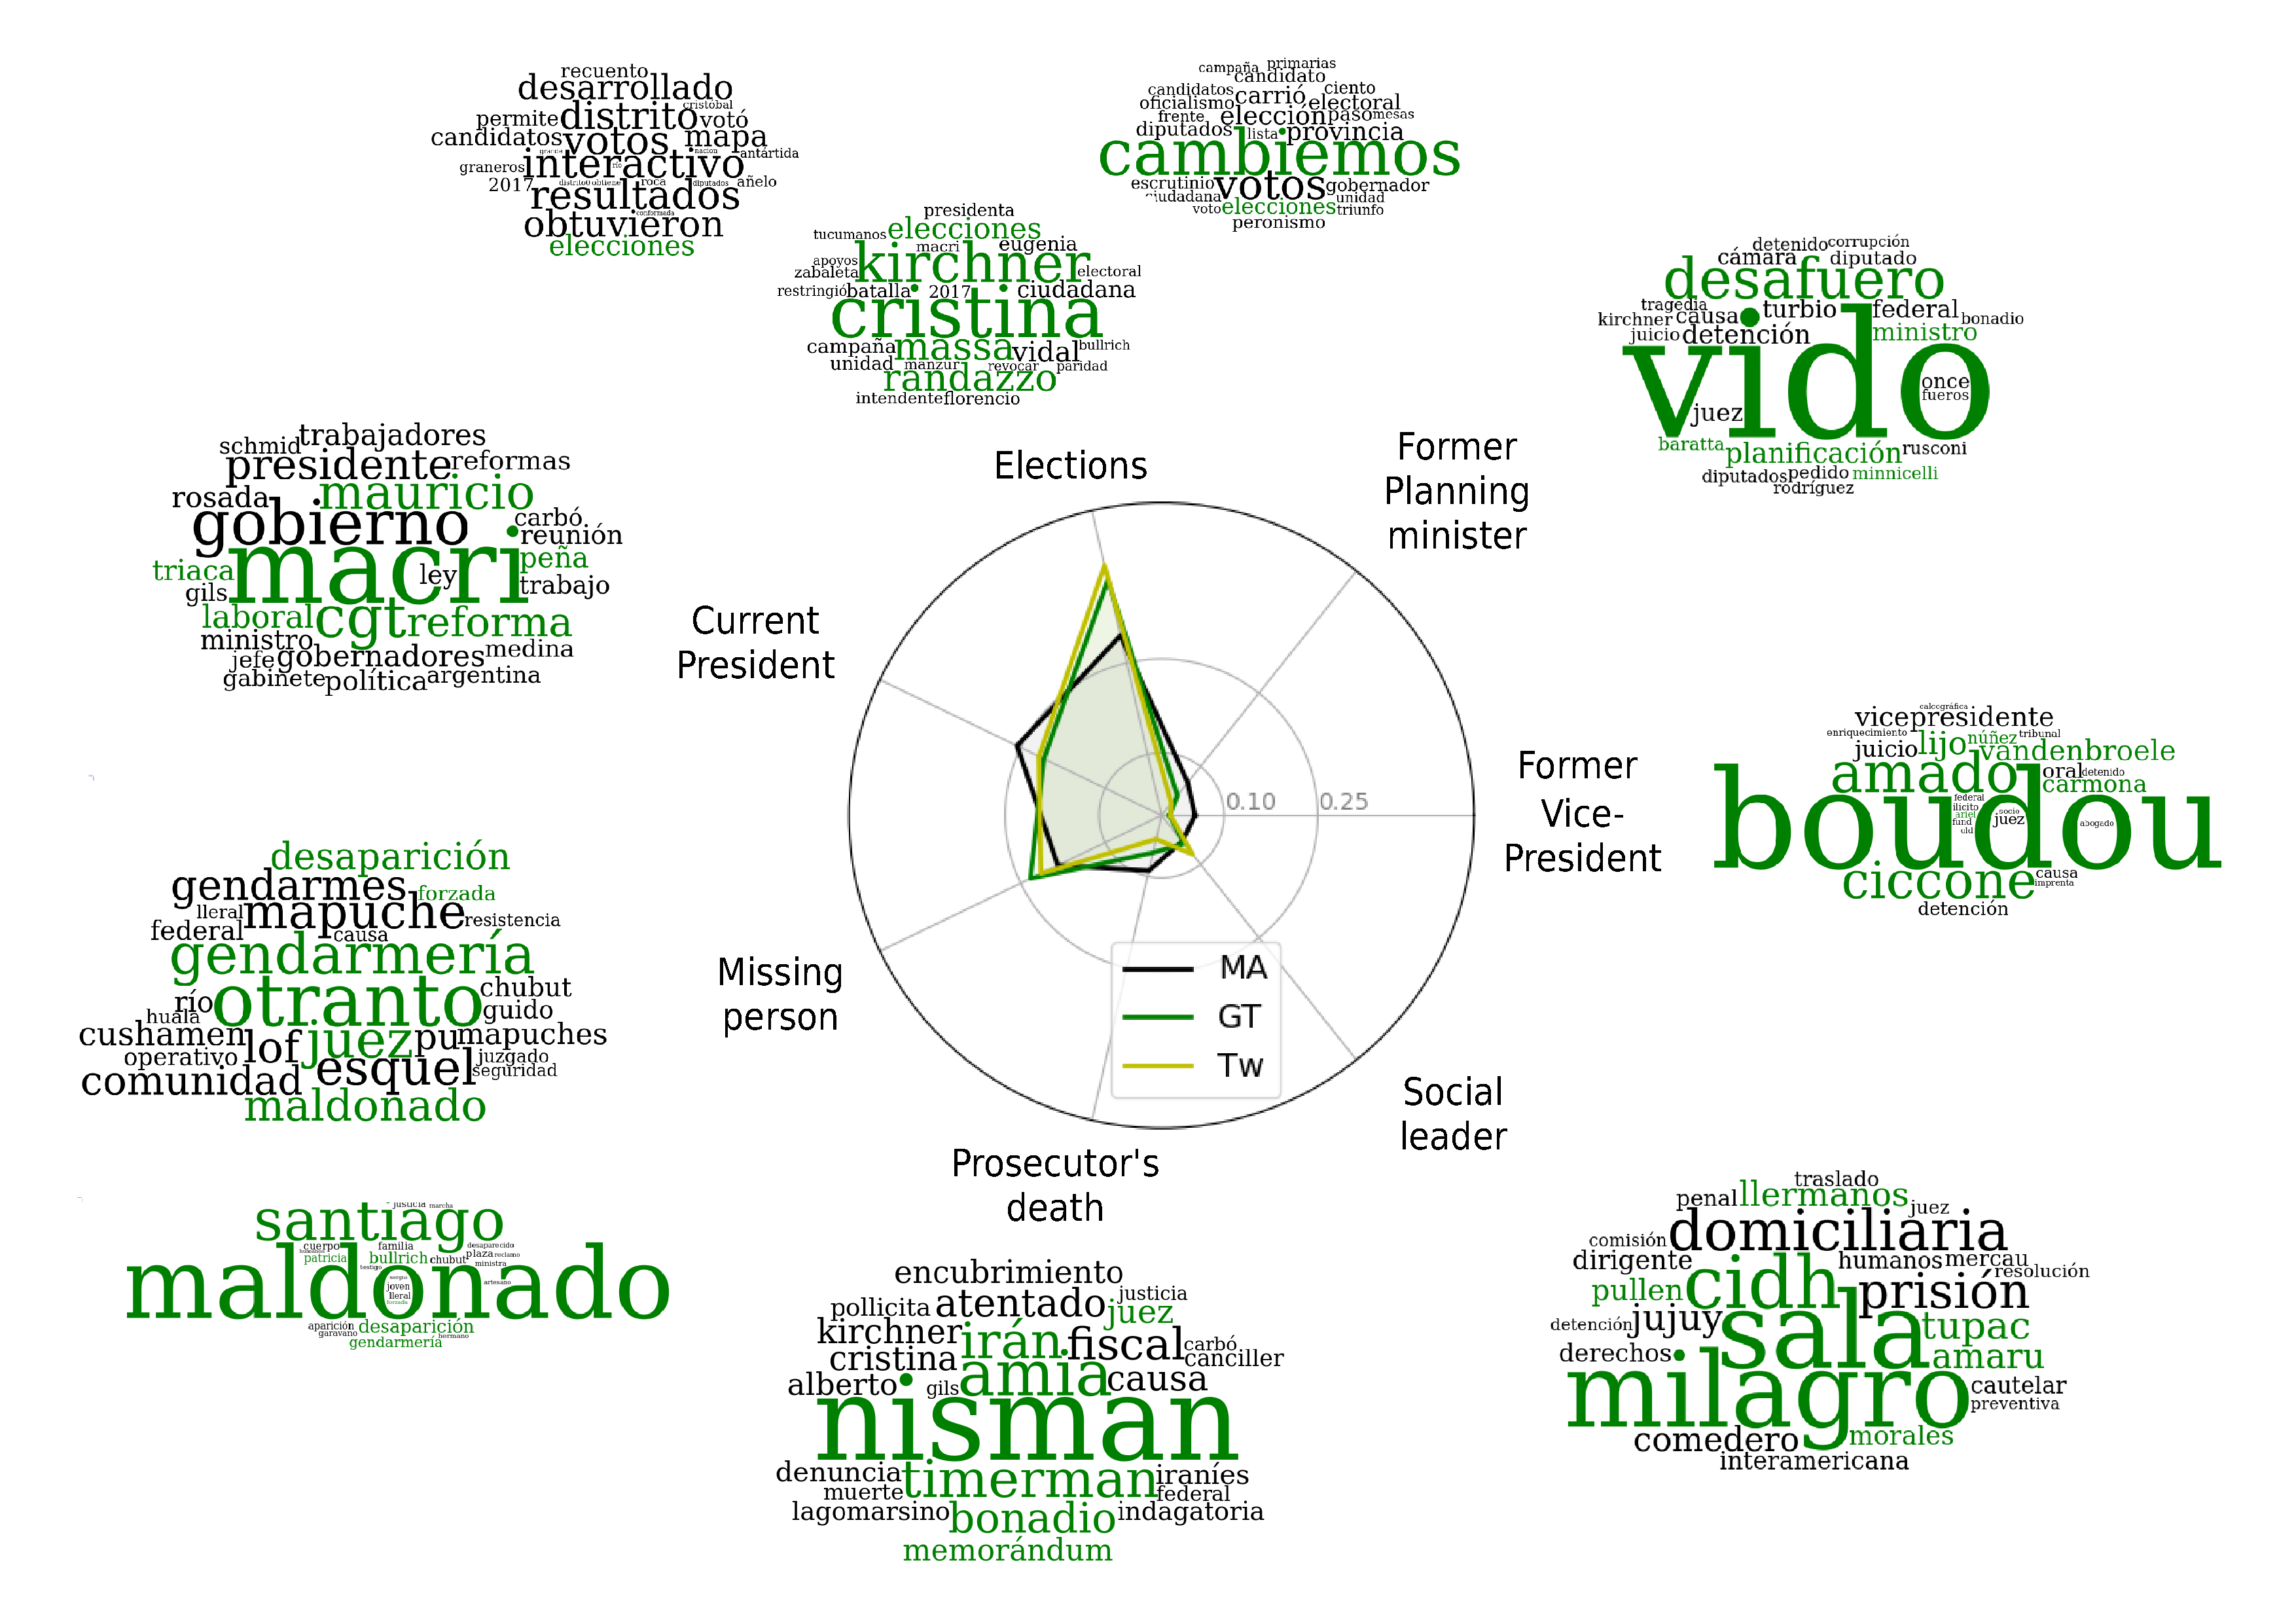
\includegraphics[width = \textwidth]{images/Fig1.pdf}
\caption{\textbf{Radar plots of the Media and Public Agendas represented by the ten topic distribution and their corresponding wordclouds.} The Public Agenda is represented either by Google Trends (GT) and Twitter (Tw). 
Topics names are introduced together with the wordclouds containing the most important keywords involved in the definition of each topic. In green color we show the keywords used to define the topics in the Google Trends and Twitter queries (see table \ref{table:gt_all_correlation}) and therefore in our construction of the Public Agenda.}
\label{fig:topics_wordclouds}
\end{figure}


% Global Agenda figure!!!
\begin{figure}[h]
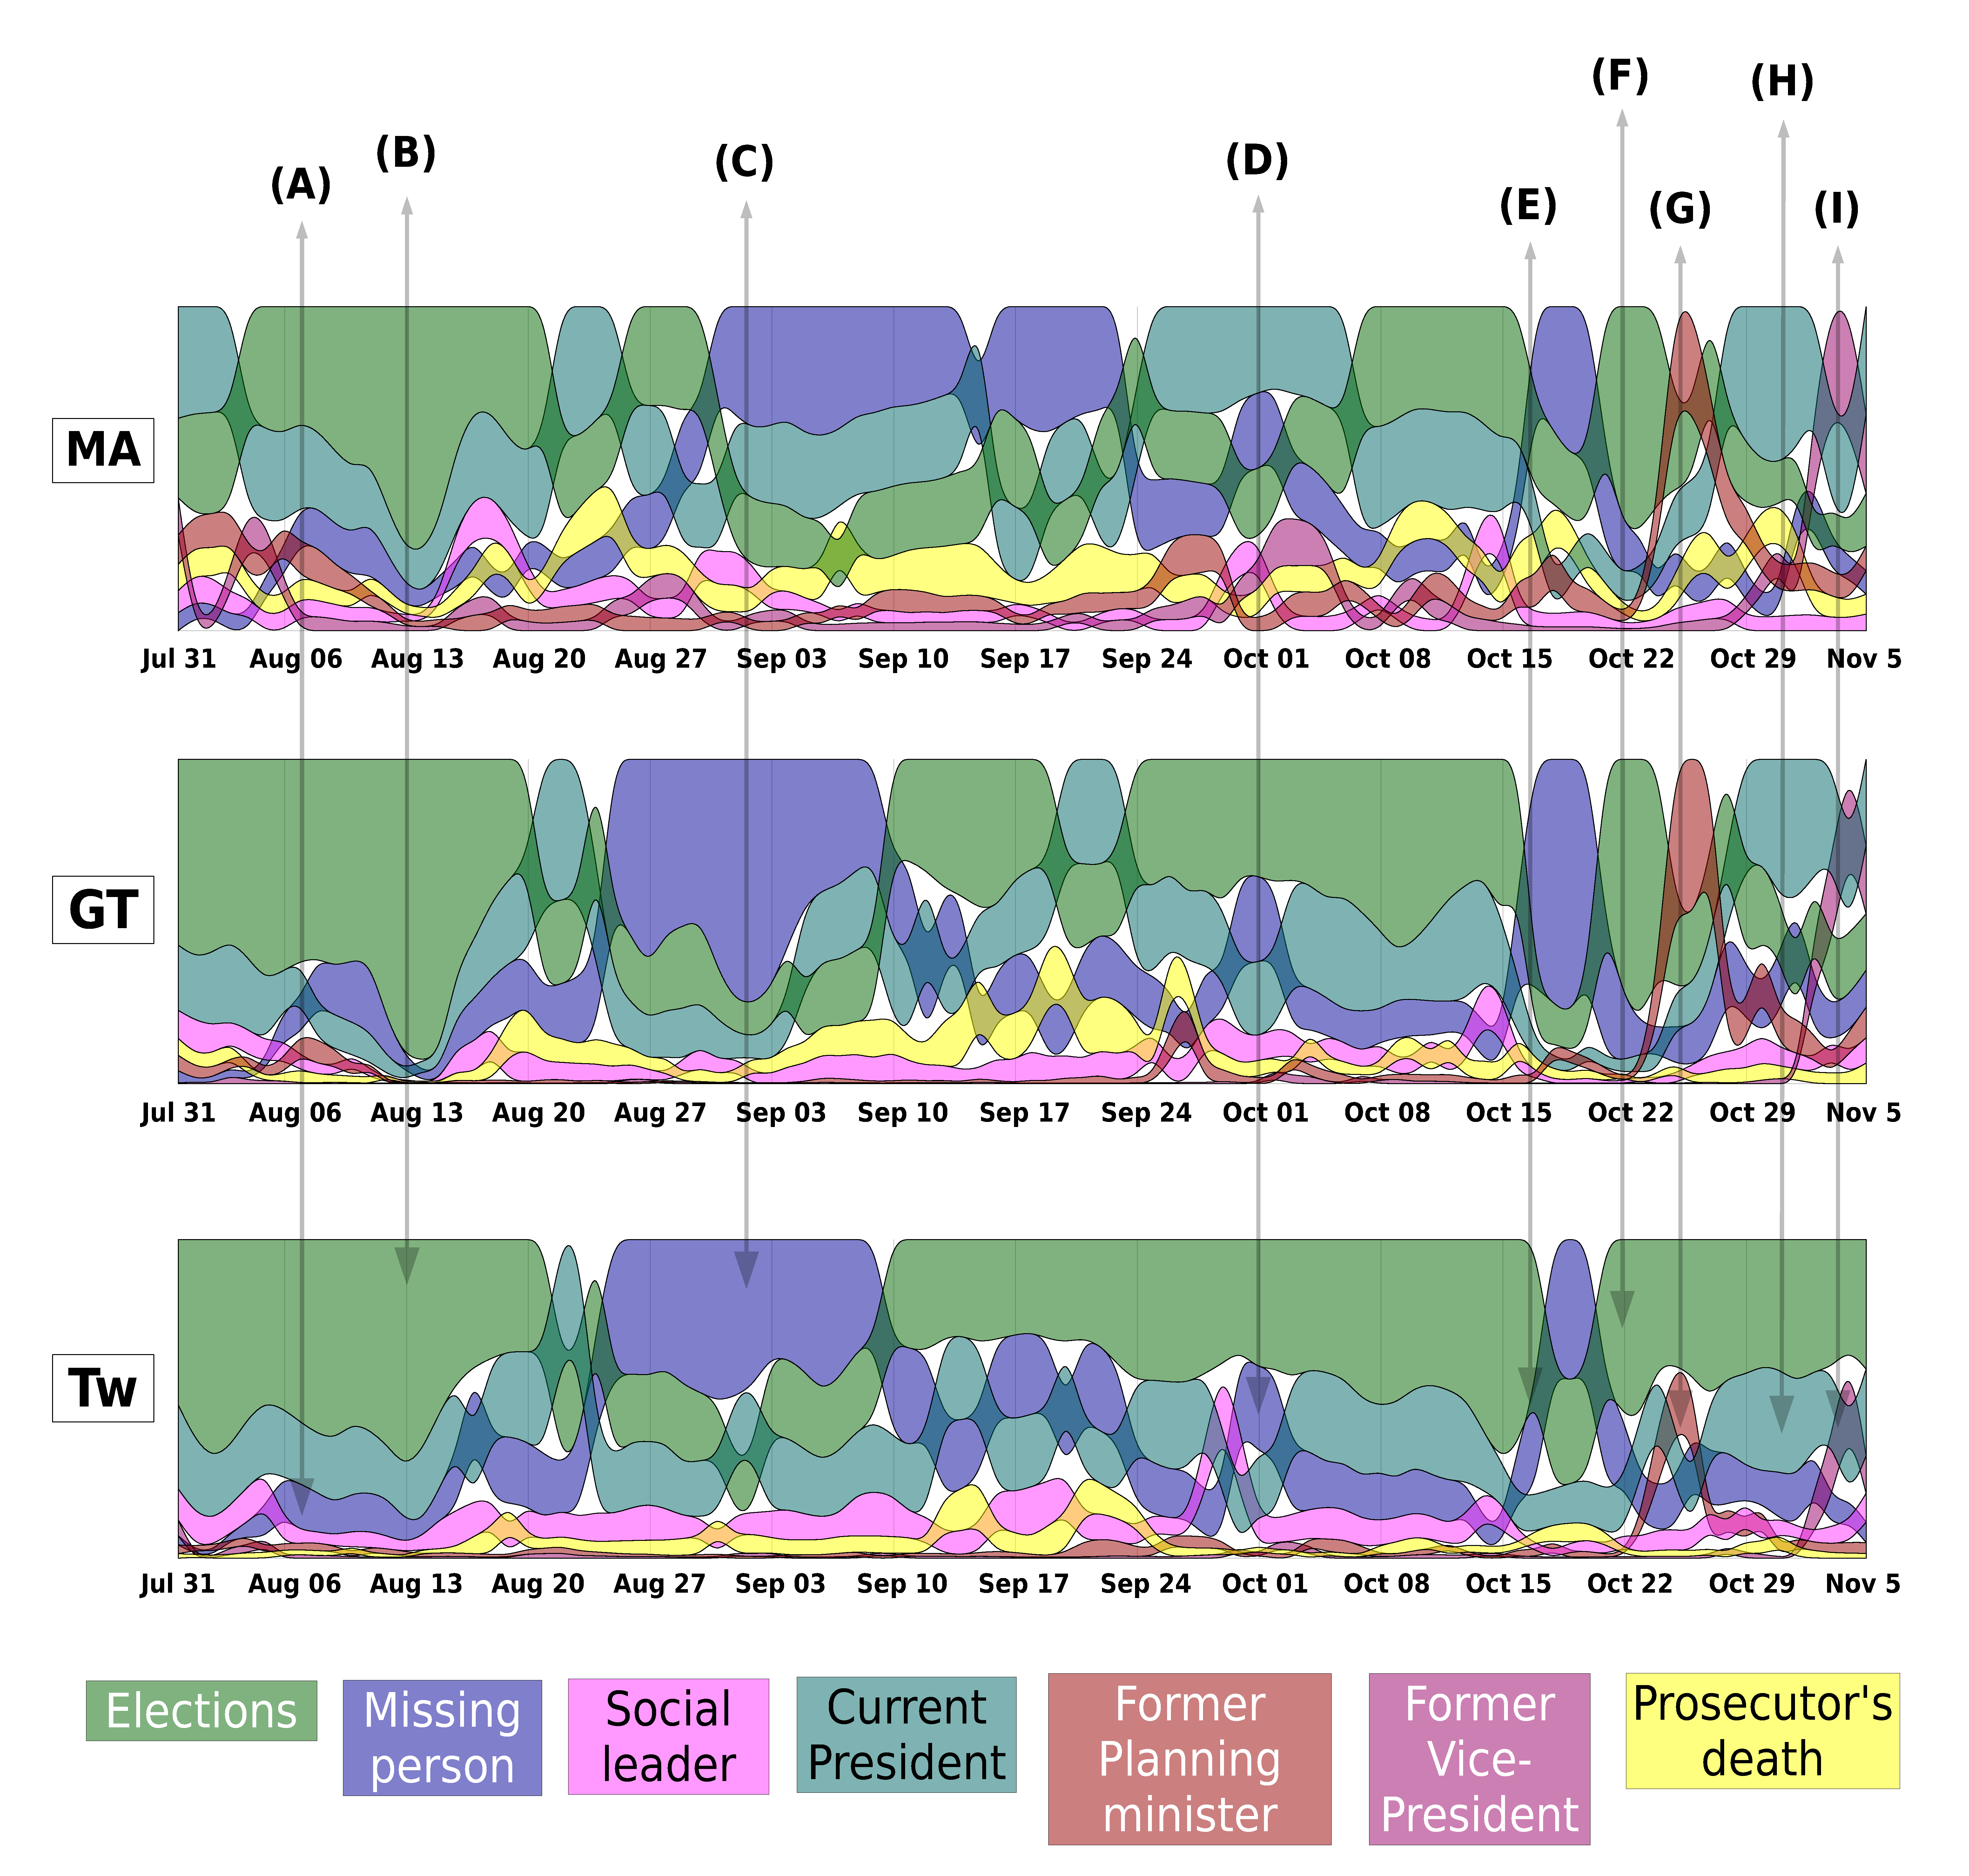
\includegraphics[width = \textwidth]{images/Fig2.pdf}
\caption{\textbf{Bump graph of the Media Agenda (MA) and Public Agenda extracted from Google Trends (GT) and Twitter (Tw)}. The curves width and their ordering are related to the topics relative weight. Some important events related to the topics are pointed out:
\textbf{A}: First news about Santiago Maldonado's disappearance;
\textbf{B}: Primary elections;
\textbf{C}: March one month after Santiago Maldonado's disappearance;
\textbf{D}: March two months after Santiago Maldonado's disappearance;
\textbf{E}: Appearance of Santiago Maldonado's body;
\textbf{F}: General elections;
\textbf{G}: Julio De Vido's detention;
\textbf{H}: Debates on labor reform;
\textbf{I}: Amado Boudou's detention.
A more detailed explanation is given in section \ref{sec:Context}.}
\label{fig:all_agenda}
\end{figure}


% Table with queries and correlations
%\begin{table}[h]
\centering
\resizebox{\textwidth}{!}{\begin{tabular}{llccc}
\toprule
& Google Trends query & Correlation MA and Gt & MA and Twitter & Gt and Twitter \\ 
\midrule
Elections & elecciones + cambiemos + cristina kirchner + massa + randazzo & \textbf{0.81} & \textbf{0.59} & \textbf{0.75} \\
Missing person & santiago maldonado + juez otranto + patricia bullrich + gendarmería + desaparición forzada & \textbf{0.68} & \textbf{0.76} & \textbf{0.89} \\
Former Planning minister & de vido + desafuero + ministro de planificación + minnicelli + baratta & \textbf{0.92} & \textbf{0.82} & \textbf{0.87} \\
Current President & mauricio macri + cgt + reforma laboral + peña + triaca & \textbf{0.77} & \textbf{0.75} & \textbf{0.63} \\
Social leader & milagro sala + cidh + tupac amaru + pullen llermanos + morales & \textbf{0.49} & \textbf{0.25(*)} & \textbf{0.57} \\
Prosecutor's death & nisman + amia + memorándum con irán + timerman + juez bonadio & \textbf{0.56} & \textbf{0.59} & \textbf{0.75} \\
Former Vice-President & amado boudou + ciccone + ariel lijo + vandenbroele + núñez carmona & \textbf{0.90} & \textbf{0.92} & \textbf{0.97}\\
\bottomrule
\end{tabular}}


\caption{Queries performed in Google Trends in order to made up the Public Agenda. 
We also shown the correlation between the topics' temporal profiles of the Public Agenda and their counterpart in Media Agenda.
All correlation values are statistical significant ($p < 10^{-9}$), except (*) which is significant with $p < 0.05$.}
\label{table:gt_all_correlation}
\end{table}


\begin{table}[h]
\centering
\resizebox{\textwidth}{!}{\begin{tabular}{lp{10cm}}
\toprule
Topic's name & Google Trends query \\ 
\midrule
Elections & elecciones + cambiemos + cristina kirchner + massa + randazzo \\
Missing person & santiago maldonado + juez otranto + patricia bullrich + gendarmería + desaparición forzada \\
Former Planning minister & de vido + desafuero + ministro de planificación + minnicelli + baratta \\
Current President & mauricio macri + cgt + reforma laboral + peña + triaca \\
Social leader & milagro sala + cidh + tupac amaru + pullen llermanos + morales \\
Prosecutor's death & nisman + amia + memorándum con irán + timerman + juez bonadio \\
Former Vice-President & amado boudou + ciccone + ariel lijo + vandenbroele + núñez carmona \\
\bottomrule
\end{tabular}}
\caption{Queries used in Google Trends in order to build the Public Agenda.}
\label{table:gt_queries}
\end{table}

\begin{table}[h]
\centering
\resizebox{\textwidth}{!}{\begin{tabular}{lccc}
\toprule
Topic's name & Correlation MA and GT & MA and Twitter & GT and Twitter \\ 
\midrule
Elections & \textbf{0.81} & \textbf{0.59} & \textbf{0.75} \\
Missing person & \textbf{0.68} & \textbf{0.76} & \textbf{0.89} \\
Former Planning minister & \textbf{0.92} & \textbf{0.82} & \textbf{0.87} \\
Current President & \textbf{0.77} & \textbf{0.75} & \textbf{0.63} \\
Social leader & \textbf{0.49} & \textbf{0.25(*)} & \textbf{0.57} \\
Prosecutor's death & \textbf{0.56} & \textbf{0.59} & \textbf{0.75} \\
Former Vice-President & \textbf{0.90} & \textbf{0.92} & \textbf{0.97}\\
\bottomrule
\end{tabular}}
\caption{Correlation between the topics' temporal profiles of the Public Agenda and their counterpart in Media Agenda.
All correlation values are statistical significant ($p < 10^{-9}$), except (*) which is significant with $p < 0.05$.}
\label{table:gt_all_correlation}
\end{table}


\par The figures introduced above show not only the topics and their differences between Agendas, but also the dynamics of the topics.  For instance, we can see in the radar plot of figure \ref{fig:topics_wordclouds}, a greater interest of the audience in the topic \emph{Missing person} than the Media, or inversely in the topic \emph{Prosecutor's death}, at least in the analyzed time-lapse. 
We can also observe a great similarity between \textbf{GT} and \textbf{Tw} agendas which both are different faces of the Public Agenda.

\par On the other hand, figure \ref{fig:all_agenda} allow us to appreciate how the main topic change in time and have a glance of the qualitative differences between agendas.
The linear correlations shown in table \ref{table:gt_all_correlation} are  positive and statistically significant in all the cases, This can be interpreted as a validation of the topics found in the corpus and the keywords that describe it. 
Even though it is expected that the Media's and public's interest should generally follow a similar a pattern due to the external events, we are interested in those periods where they significantly differ. 
A non positive (or a non significant) correlation may imply, besides the obvious conclusion of agenda's disengagement, that we could eventually fail in properly detect the keywords or features that describe a particular topic, so the Google Trends' or Twitter's pattern would not be able to reflect a similar behavior that its counterpart in the Media.

\subsection{A quantitative description of the Agendas}

\subsubsection{Agenda diversity}

% Agenda diversity

\par In order to quantify the diversity of the Agendas, we start by representing them as distributions in the topic's space. 
Following \cite{boydstun2014importance}, we calculate the normalized Shannon's entropy ($H$, see eq.\ref{eq:shannon_entropy}) in order to measure the diversity of the \textbf{MA} and \textbf{PA}.
\par In figure \ref{fig:shannon_entropy_agendas} we can see the value of $H$ as a function of time, where it can be focused in those periods of time where the diversity is lower than usual. This effect is notoriously more pronounced in the Public Agenda giving by \textbf{GT}, and in particular in four specific days  where can be detected four local minima of Shannon's entropies. Three of them are outliers as defined in section \ref{sec:MatMeth}, two of them from \textbf{GT} and one from \textbf{Tw}. 

\par A lower value in the agenda's diversity is due to the fact that the most important topic attracts practically all the attention of the public and the media.
In the radar plots included in figure \ref{fig:shannon_entropy_agendas} we can see that two of these outliers (\textbf{a} and \textbf{d}) belong to the topic \emph{Elections} and coincide with the primary and general legislative elections that took place in August 13th and October 22th. 
In all the agendas these points where detected as outliers except point (d) in Twitter Agenda. Why is that? The radar plot of the Twitter agenda for this day displays an association between the topic \emph{Elections} and the \emph{Current President} which could be decreasing the important this topic.
Discussions in Twitter about elections appear also in point (c), when the other agendas seems to be more diverse. 
On the other hand, we focused in point (b), despite not being detected as a outlier, because it belong to the topic \emph{Missing person} and this date correspond to the rally that took place one month after the disappearance of Santiago Maldonado (see section \ref{sec:Context}). It is important to notice that, the Shannon's Entropy of GT Agenda displays a minimum (collapsing agenda) not shown neither in the Media nor in the Twitter Agendas.
We emphasize the discussion about this topic because we can appreciate  interesting facts that appear along the analysis.

\begin{figure}[h]
\centering
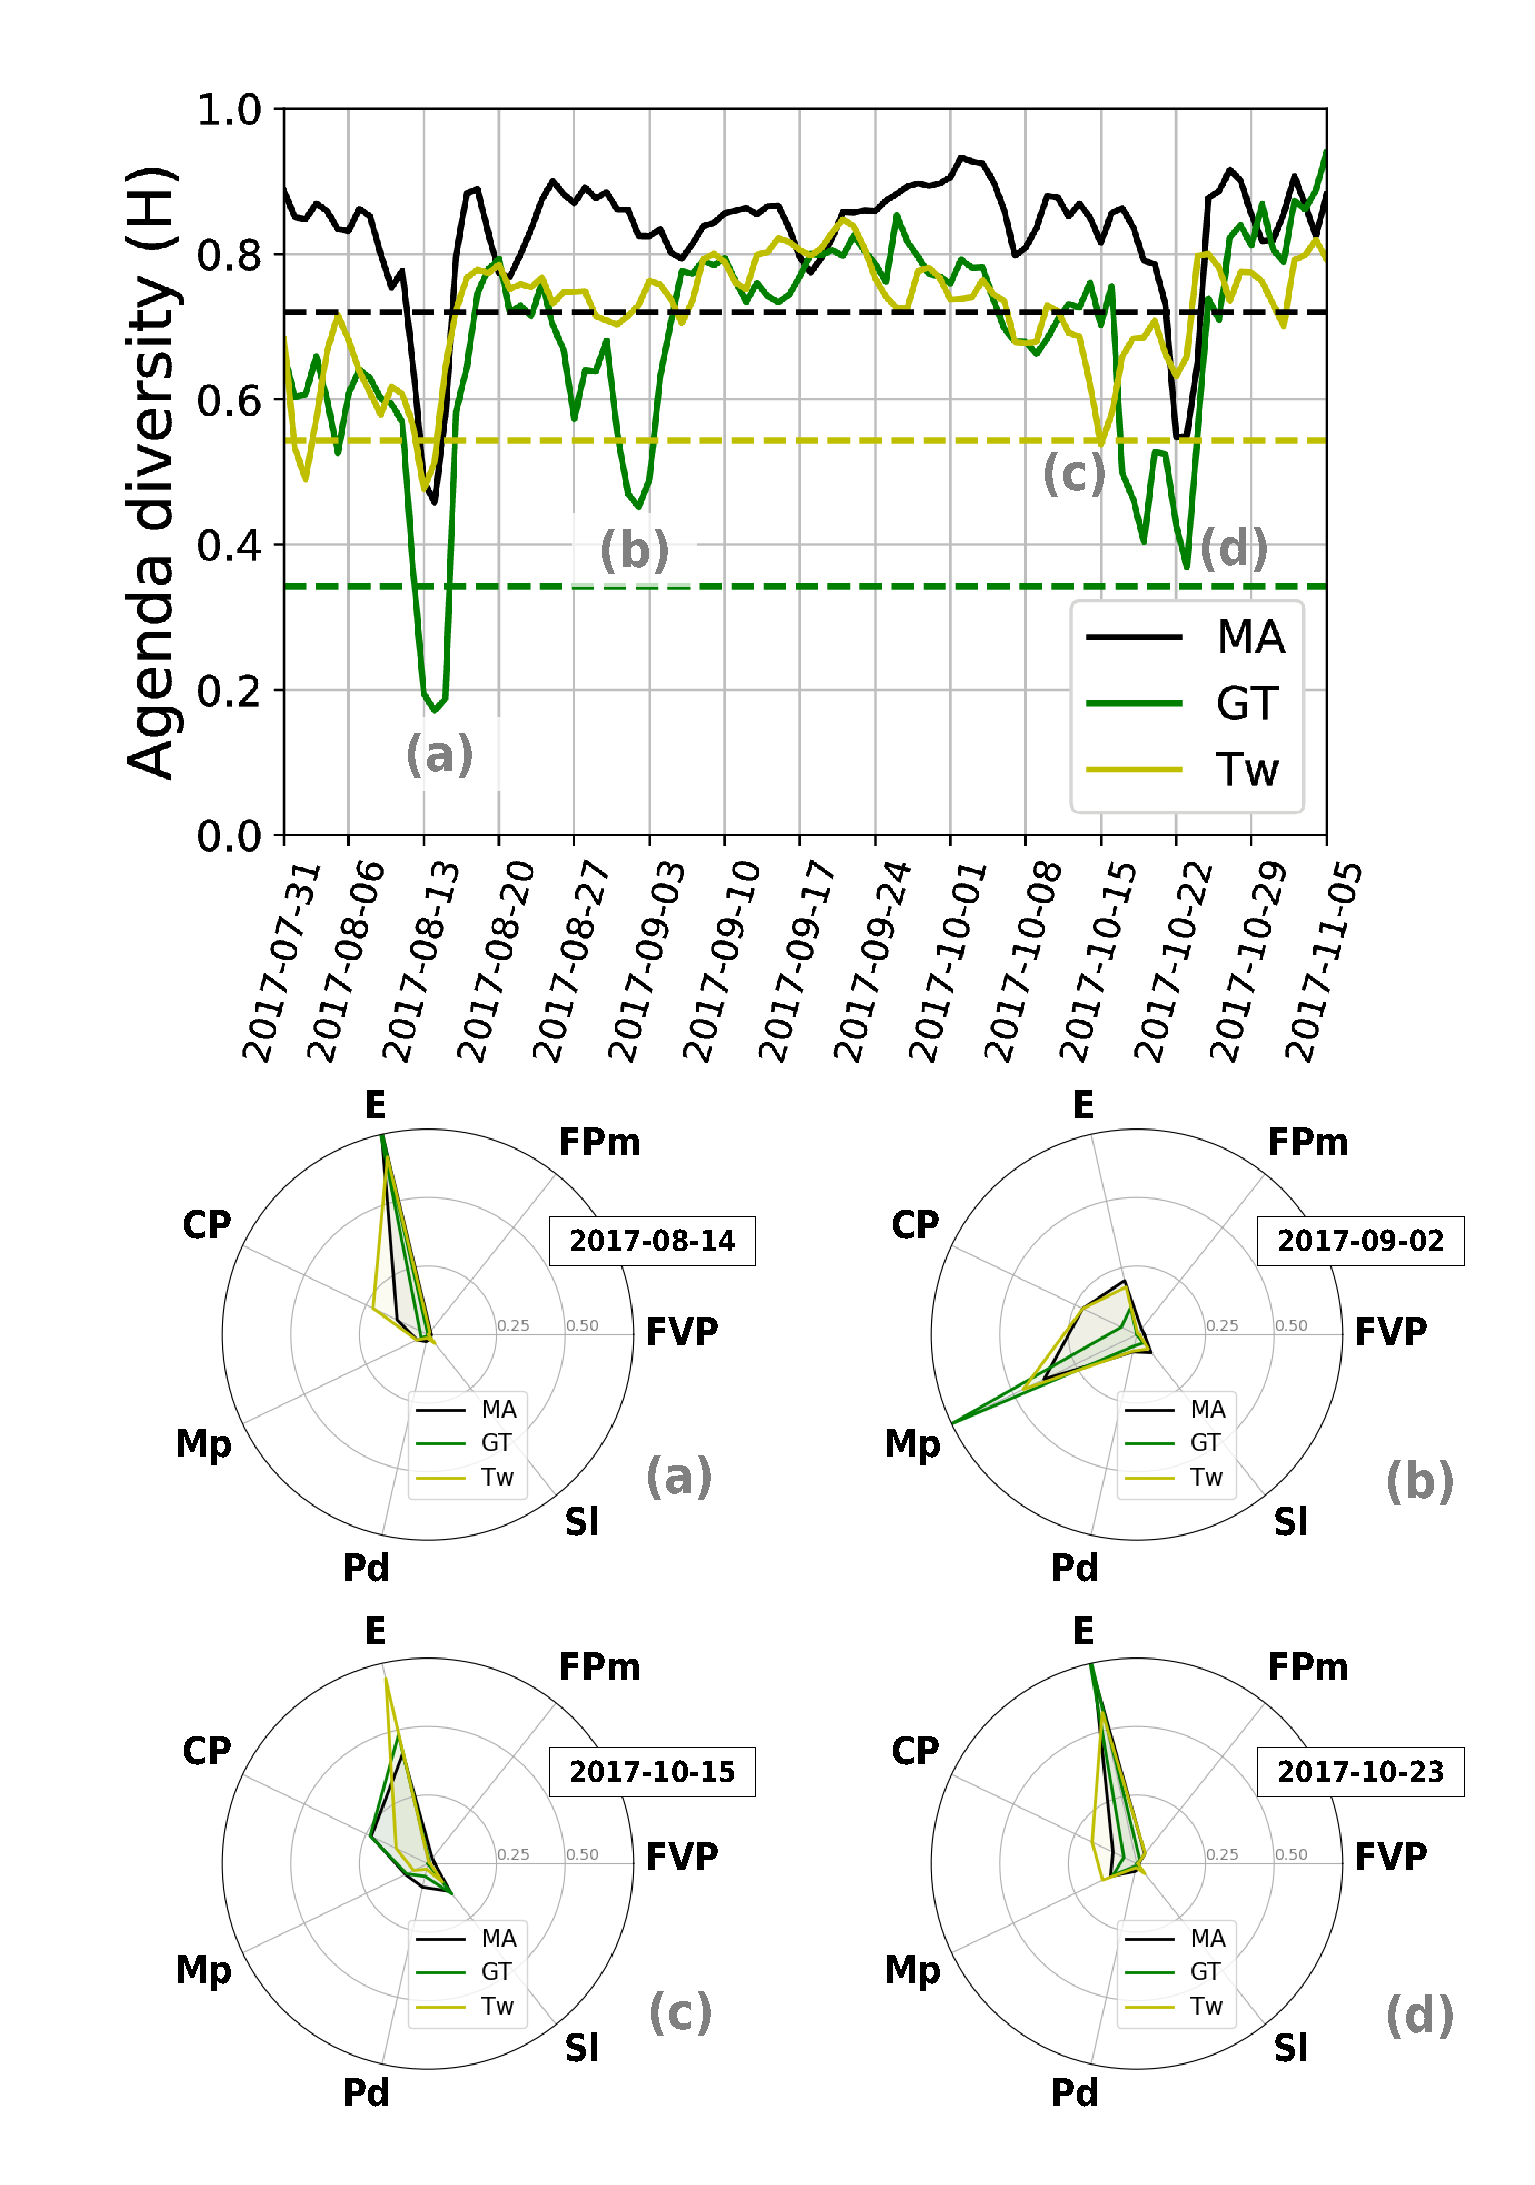
\includegraphics[height=0.75\textheight]{images/Fig3.pdf}
\caption{\textbf{Shannon entropy (H) as a measure of agenda diversity.} The Public Agenda show a less diverse behavior than the Media Agenda as can be seen in the left figure. The horizontal lines are the lower inner fences of each signal in order to identify outliers. The related radar plots shows that those dates when the agenda has a low diversity, the most important topic catches the most public’s attention. \textbf{E}: Elections; \textbf{FPm}: Former Planning minister; \textbf{FVP}: Former Vice-President; \textbf{Sl}: Social leader; \textbf{Pd}: Prosecutor's death; \textbf{Mp}: Missing person; \textbf{CP}: Current President.}
\label{fig:shannon_entropy_agendas}
\end{figure}

\par From the measure of $H$ we can also see that the median of the Public Agenda diversity is statistical significant lower than the Media Agenda's one.
Specifically $H_{Gt} = 0.73$ and $H_{Tw} = 0.74$ are statistical significant lower than $H_{MA} = 0.85$ with $p < 10^{-18}$, while there is no significant difference between the first two. 
However from figure \ref{fig:shannon_entropy_agendas} we can see that \textbf{GT} shows more abrupt dropouts in the diversity in response to specific events.
We conclude that its an important fact about audience behavior: given a finite set of topics, \textbf{the Public Agenda is less diverse than the Media Agenda}, because the public seems to focus more in the most important topic than the Media can do, maybe due to editorial decisions.

\subsubsection{Distance between Media and Public Agenda's }

% Jensen-Shannon distance between PA and MA

\par Given our interpretation of  the Agendas and time-evolving distributions, we can  compare them by computing the Jensen-Shannon distance. In this context, outliers in selected dates will correspond to divergences between Public and Media Agenda, i.e., specific events where the public interest do not match with media offer.
In figure \ref{fig:jensen_shannon_gt} we show the Jensen-Shannon distance between Media and Publics Agendas as a function of time. We focus in three points that seems to be relevant enough. In all cases, the topic distributions at that particular dates displayed by  the radar plots shows that a greater distance is associated with a more interest of public in the topic \emph{Missing person}. 
\par Points \textbf{(c)} and \textbf{(d)} shows that both the Public and the Media highlight this topic, but the Media do not disregard other topics, so the corresponding distance between them can be interpreted  of another way of see  the diversity effect discussed in the last section.

\par On the other hand,  points \textbf{(a)} (we take this point due to be a local maximum despite not being an outlier) and \textbf{(b)} seem to show an interest of the public in the topic \emph{Missing person} which it is not reflected in the Media.  In figure \ref{fig:all_agenda} we can see that this topic becomes the most important in public's interest (both \textbf{GT} and \textbf{Tw}) days before that  it happen in the Media Agenda. It can be associates  with a social networks (like Facebook and Twitter) campaign  in favor  of the appearance of Santiago Maldonado ("The missing person") that took place on  August 26th. It was very important and and was initially underestimated by the main Media outlets in Argentina (see section \ref{sec:Context}). 

\par It is important to notice that it is our interpretation of the data based on the knowledge of the context, and  we are not measuring causality between Agendas (we will say a few words about it in section \ref{sec:who_sets}), i.e. we can't say, for instance, that in this case the Public Agenda set the Media Agenda. 
However, the Jensen-Shannon distance, in conjunction with the measurement of the agenda diversity given by the Shannon entropy, give an insight of independent behavior of the Public and the Media, and its identification can be a starting point to study the Media reaction to a change in audience's interests.
 
\begin{figure}[h]
\centering
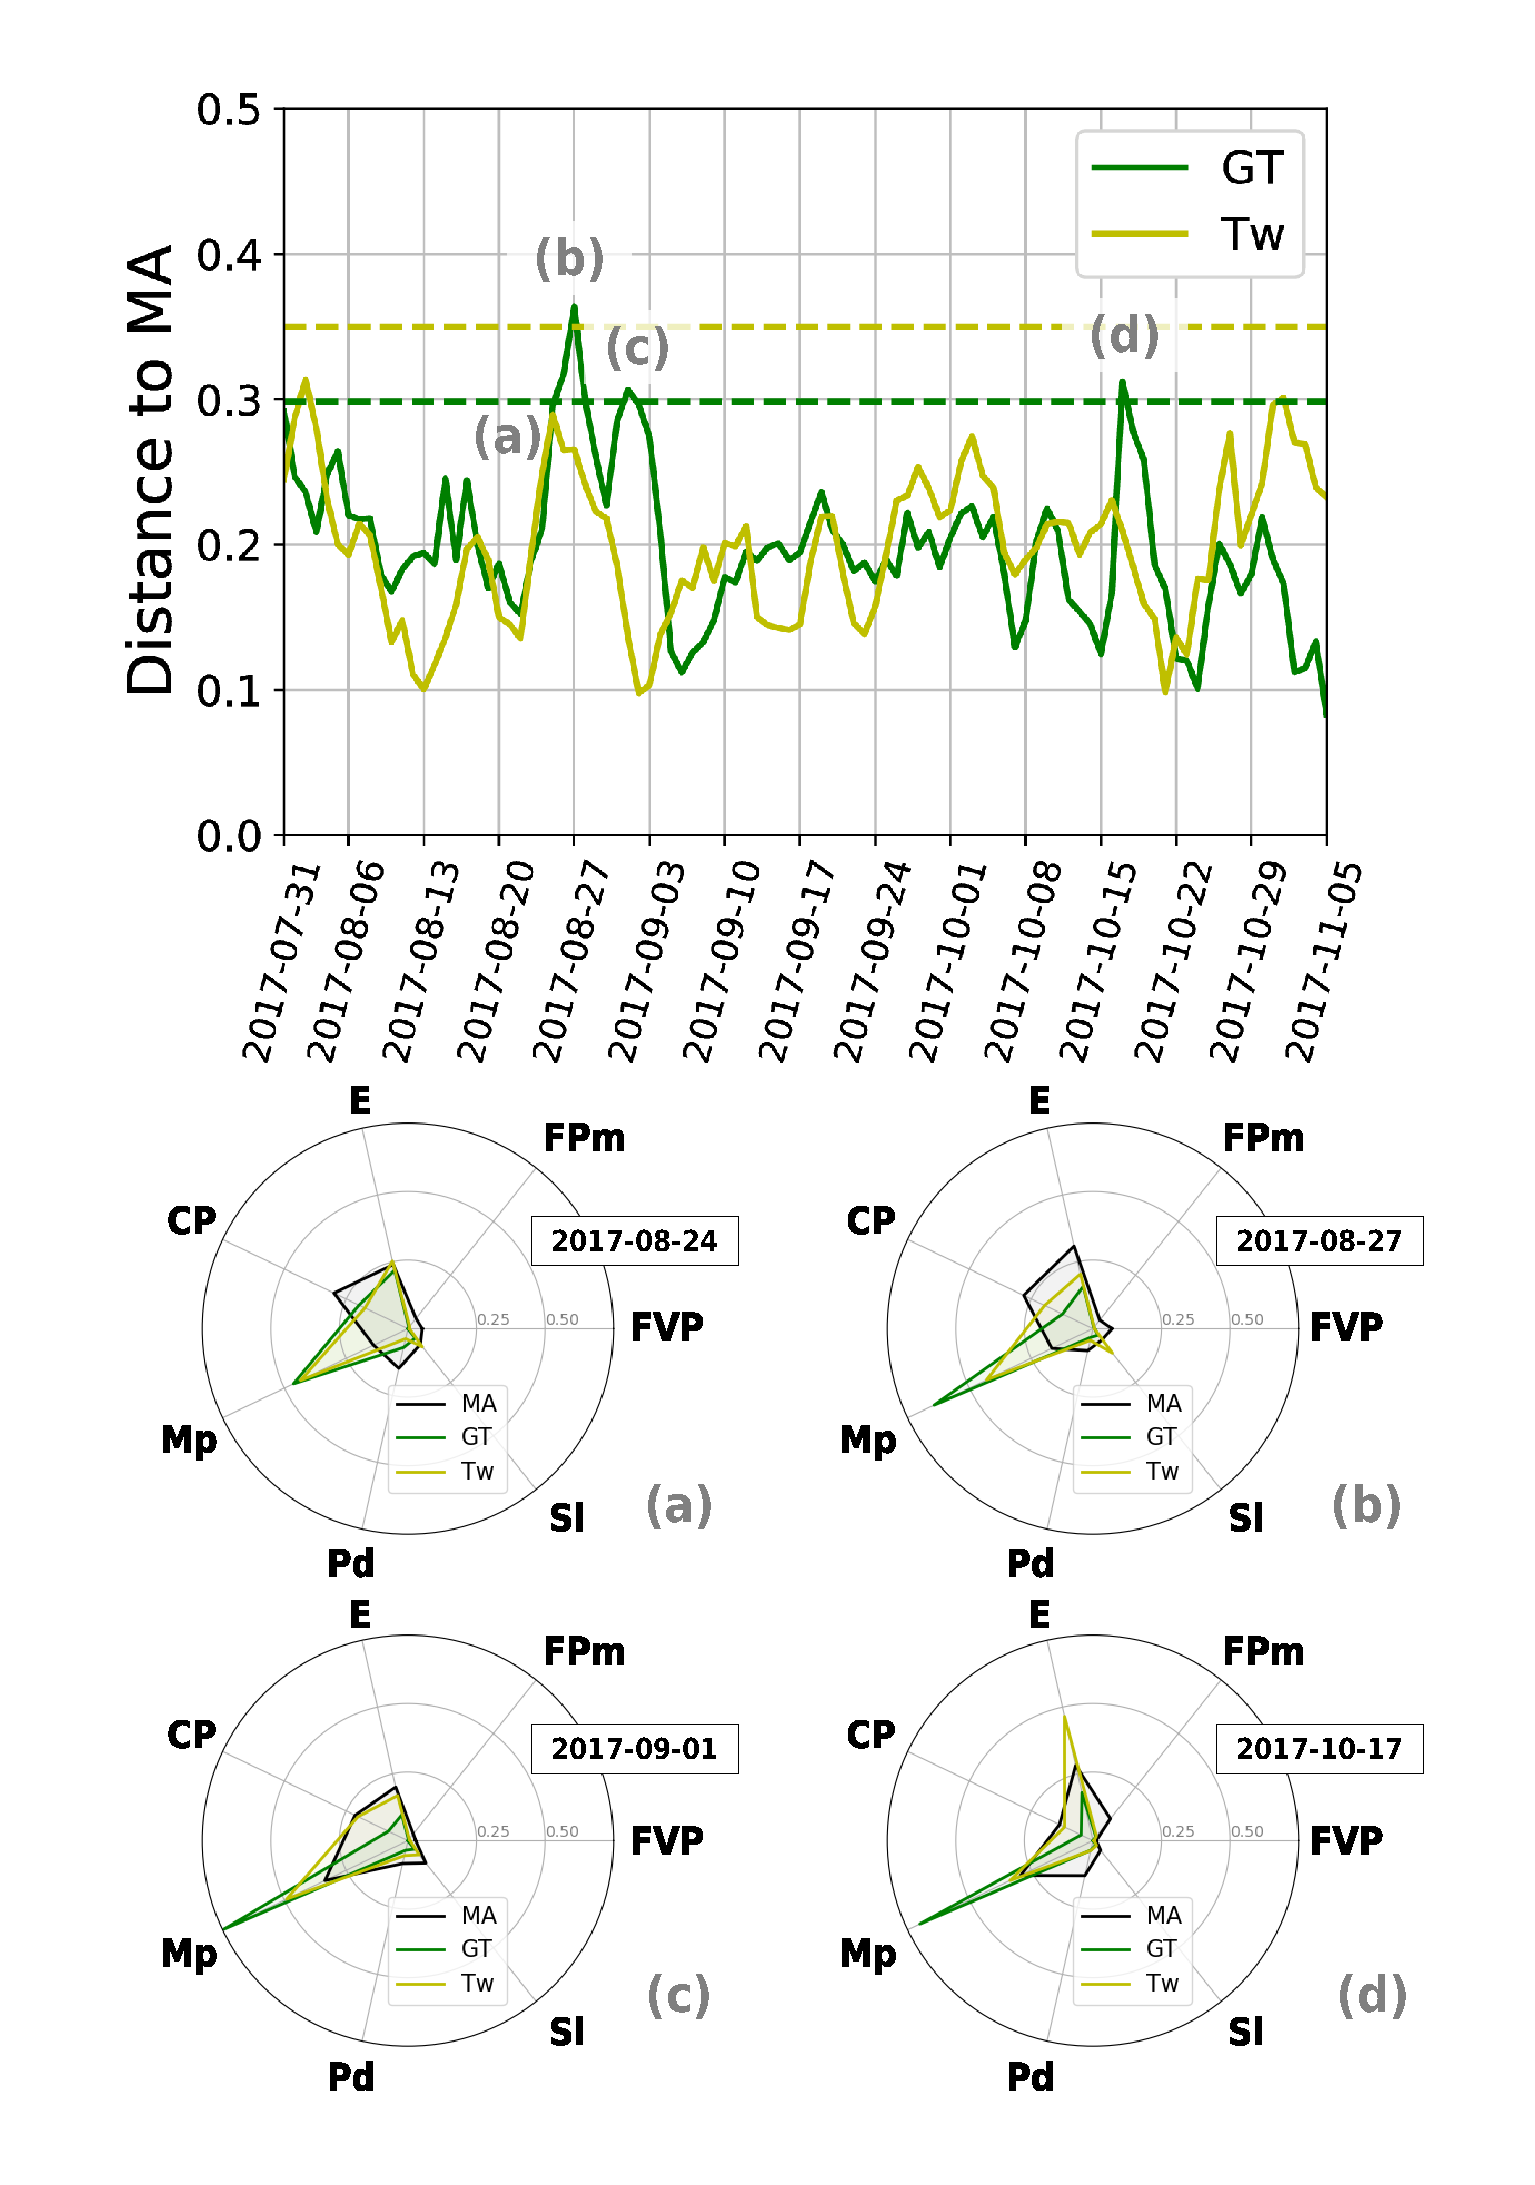
\includegraphics[height = 0.75\textheight]{images/Fig4.pdf}
\caption{\textbf{Jensen Shannon distance between the Media Agenda and the Public Agenda as a function of time} (with upper inner fences pointed out). The larger distances are due to a greater interest of the audience in the topic \emph{Missing person} which leads to lesser interest in the other topics, which the Media has to cover, maybe except in points (a) and (b) where the Media seems not to anticipate the public interest in the mentioned topic. \textbf{E}: Elections; \textbf{FPm}: Former Planning minister; \textbf{FVP}: Former Vice-President; \textbf{Sl}: Social leader; \textbf{Pd}: Prosecutor's death; \textbf{Mp}: Missing person; \textbf{CP}: Current President.}
\label{fig:jensen_shannon_gt}
\end{figure}


\subsection{Agenda bias in different Media outlets}

\par In this section we leave aside the Public Agenda as a whole and we study how the Media agenda of each media outlet. 
In figure \ref{fig:news_agenda} we show the bump charts corresponding to each newspaper analogously to figure \ref{fig:all_agenda}.
The topics are the same introduced in the wordclouds of figure \ref{fig:topics_wordclouds}, but when computing the topics' weights,  the articles are discriminated by newspaper. 
We also show the radar plots showing the average distribution, as made in figure \ref{fig:topics_wordclouds}. 
\par In figure \ref{fig:news_agenda} we can see in a qualitative way the slightly differences between the newspapers' agendas.
For instance, we can see how newspaper called \emph{Pagina 12} gave more importance to the topics \emph{Missing person} and \emph{Social leader}, while it reduces to minimum the coverage of the topic  \emph{Former Planning minister} as the others did.

% Jensen shannon distance of Dynamic way
\begin{figure}[h]
\centering
\includegraphics[width = \textwidth]{images/Fig5.pdf}
\caption{\textbf{Bump charts of newspapers' Agenda and radar plot of the average distributions.} The figure shows, in a qualitative way, the bias in the different newspaper's agendas. For instance, the greater interest of \emph{Pagina 12 (P12)} in the \emph{Missing person} topic and its slightly lower coverage in the \emph{Former Planning minister} respect to the other newspapers.}
\label{fig:news_agenda}
\end{figure}

%\subsubsection{Independent behavior}

\par In other to detect outliers behavior of a given newspaper respect to the others, we again calculate the Jensen-Shannon distance between the newspapers agenda and the Media Agenda.
Note that this is the distance between the distributions of figure \ref{fig:news_agenda} and the top panel of figure \ref{fig:all_agenda}.
\par In figure \ref{fig:jensen_shannon_news} we show the Jensen-Shannon distance as a function of time.
We detect three points as outliers, although we discard the point \textbf{(b)} due to the low information of \emph{Infobae} in that period. 
The other two points corresponds to differences between \emph{Pagina 12} and the other newspapers and correspond to differences in the coverage of the topic \emph{Missing person}.

\par The point \textbf{(a)} corresponds  to the first news of the Santiago Maldonado's disappearance  reported by \emph{Pagina 12} before the primary elections, and in point \textbf{(c)} to  the two months rally after the disappearance took place (see section \ref{sec:Context}). Another difference in point \textbf{(c)} corresponds to a greater coverage of \emph{Pagina 12} in the topic \emph{Social leader} where the others media outlets seem to be more interested in the topic \emph{Former Vice-President}.

% Jensen shannon distance of Dynamic way
\begin{figure}[h]
\centering
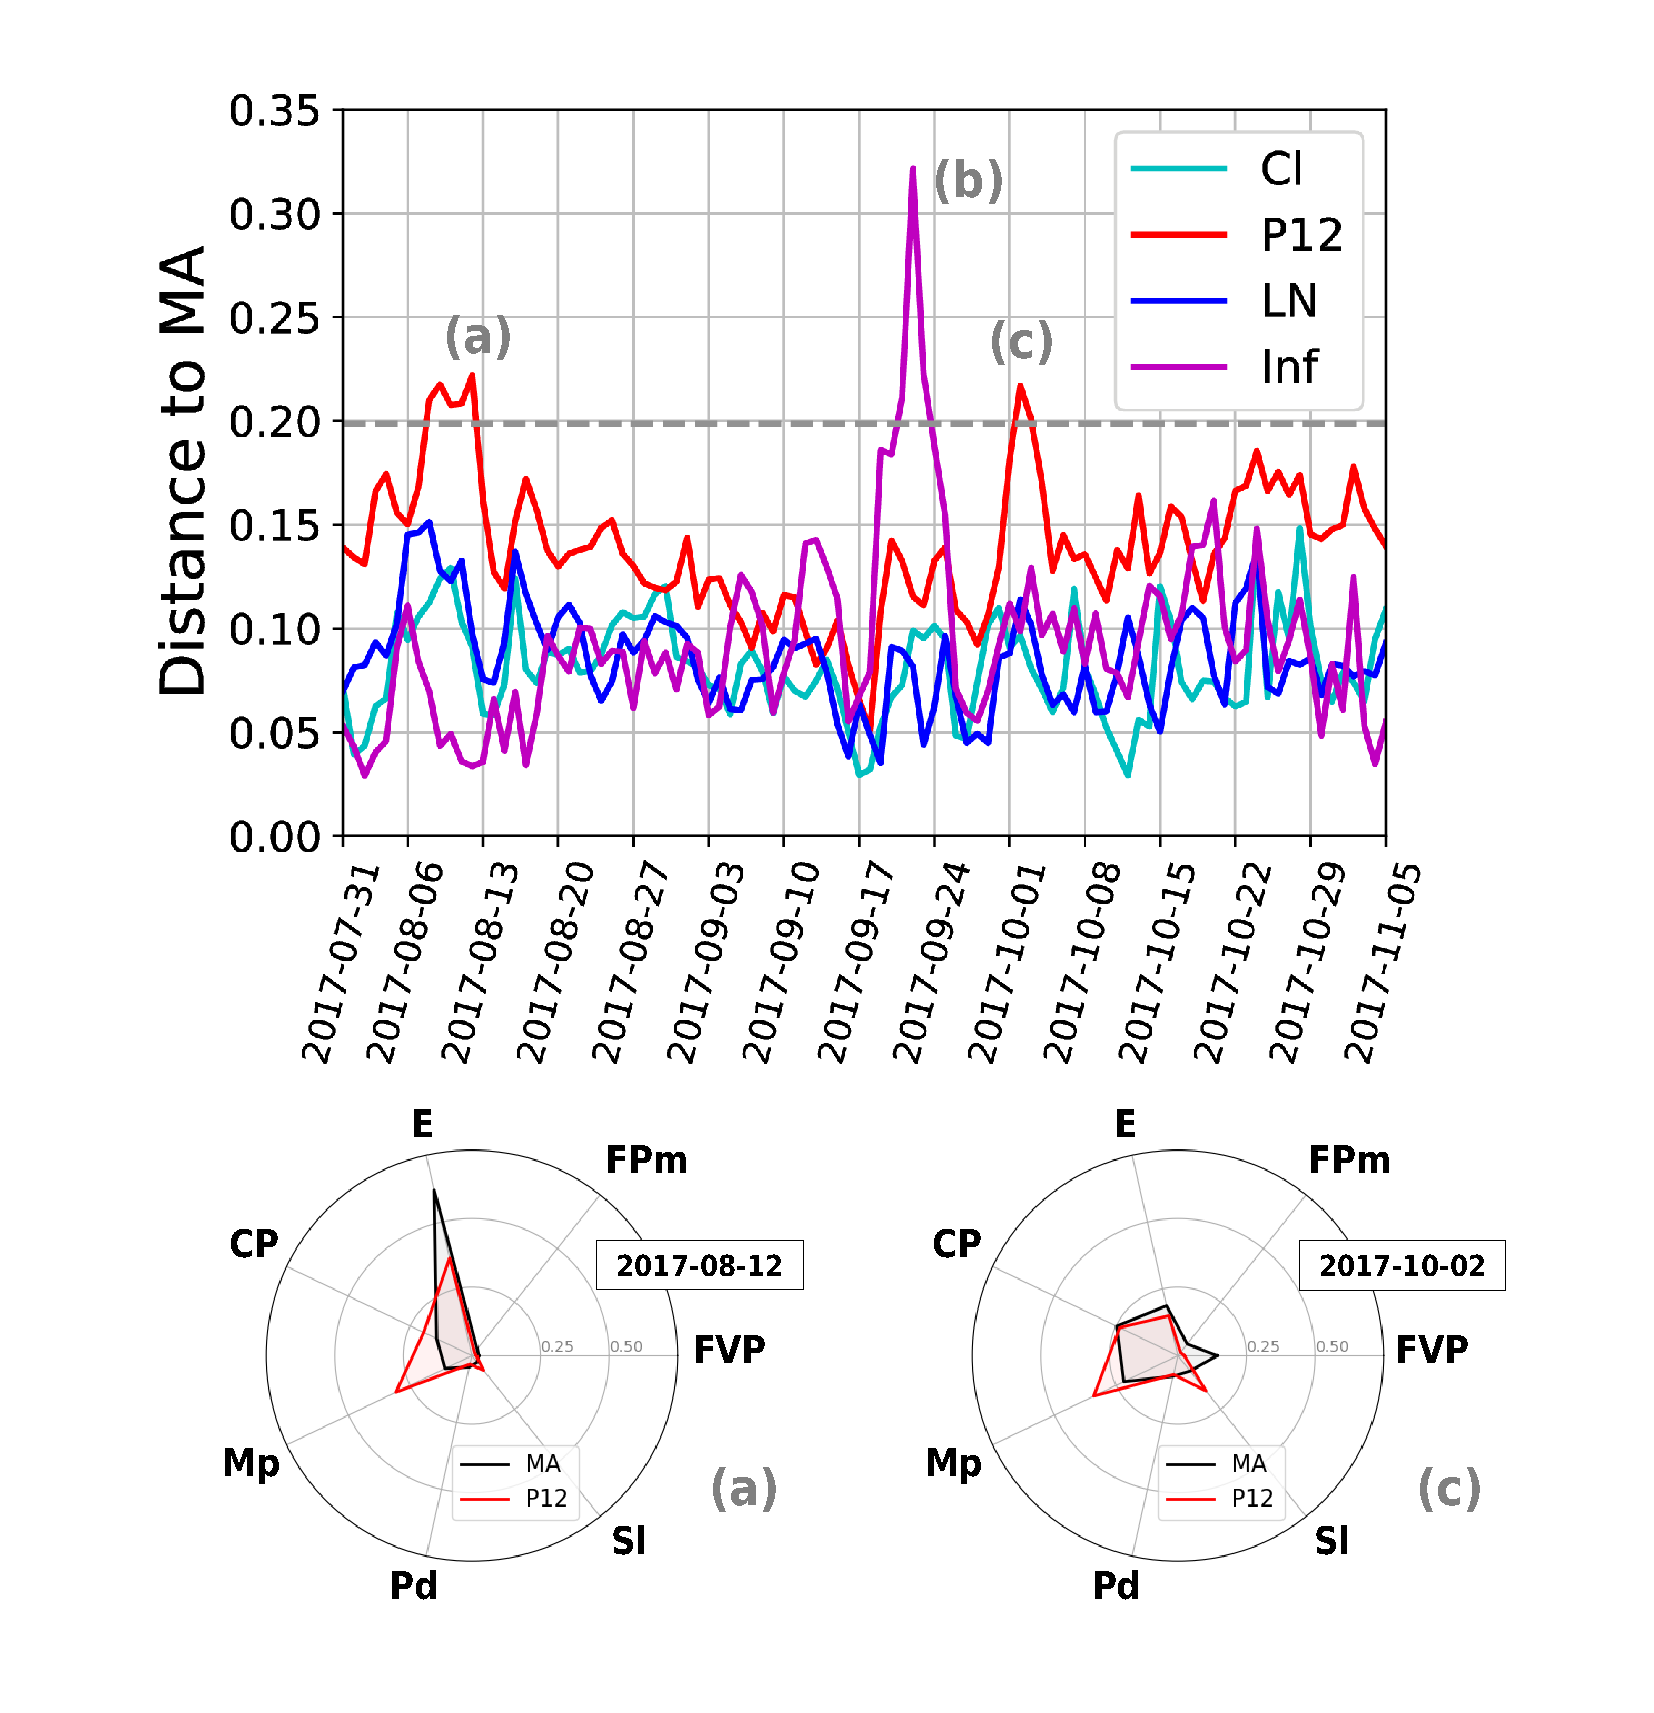
\includegraphics[width = \textwidth]{images/Fig6.pdf}
\caption{\textbf{Jensen-Shannon distance between the newspapers agenda and the Media Agenda as a function of time}. \emph{Pagina 12} shows the more different behavior, motivated again by its interest in the \emph{Missing person} and \emph{Social leader} topics as can be seen in the radar plots which belongs to points (a) and (c). The anomalous behavior of \emph{Infobae} at pint (b) is due to few articles around that date in our database, therefore we ignore its radar plot. \textbf{E}: Elections; \textbf{FPm}: Former Planning minister; \textbf{FVP}: Former Vice-President; \textbf{Sl}: Social leader; \textbf{Pd}: Prosecutor's death; \textbf{Mp}: Missing person; \textbf{CP}: Current President.}
\label{fig:jensen_shannon_news}
\end{figure}


%\subsubsection{Coverage bias}

\par The greater coverage in the topic \emph{Missing person} by \emph{Pagina 12} is even more clear if we inspect the temporal profile of the topic and compare the coverage given by each newspaper. A difference in the coverage is what it is called \emph{coverage bias} [CITA ACA SEBAS].  In figure \ref{fig:topics_temporal_profiles} we show the temporal profile of the topic \emph{Missing person} (panel (a)) and the topic \emph{Former Planning minister} in panel (b), as an example where the behavior is the opposite, as can be seen below.

\begin{figure}[h]
\centering
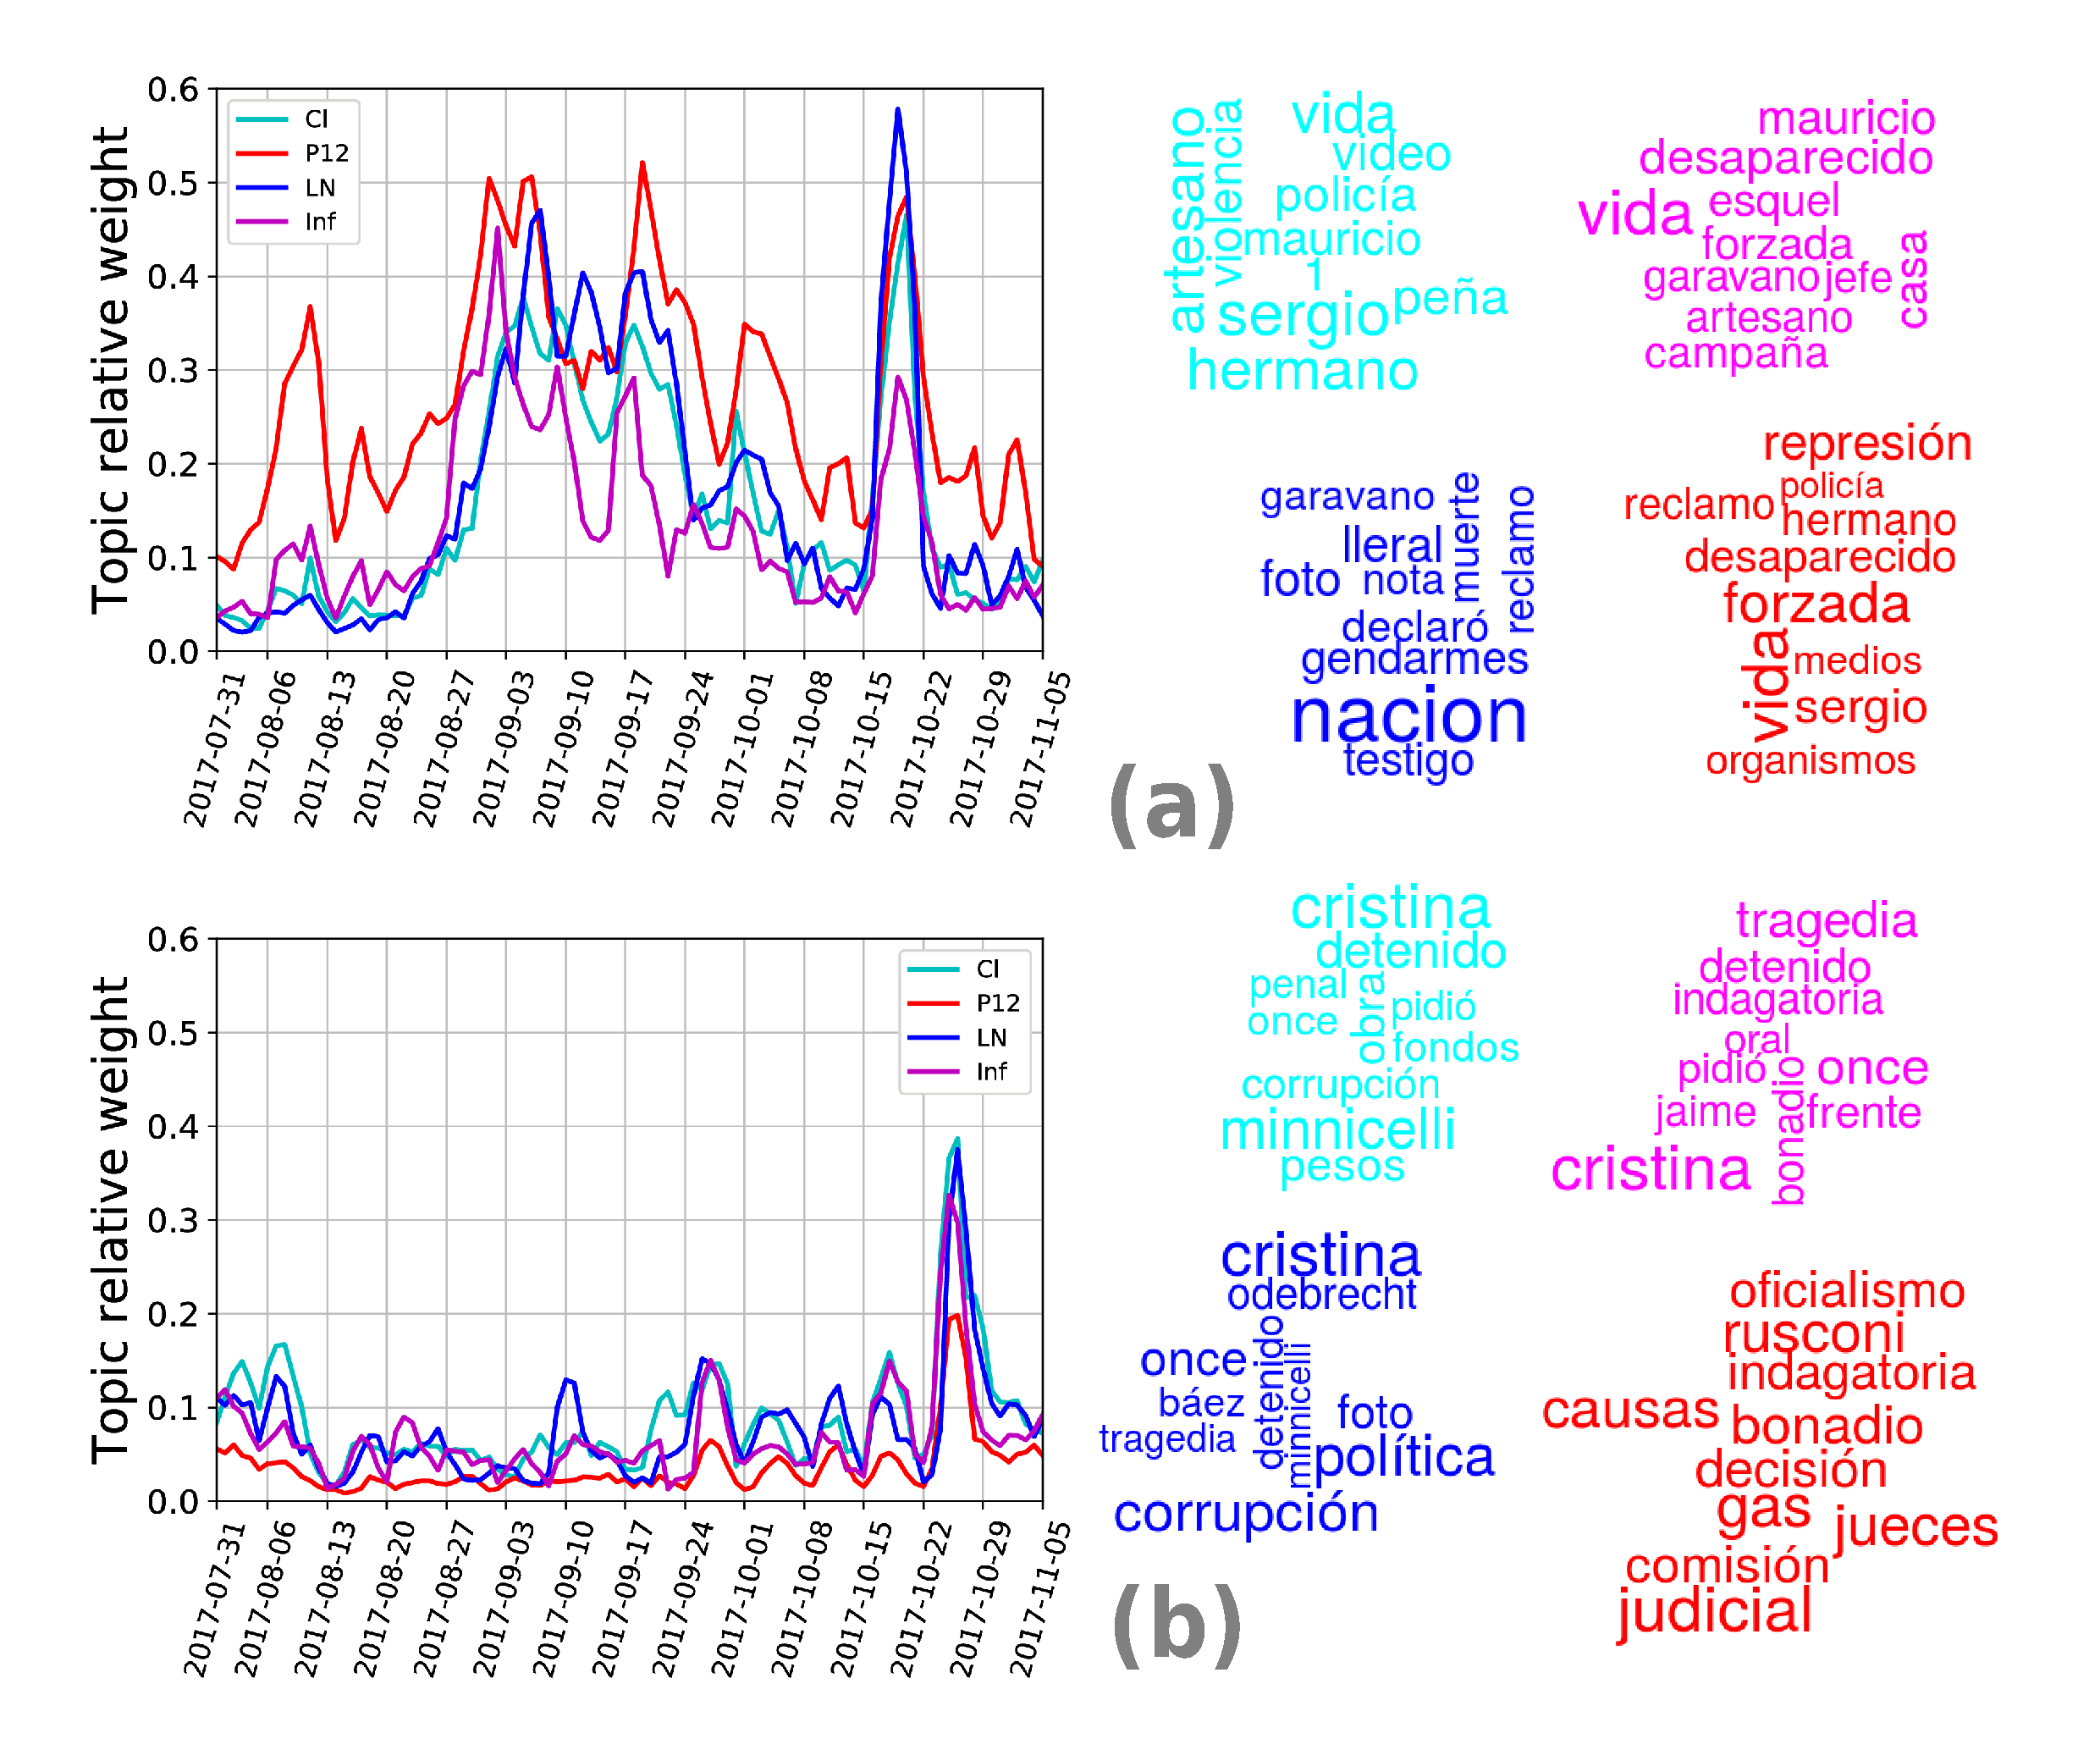
\includegraphics[width = \textwidth]{images/Fig7.pdf}
\caption{\textbf{Relative weight of the topics (a) \emph{Missing person}, and (b) \emph{Former Planning Minister}, and their corresponding word-clouds of frequent newspapers' keywords}. We interpreted the differences shown in given periods as an indicator of coverage bias. For instance, in figure (a) Pagina 12 pays a greater attention in the first days. In the word-clouds, we show which of the defining words are more frequently used by the corresponding newspaper. Most of them are less informative, but other seems to represent a first approximation in the study of framing.}
\label{fig:topics_temporal_profiles}
\end{figure}

\par From panel (a) of figure \ref{fig:topics_temporal_profiles}, we can see the larger coverage of \emph{Pagina 12} respect the other newspapers at the beginning of the period. We can, for instance, quantify this difference calculating  the median of the signals. If we focus in the period between July 31th and August 27th, the median of the topic's relative weight for \emph{Pagina 12} is roughly 0.14 and this is statistically significant larger ($p < 10^{-7}$) than other medians, which are lower than 0.05.
Analyzing the same period, but in panel (b), we again can show that the median in \emph{Pagina 12}, which is roughly 0.01, is lower than the others, which oscillate around 0.05 ($p<10^{-3}$)
This quantification is proposed as method of studying coverage bias in the context of the methodology implemented in our work. 

\par Finally, in figure \ref{fig:topics_temporal_profiles} we also show word-clouds of topic's keywords but separating those who are more frequently mentioned by each newspaper, and filtering the words that are common to all and basically define the factual details of the topic.
Although most of the words are not relevant enough, some of them are quite interesting, as for instance the word \emph{represion} (repression) when \emph{Pagina 12} talks about the topic \emph{Missing Person} and the word \emph{Cristina} (Fernandez de Kirchner, former president) which is employed by all newspapers except \emph{Pagina 12} when they  talk about the topic \emph{Former Planning minister} (see section \ref{sec:Context}).

We think that a more deeply study of topics' keywords could be a first approximation in the study of framing, which will constitute the core of futures works.

\subsection{After all: Who sets the Agenda?}
\label{sec:who_sets}

\par The behavior of the Media Agenda and the Public one, either by looking at Google Trends or Twitter, shows periods when there is a strong similarity among them (mostly in the presence of an unexpected event) and periods when they seem to be unrelated. These are mere observation that talk about the correlation between the agendas.
However the agenda-setting theory is in its nature a theory about causality:vIs the audience a passive actor who follows what the Media says, or there are periods where the Media must paid attention at public's interests?
Paraphrasing the question, who sets the agenda, the Media or the audience?
In a world where social media exists and the feedback between a Media and its audience is common currency, nowadays the idea that the Media sets the agenda and the audience blindly follows it (as it's seemed to be suggested in the original work of McCombs) is too naive.
 
\par In spite of the fact that we think that to establish a causation, i.e. the direction towards information flows, is a task that must be made with extreme care, we have something to say in this work about causality. 
We think that the \emph{Missing person} topic is the most adequate topic to be discussed because:
\begin{itemize} 
\item It caused a great impact in either the Media and the audience
\item  its coverage fully deploys along the time lapse analyzed in this manuscript (see section \ref{sec:Context}).
\end{itemize}

\par In figure \ref{fig:Maldonado_setagenda} we show the topic's relative weight from the Public and Media Agendas.  After the initial coverage, the agendas seem to differentiate around August 16th, when topic started to became more important in the Public Agenda than in the Media one. Around August 24th, the topic abruptly increase in public's interest while the reaction in the Media is slower, showing a significant peak in the plot of the discrete difference (panel (b)) (SEBAS, PODES SENALAR ESTAS FECHAS CON LINEAS PUNTEADAS EN EL GRAFICO?). This date is very close to August 26th, when a campaign in social media took place. After that, the Media increase its coverage about the topic. 

\par Is this a case of reverse agenda-setting, i.e, when the audience set the Media Agenda? 
After all,  the audience get involved about this topic by the Media, so how was the coverage before those events?
By calculating the cumulative sum we can see  the cumulative coverage during the first events related to the topic. 
This measure can be seen as the numerical integrate of the temporal profiles of figure \ref{fig:topics_temporal_profiles} between the initial date and the current date. 
It is interesting to note that the newspaper responsible to accumulate coverage during the initial stage was the minority one: \emph{Pagina 12}. 

Our interpretation about the setting agenda dynamics of this particular topic is the following: A small newspaper (\emph{Pagina 12}) gives great coverage to this topic; it is amplified  by public in the social networks and also expressed  by reiterative Google searches. Then the rest of the Media  pay attention to this subject and it becomes an important topic in the Media Agenda. 
This interpretation try to catch in a qualitative way how the information flow was in this specific topic.
On the other hand, behind this interpretation there are two important facts that must be mentioned: First, the disappearance of a person is a very sensible theme for the Argentinian society, and second, there are political reasons in why \emph{Pagina 12} was particularly interested in cover this topic while the other Media did not follow this interest.

\par We took the question about causality only in a qualitative way. 
There are different metrics that would help in this question, such as Granger causality or correlation by sliding windows. We think that this analysis must be performed with extreme care since the acquirement of the data.
With this work we aimed to provide a quantitative characterization of the behavior of the Media and the Public but not to establish direction of causation, which we hope this to be the core of future ones.


\begin{figure}
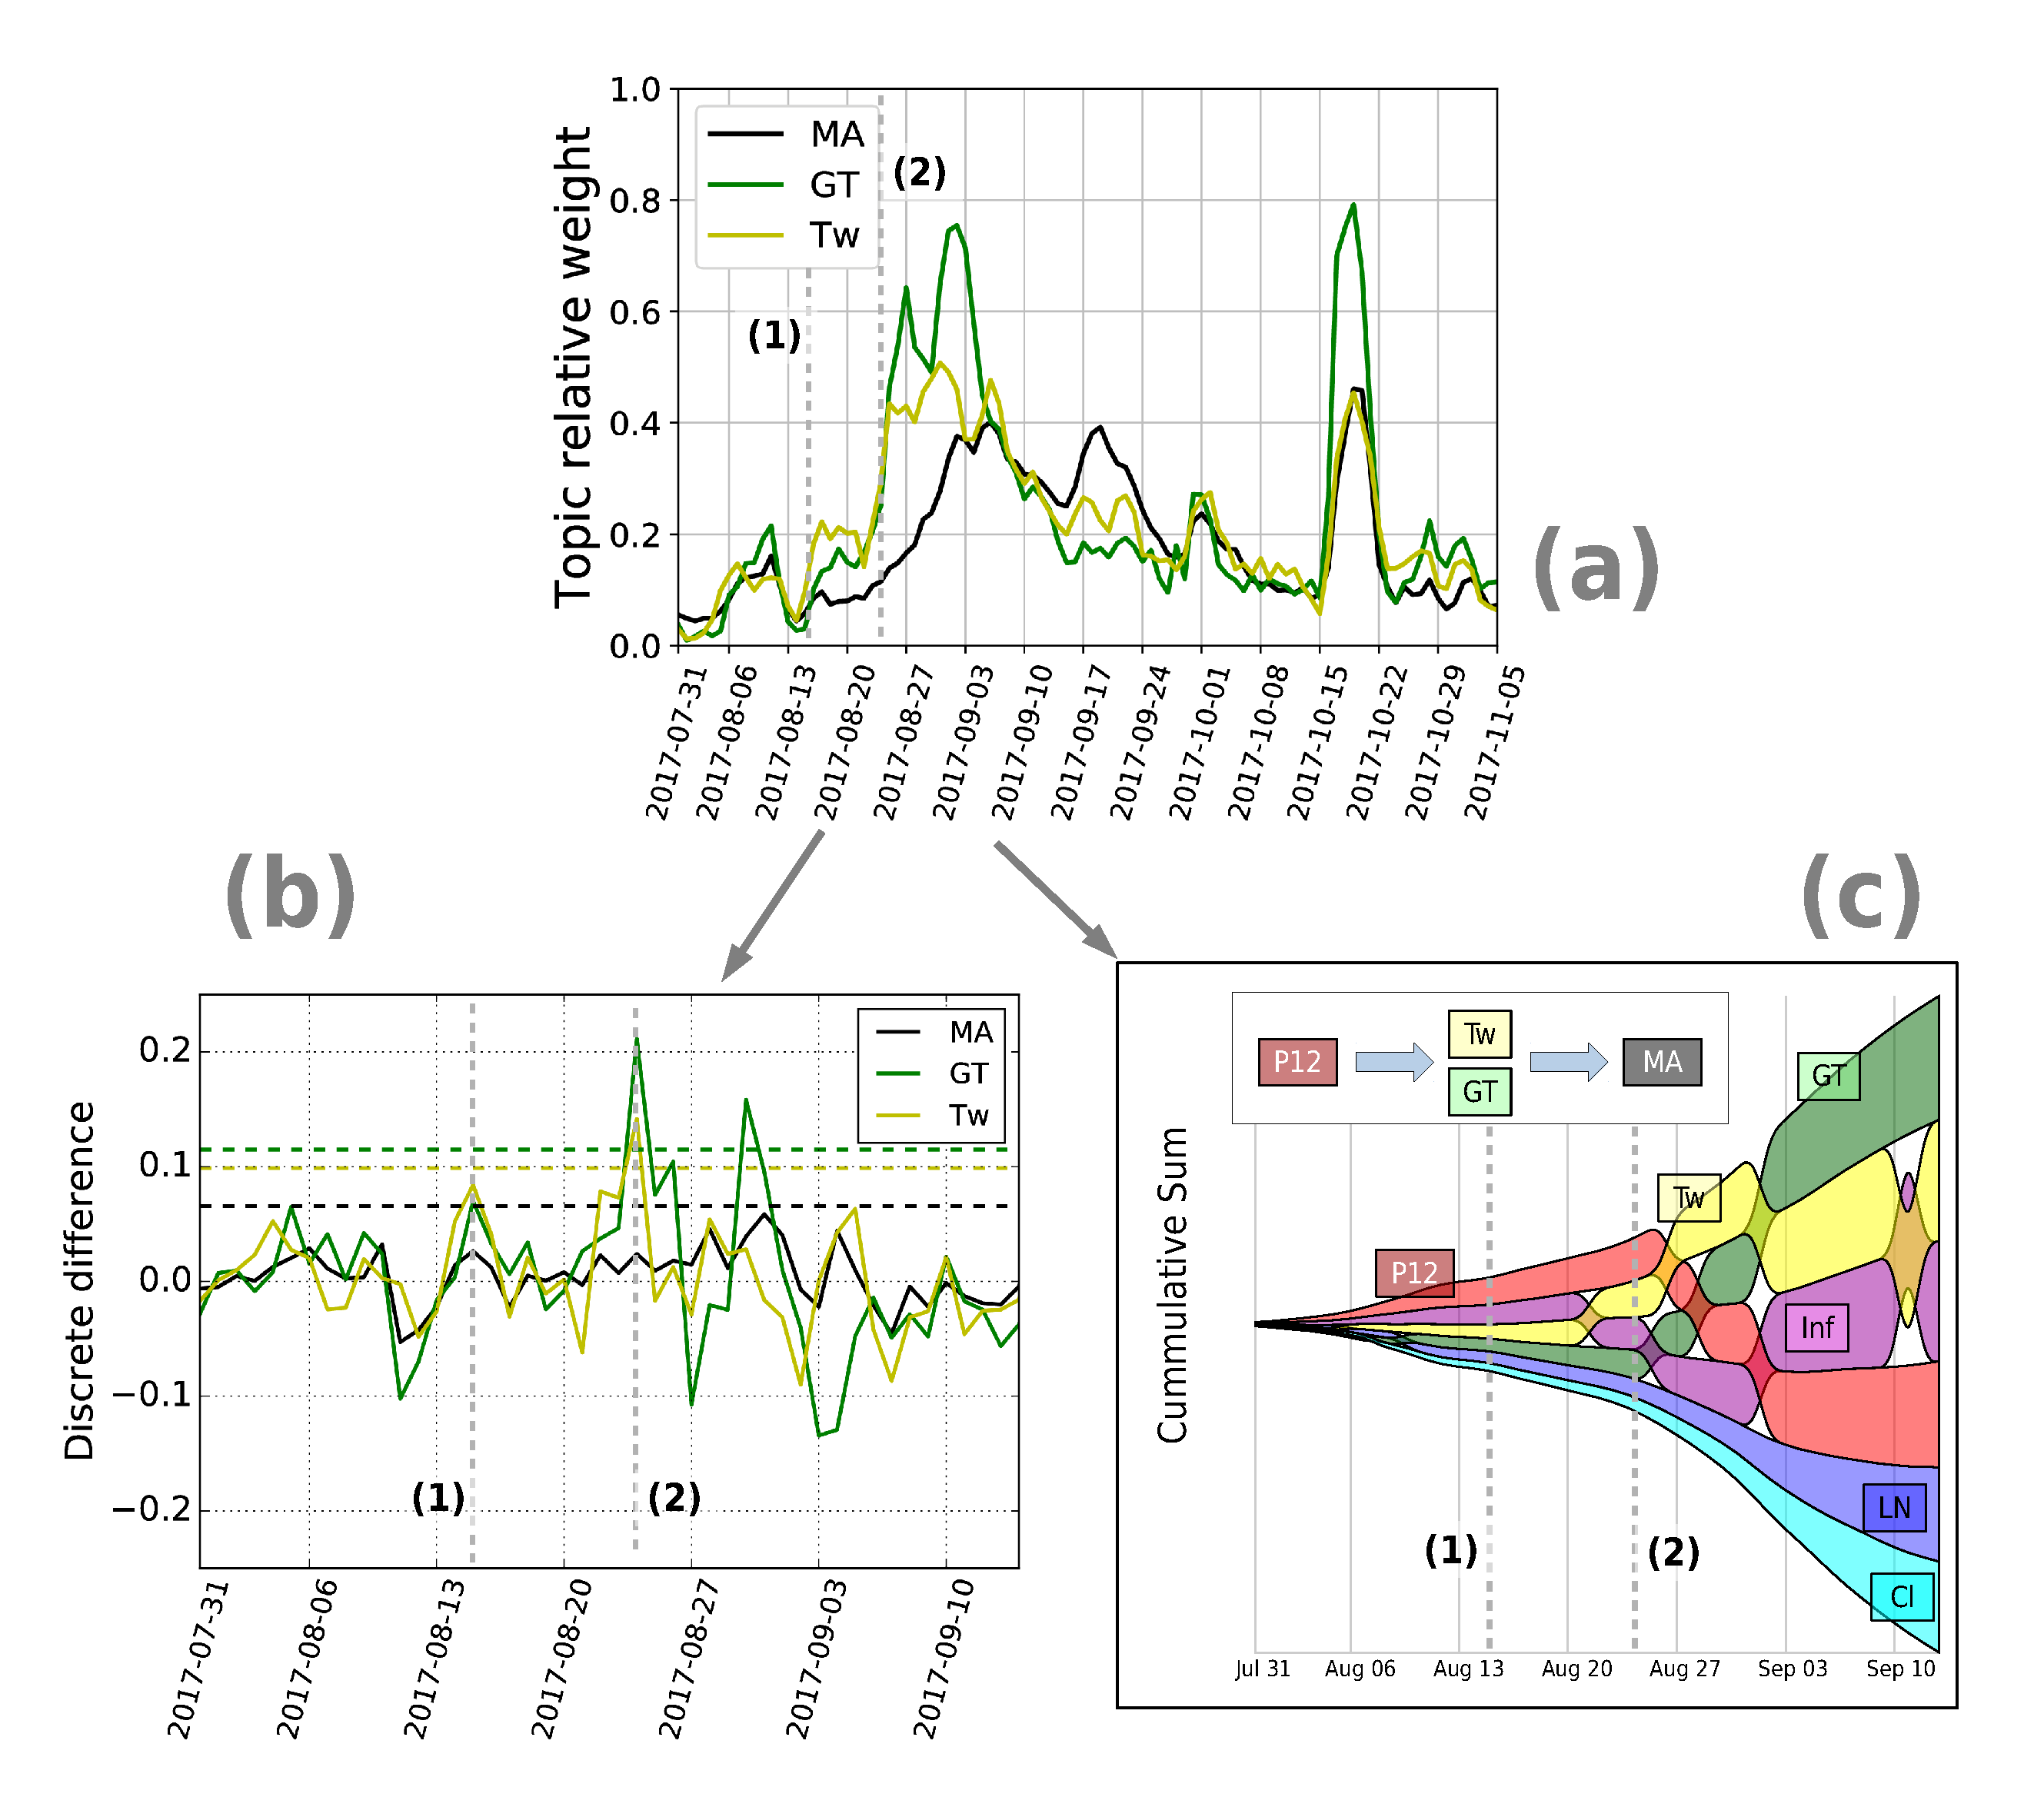
\includegraphics[width = \textwidth]{images/Fig8.pdf}
\caption{\textbf{Agenda setting direction in Missing person's topic?}
The temporal profiles of figure (a) show that the Public increased abruptly its interest in the topic around August 24th, which belongs to the peak \textbf{(*)} shown in figure (b), where the discrete differences were computed. 
This date is also pointed out in the rest of the figures with a vertical grey line together with the asterisk. 
With the computing of the cumulative sum of figure \ref{fig:topics_temporal_profiles} and figure (a), represented as a bump chart in figure (c), we suggest that the topic was first set by \emph{Pagina 12} and then the Public's interest cause the coverage of the other Media.
}
\label{fig:Maldonado_setagenda}
\end{figure}

%\section{Conclusions}

\par The study of Mass Media, and in particular the agenda setting theory, can be empowered by the used of data mining or machine learning algorithms. 
In this work, through the implementation of a topic detection algorithm we could describe the Agenda of the Media as a distribution which evolves over time and which is defined in a topic's space which emerges from the analysis of the corpus.
This gave us an insight of how we can construct and follow the Public's interests, the Public Agenda, in order to compare with the Media Agenda, i.e. Media interests. 
\par Given the Agendas, we found that the Public one is usually less diverse than the Media, showing that when there is a very attractive topic, the audience focus on this one, when the Media has to cover the other too. 
On the other hand, the measurement of distances between Agendas can be employed to rapidly detect periods when the Public may have an independent behavior respect to the Media. The methodology implemented here also allow us to detect coverage bias in newspapers and gave us a first approximation in the theory of framing. 
\par We hope that some of the elements studied here will give us insights at the time of proposing a mathematical model about Mass Media and Public interaction. Future works may include a more systematic study and its extension to international Media, a deeper study of framing through topic detection and sentiment analysis, and a more quantitave analysis about causation.

\section{Conclusions}

\par The study of Mass Media, and in particular the agenda setting theory, can be empowered by the used of data mining or machine learning algorithms. 
In this work, through the implementation of a topic detection algorithm we could describe the Agenda of the Media as a distribution which evolves over time and which is defined in a topic's space which emerges from the analysis of the corpus.
This gave us an insight of how we can construct and follow the Public's interests, the Public Agenda, in order to compare with the Media Agenda, i.e. Media interests. 
\par Given the Agendas, we found that the Public one is usually less diverse than the Media, showing that when there is a very attractive topic, the audience focus on this one, when the Media has to cover the other too. 
On the other hand, the measurement of distances between Agendas can be employed to rapidly detect periods when the Public may have an independent behavior respect to the Media. The methodology implemented here also allow us to detect coverage bias in newspapers and gave us a first approximation in the theory of framing. 
\par We hope that some of the elements studied here will give us insights at the time of proposing a mathematical model about Mass Media and Public interaction. Future works may include a more systematic study and its extension to international Media, a deeper study of framing through topic detection and sentiment analysis, and a more quantitative analysis about causality.


%
\section{Discussion}


\par As was mentioned above, the starting point of our analysis is the topic decomposition of the corpus.
We chose to decompose the corpus in 10 topics, which three of them we interpret to be talking about the same macro-topic which we called \emph{Elections}, while other two were intereted as talking about other macro-topic called \emph{Missing person}, as can be seen below. 
The meaning of the topics or macro-topics are more explained in section \ref{sec:Context}. 
So the final description of the agendas is made with only 7 topics.
We opted for choosing this arbitrary number of topics in order to describe the corpus with as least information as possible, but it is not more than an arbitrary decision, validated in some manner by our knowledge of the corpus.
After the proceedings describe in section \ref{sec:Methodology}, we construct the \textbf{Media Agenda (MA)} and the \textbf{Public Agenda (PA)}, and all their derivations, as time-dependent distributions. 

\subsection{Media and Public agenda: a qualitative approach}

\par In figure \ref{fig:topics_wordclouds} we show the radar plots of the average distributions of the \textbf{MA} and the \textbf{PA} discriminated by \textbf{GT} and \textbf{Tw} together with the introduction of the topics' names.
A radar plot is an alternative of histograms that allows the visual comparison of distributions easier.
In this figure we also show the wordclouds of the keywords that define each topic, where the size of the word belongs to the importance in the topic's definition given by the topic detection algorithm. In green color, we point out the words involved in the Google Trends and Twitter queries in order to construct the Public Agenda. The queries employed are also specified in table \ref{table:gt_all_correlation} together with the linear correlation between the topics' temporal profiles that form the Public Agenda and their counterparts in the Media Agenda.

\par On the other hand, in figure \ref{fig:all_agenda} we show a bump chart of the Agendas, which is the dynamical representation of the Agendas of figure \ref{fig:topics_wordclouds}. 
A bump chart provides us a very useful visualization tool for displaying the relative weight of the topics and at the same time their ranking, putting on the top the most important topic at a particular date.
In figure \ref{fig:all_agenda} we also point out some important events related to the topics.

% Wordclouds
\begin{figure}[h]
\centering
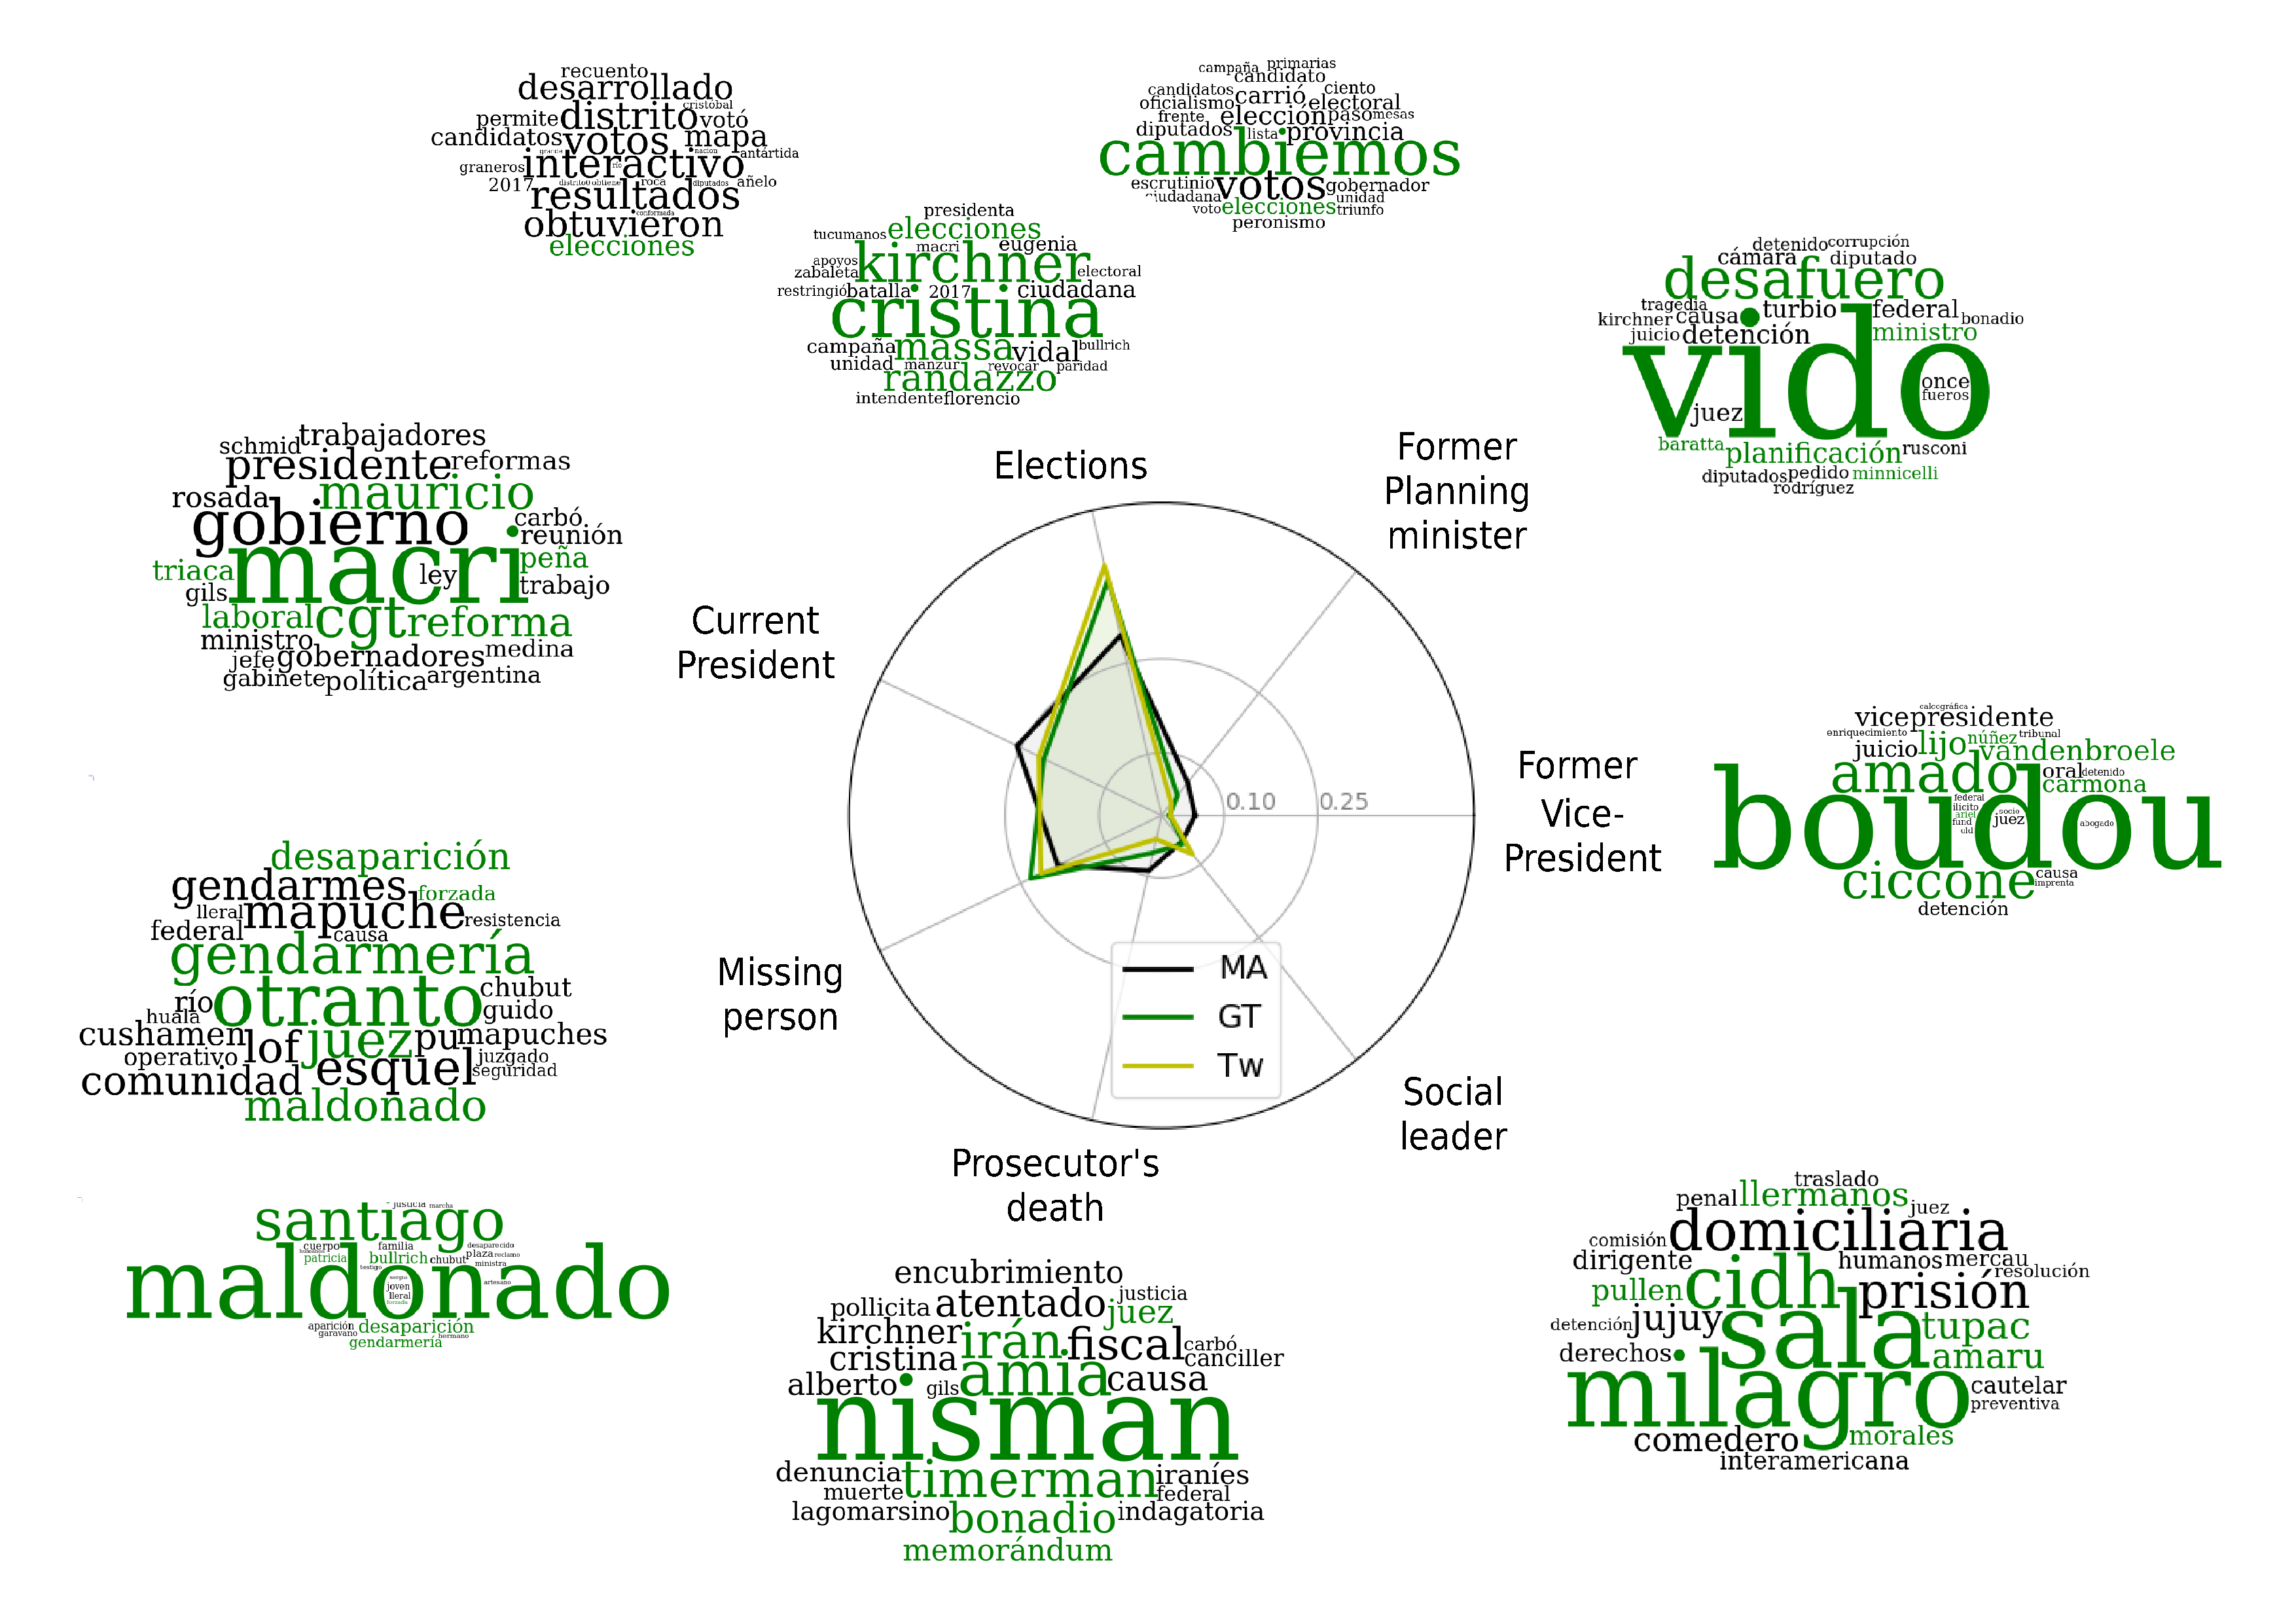
\includegraphics[width = \textwidth]{images/Fig1.pdf}
\caption{\textbf{Radar plots of the Media and Public Agenda average distributions and topics' wordclouds.} The Public Agenda is represented either by Google Trends (Gt) and Twitter (Tw). 
Topics’ names are introduced together with the wordclouds containing the most important keywords involved in the definition of each topic.
In green color we show those included in the Google Trends and Twitter queries (see table \ref{table:gt_all_correlation}) and therefore in our construction of the Public Agenda.
}
\label{fig:topics_wordclouds}
\end{figure}


% Global Agenda figure!!!
\begin{figure}[h]
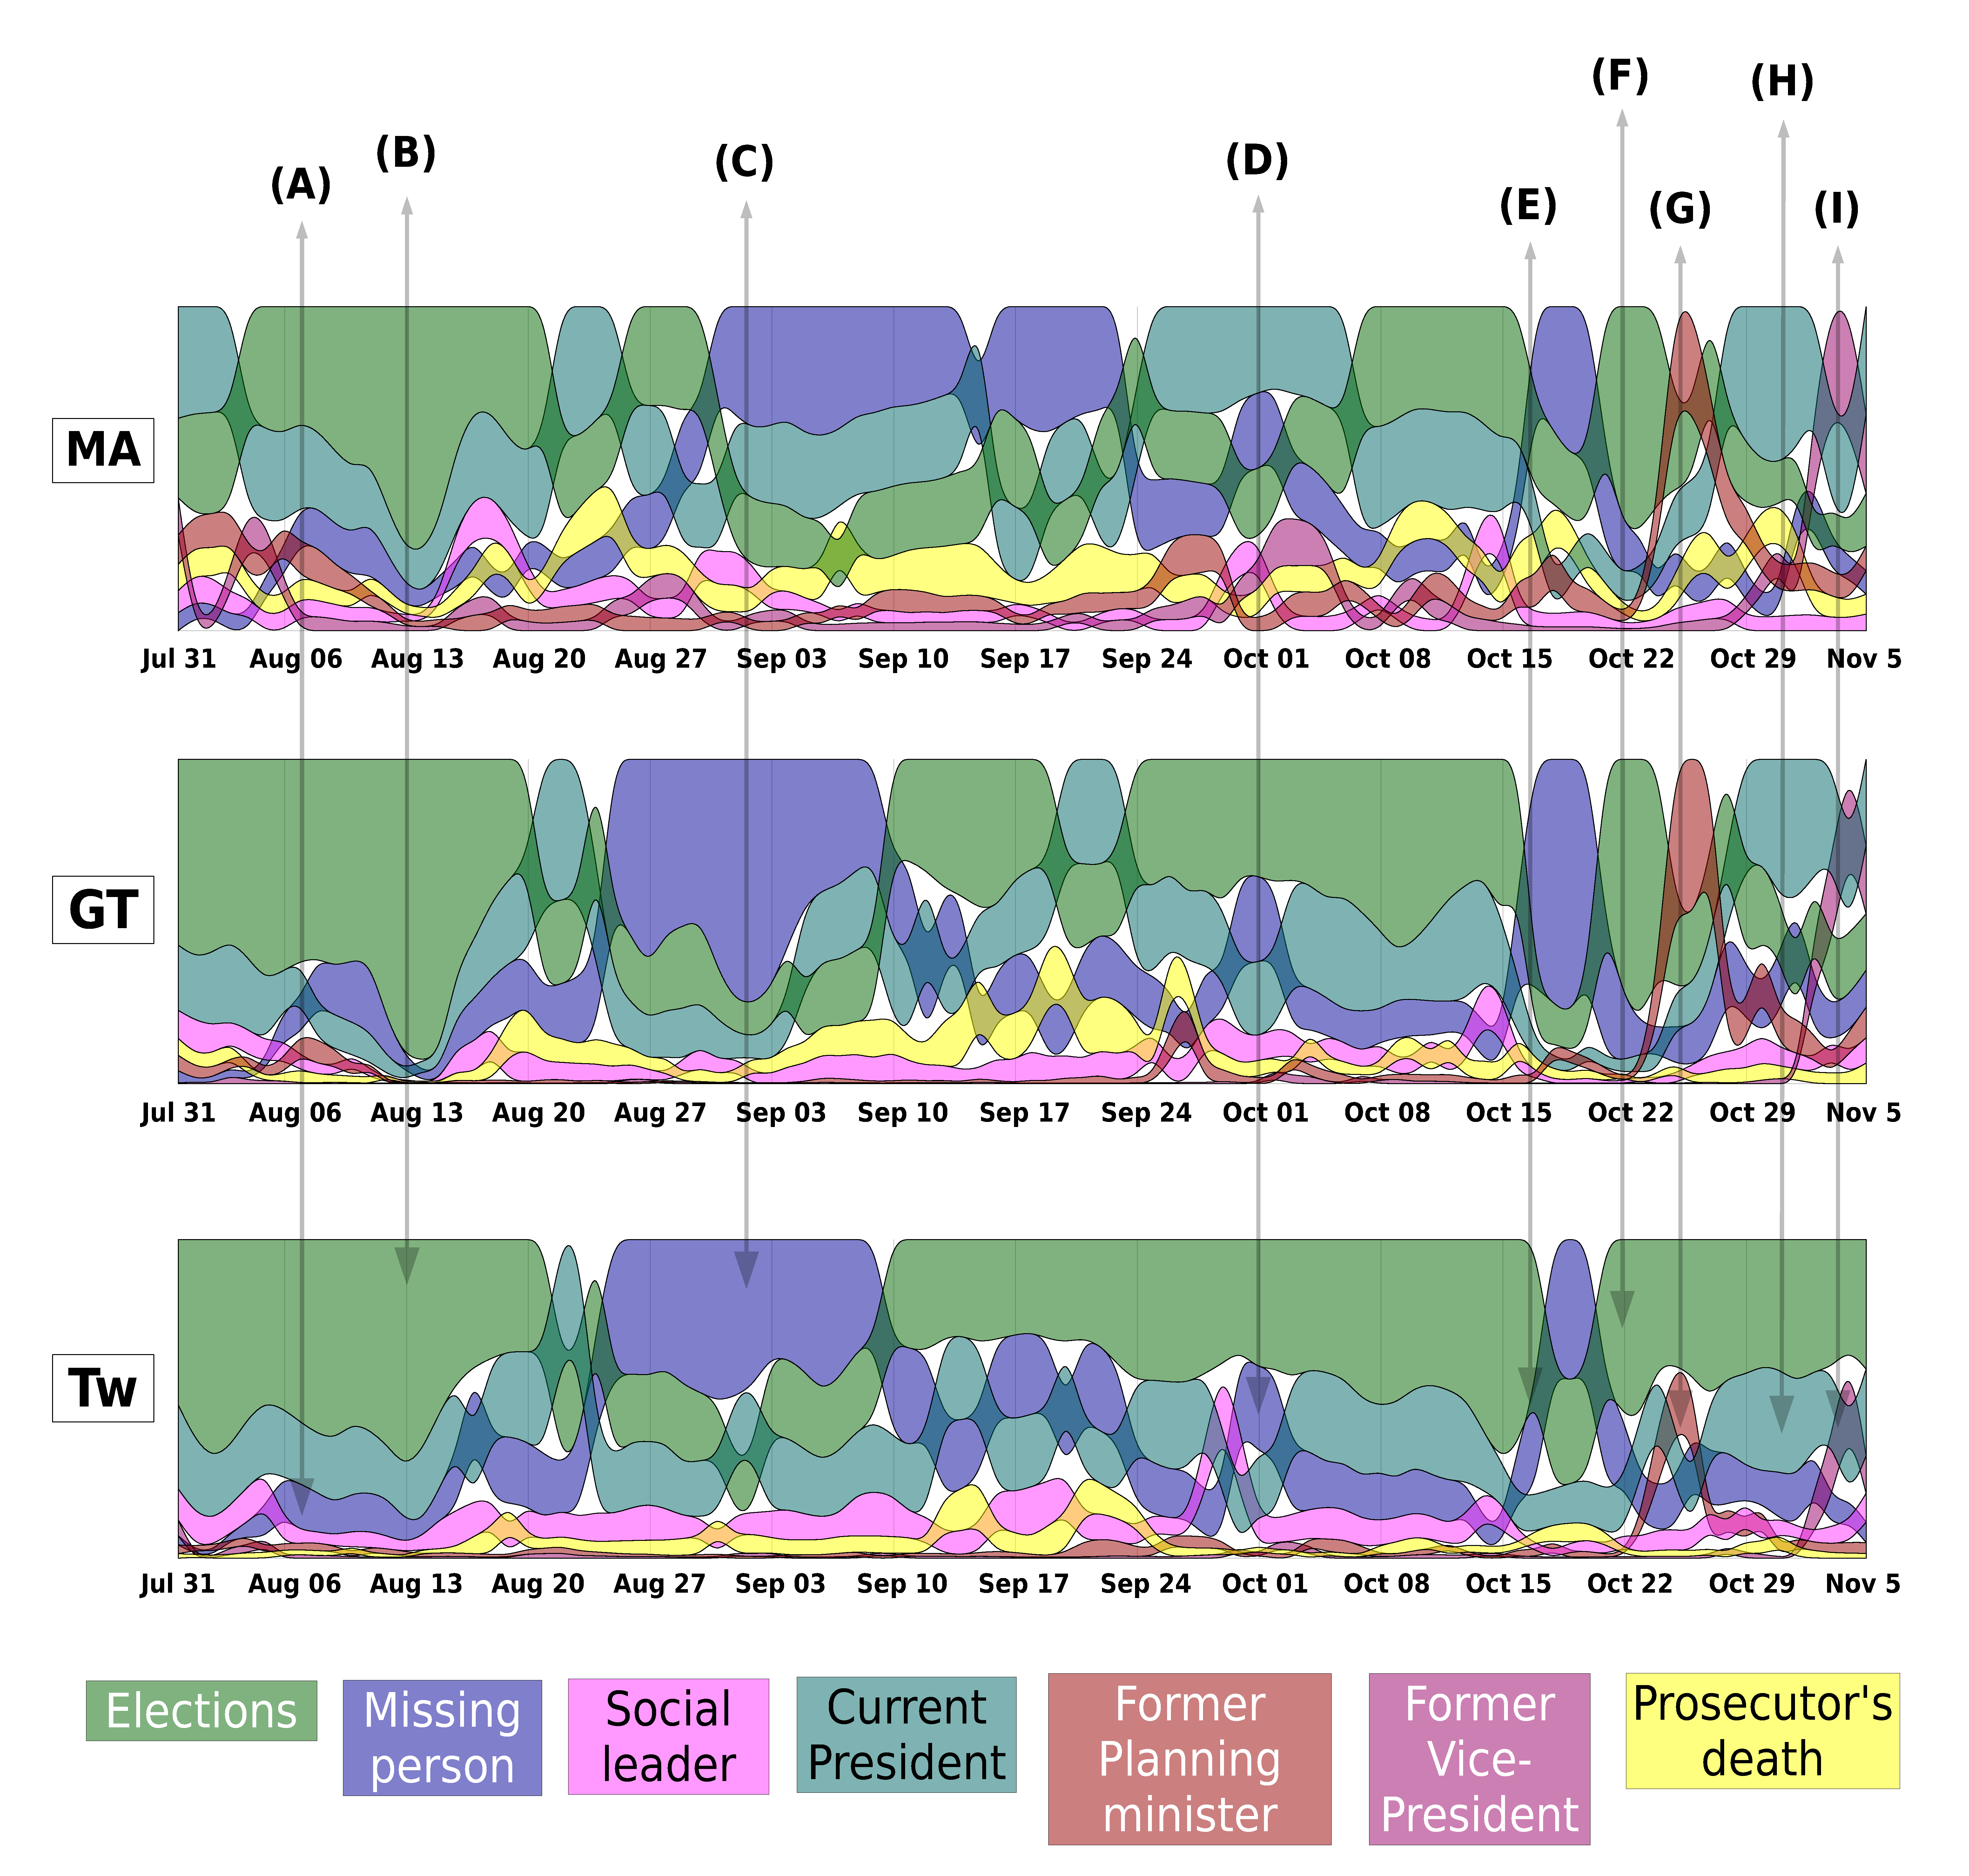
\includegraphics[width = \textwidth]{images/Fig2.pdf}
\caption{\textbf{Bump graph of the Media Agenda (MA) and Public Agenda extracted from Google Trends (Gt) and Twitter (Tw).} Some important events related to the topics are pointed out. The curves’ width and their ordering are related to the topics’ relative weight.}
\label{fig:all_agenda}
\end{figure}
 

\footnote{Due to different characteristics in the search tool of Twitter, we adapted the queries employed here but preserving the at least at we can the most important keywords. The queries employed by topic were: \\
Elections: elecciones + cambiemos + kirchner + massa + randazzo \\
Missing person: maldonado + otranto + gendarmeria + desaparicion \\
Former Planning minister: vido + desafuero + minnicelli + baratta \\
Current President: macri + cgt + laboral +  triaca \\
Social leader:  sala + cidh + tupac + amaru + pullen + llermanos + morales \\
Prosecutor’s death: nisman + amia + memorandum + timerman +  bonadio \\
Former Vice-President:  boudou + ciccone +  lijo + vandenbroele + carmona
}

% Table with queries and correlations
\begin{table}[h]
\centering
\resizebox{\textwidth}{!}{\begin{tabular}{llccc}
\toprule
& Google Trends query & Correlation MA and Gt & MA and Twitter & Gt and Twitter \\ 
\midrule
Elections & elecciones + cambiemos + cristina kirchner + massa + randazzo & \textbf{0.81} & \textbf{0.59} & \textbf{0.75} \\
Missing person & santiago maldonado + juez otranto + patricia bullrich + gendarmería + desaparición forzada & \textbf{0.68} & \textbf{0.76} & \textbf{0.89} \\
Former Planning minister & de vido + desafuero + ministro de planificación + minnicelli + baratta & \textbf{0.92} & \textbf{0.82} & \textbf{0.87} \\
Current President & mauricio macri + cgt + reforma laboral + peña + triaca & \textbf{0.77} & \textbf{0.75} & \textbf{0.63} \\
Social leader & milagro sala + cidh + tupac amaru + pullen llermanos + morales & \textbf{0.49} & \textbf{0.25(*)} & \textbf{0.57} \\
Prosecutor's death & nisman + amia + memorándum con irán + timerman + juez bonadio & \textbf{0.56} & \textbf{0.59} & \textbf{0.75} \\
Former Vice-President & amado boudou + ciccone + ariel lijo + vandenbroele + núñez carmona & \textbf{0.90} & \textbf{0.92} & \textbf{0.97}\\
\bottomrule
\end{tabular}}


\caption{Queries performed in Google Trends in order to made up the Public Agenda. 
We also shown the correlation between the topics' temporal profiles of the Public Agenda and their counterpart in Media Agenda.
All correlation values are statistical significant ($p < 10^{-9}$), except (*) which is significant with $p < 0.05$.}
\label{table:gt_all_correlation}
\end{table}


\par The figures introduced above show in a qualitative way the differences between the agendas, and the dynamics of the topics, i.e. the range of dates in which a given topic was an important one, for which topic it was replaced, and so on. 
We can see, for instance in the radar plot of figure \ref{fig:topics_wordclouds}, a more interest of the audience in the topic \emph{Missing person} than the Media, or inversely in the topic \emph{Prosecutor's death}, when we see all the period analyzed as a whole. 
Also we can observe a great similarity between \textbf{Gt} and \textbf{Tw} agendas which form the Public Agenda.
\par On the other hand, the linear correlations of table \ref{table:gt_all_correlation} are in all cases positive and statistically significant, which we interpret as a form of validation of the topics found in the corpus and the keywords that describe it. 
We expected that the Media's and public's interest should generally follow a similar a pattern due to the external events, although the periods where those differ are of particular interest for us. 
A non positive (or a non significant) correlation may imply that we are not properly detecting the keywords or features that describe a particular topic, so the Google Trends' or Twitter's pattern would not be able to reflect a similar behavior that its counterpart in the Media.


\subsection{A quantitative approach}

\subsubsection{Agenda diversity}

% Agenda diversity

\par In order to quantify the similarities and differences between the Media Agenda and the Public Agenda, we start by asking how is the distribution of each agenda among the topic's space. In particular, we measure how diverse is each agenda. Following \cite{boydstun2014importance}, we calculate the normalized Shannon's entropy ($H$, see eq.\ref{eq:shannon_entropy}) in order to measure the diversity of the \textbf{MA} and \textbf{PA}.
\par In figure \ref{fig:shannon_entropy_agendas} we can see the value of $H$ as a function of time. We can see that there are periods where the diversity is lower than the usual, more notorious in the Public Agenda giving by \textbf{Gt}. 
We are going to pay attention to four dates in the Public Agenda, which three detected as outliers of the typical behavior, two from \textbf{Gt} and one from \textbf{Tw}. 
\par A small value in the diversity is due to the fact that the most important topic attracts practically all the attention of the public or the media.
In the radar plots included also in figure \ref{fig:shannon_entropy_agendas} we can see that two of the points (\textbf{a} and \textbf{d}) belong to the topic \emph{Elections} and coincide with the primary and general legislative elections that took place in August 13th and October 22th. 
In all the agendas these points where detected as outliers except point (d) in Twitter Agenda: By inspecting the radar plot the diversity in this agenda can be the result of the association between the topic \emph{Elections} and the \emph{Current President}.
Discussions in Twitter about elections appear also in point (c), when the other agendas seems to be more diverse. 
On the other hand, we inspect the point (b) despite not being detected as a outlier, which belong to the topic \emph{Missing person} and related to a month after the disappearance of Santiago Maldonado (see section \ref{sec:Context}). 
We emphasize the discussion about this topic because we see interesting facts that appear along the analysis.

\begin{figure}[h]
\centering
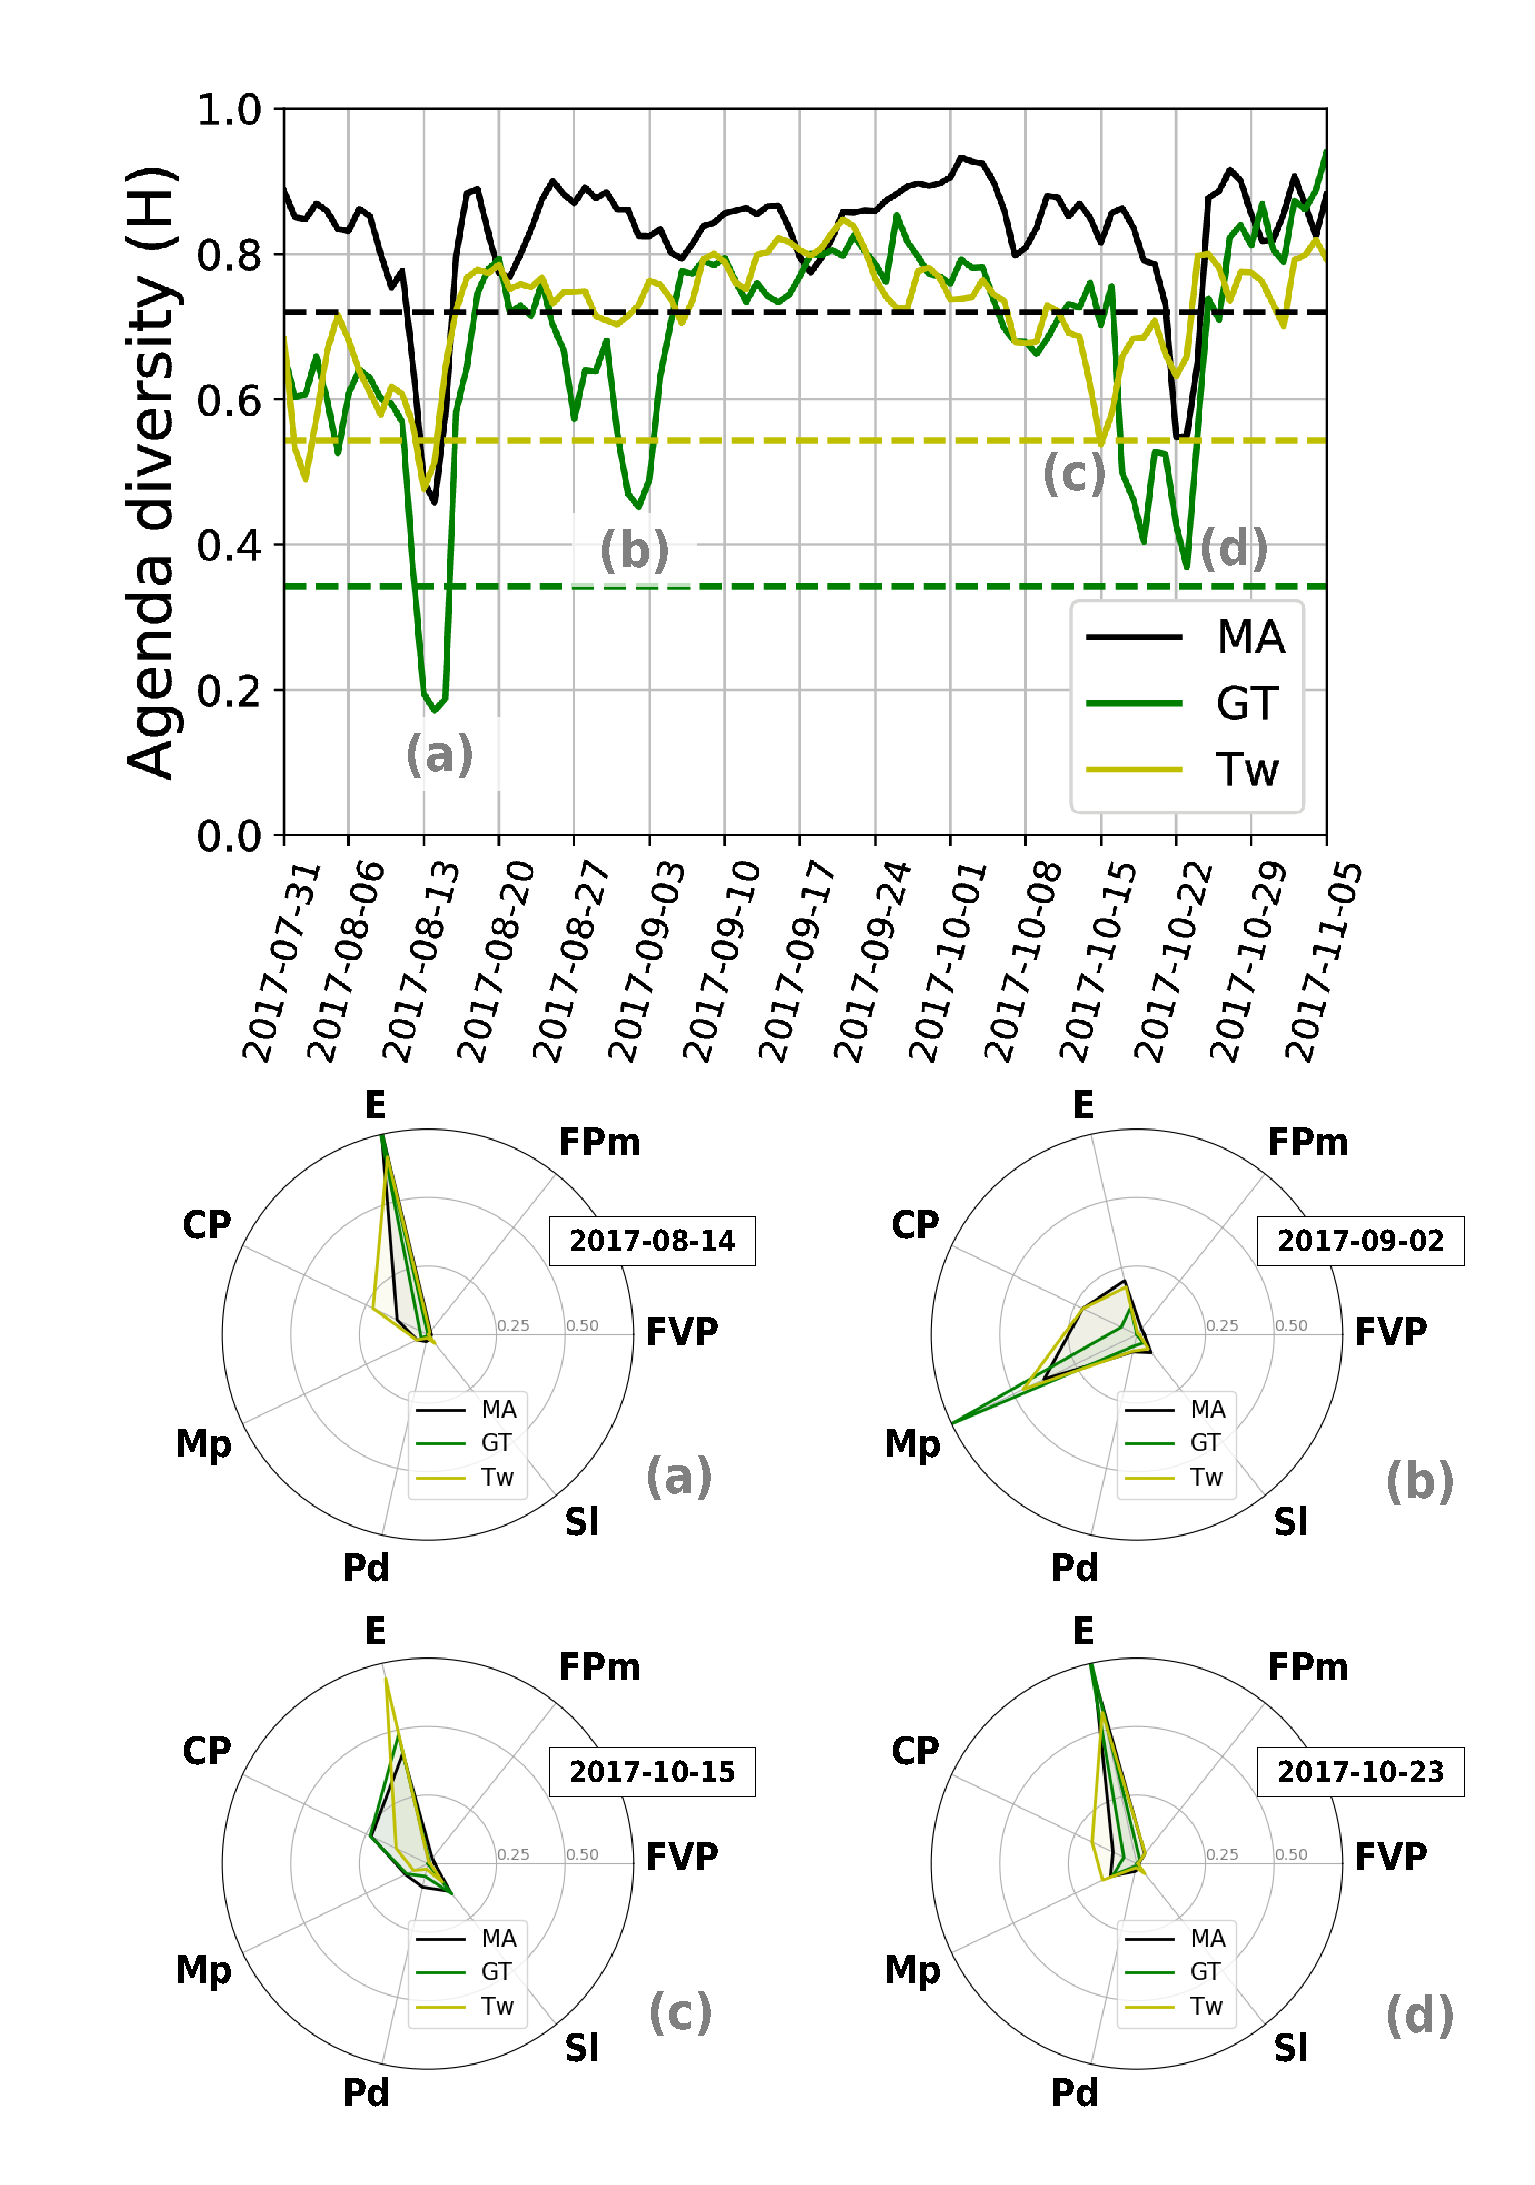
\includegraphics[width = \textwidth]{images/Fig3.pdf}
\caption{\textbf{Shannon entropy (H) as a measure of agenda diversity.} The Public Agenda show a less diverse behavior than the Media Agenda as can be seen in the left figure. The horizontal lines are the lower inner fences of each signal in order to identify outliers. The related radar plots shows that those dates when the agenda has a low diversity, the most important topic catches the most public’s attention}
\label{fig:shannon_entropy_agendas}
\end{figure}

\par From the measure of $H$ we can also see that the median of the Public Agenda diversity is statistical significant lower than the Media Agenda's one.
Specifically $H_{Gt} = 0.73$ and $H_{Tw} = 0.74$ are statistical significant lower than $H_{MA} = 0.85$ with $p < 10^{-18}$, while there is no significant difference between the first two. 
However from figure \ref{fig:shannon_entropy_agendas} we can see that \textbf{Gt} shows more abrupt falls in the diversity in response to specific events.
We conclude that its an important fact about audience behavior: given a finite set of topics, \textbf{the Public Agenda is less diverse than the Media Agenda}, because the public seems to focus more in the most important topic than the Media can do, maybe due to editorial decisions.

\subsubsection{Public Agenda's distance}

% Jensen-Shannon distance between PA and MA

\par The measurement of the Shannon's entropy made above is an independent property of each distribution. 
Here we directly compare the Agendas by computing the Jensen-Shannon distance. We again identify outliers and aim to interpret them.
In figure \ref{fig:jensen_shannon_gt} we show the Jensen-Shannon distance as a function of time. We inspect three points that seems to be of particular interest. In all cases, the radar plots shows that a greater distance is associated with a more interest of public in the topic \emph{Missing person}. 
\par Points \textbf{(c)} and \textbf{(d)} shows that both the public and the Media are interest in that topic, but the Media have to cover other topics, so the distance value can be seen as a derivation of the diversity effect discussed in the last section.
However points \textbf{(a)} (we take this point due to be a extreme of the distance in the middle of the period despite not being an outlier) and \textbf{(b)} seem to show an interest of the public in the topic \emph{Missing person} which it is not reflected in the Media. 
In figure \ref{fig:all_agenda} we can see that this topic reached the first place in public's interest in both \textbf{Gt} and \textbf{Tw} before that in the Media. We associate this fact with a campaign made in social media like Facebook and Twitter in August 26th, that paid for the appearance of Santiago Maldonado and had a great repercussion, maybe at first underestimated by the Media (see section \ref{sec:Context}). 
\par It is important to recall that it is our interpretation based on the knowledge of the context, and that we are not studying causality (we will say a few words about it in section \ref{sec:who_sets}), i.e. we can't say, for instance, that in this case the Public Agenda set the Media Agenda. 
However, the Jensen-Shannon distance, in conjunction with the measurement of the agenda diversity given by the Shannon entropy, give an insight of independent behavior of the Public and the Media, and its identification can be a starting point to study the Media reaction to a change in audience's interests.
 
\begin{figure}[h]
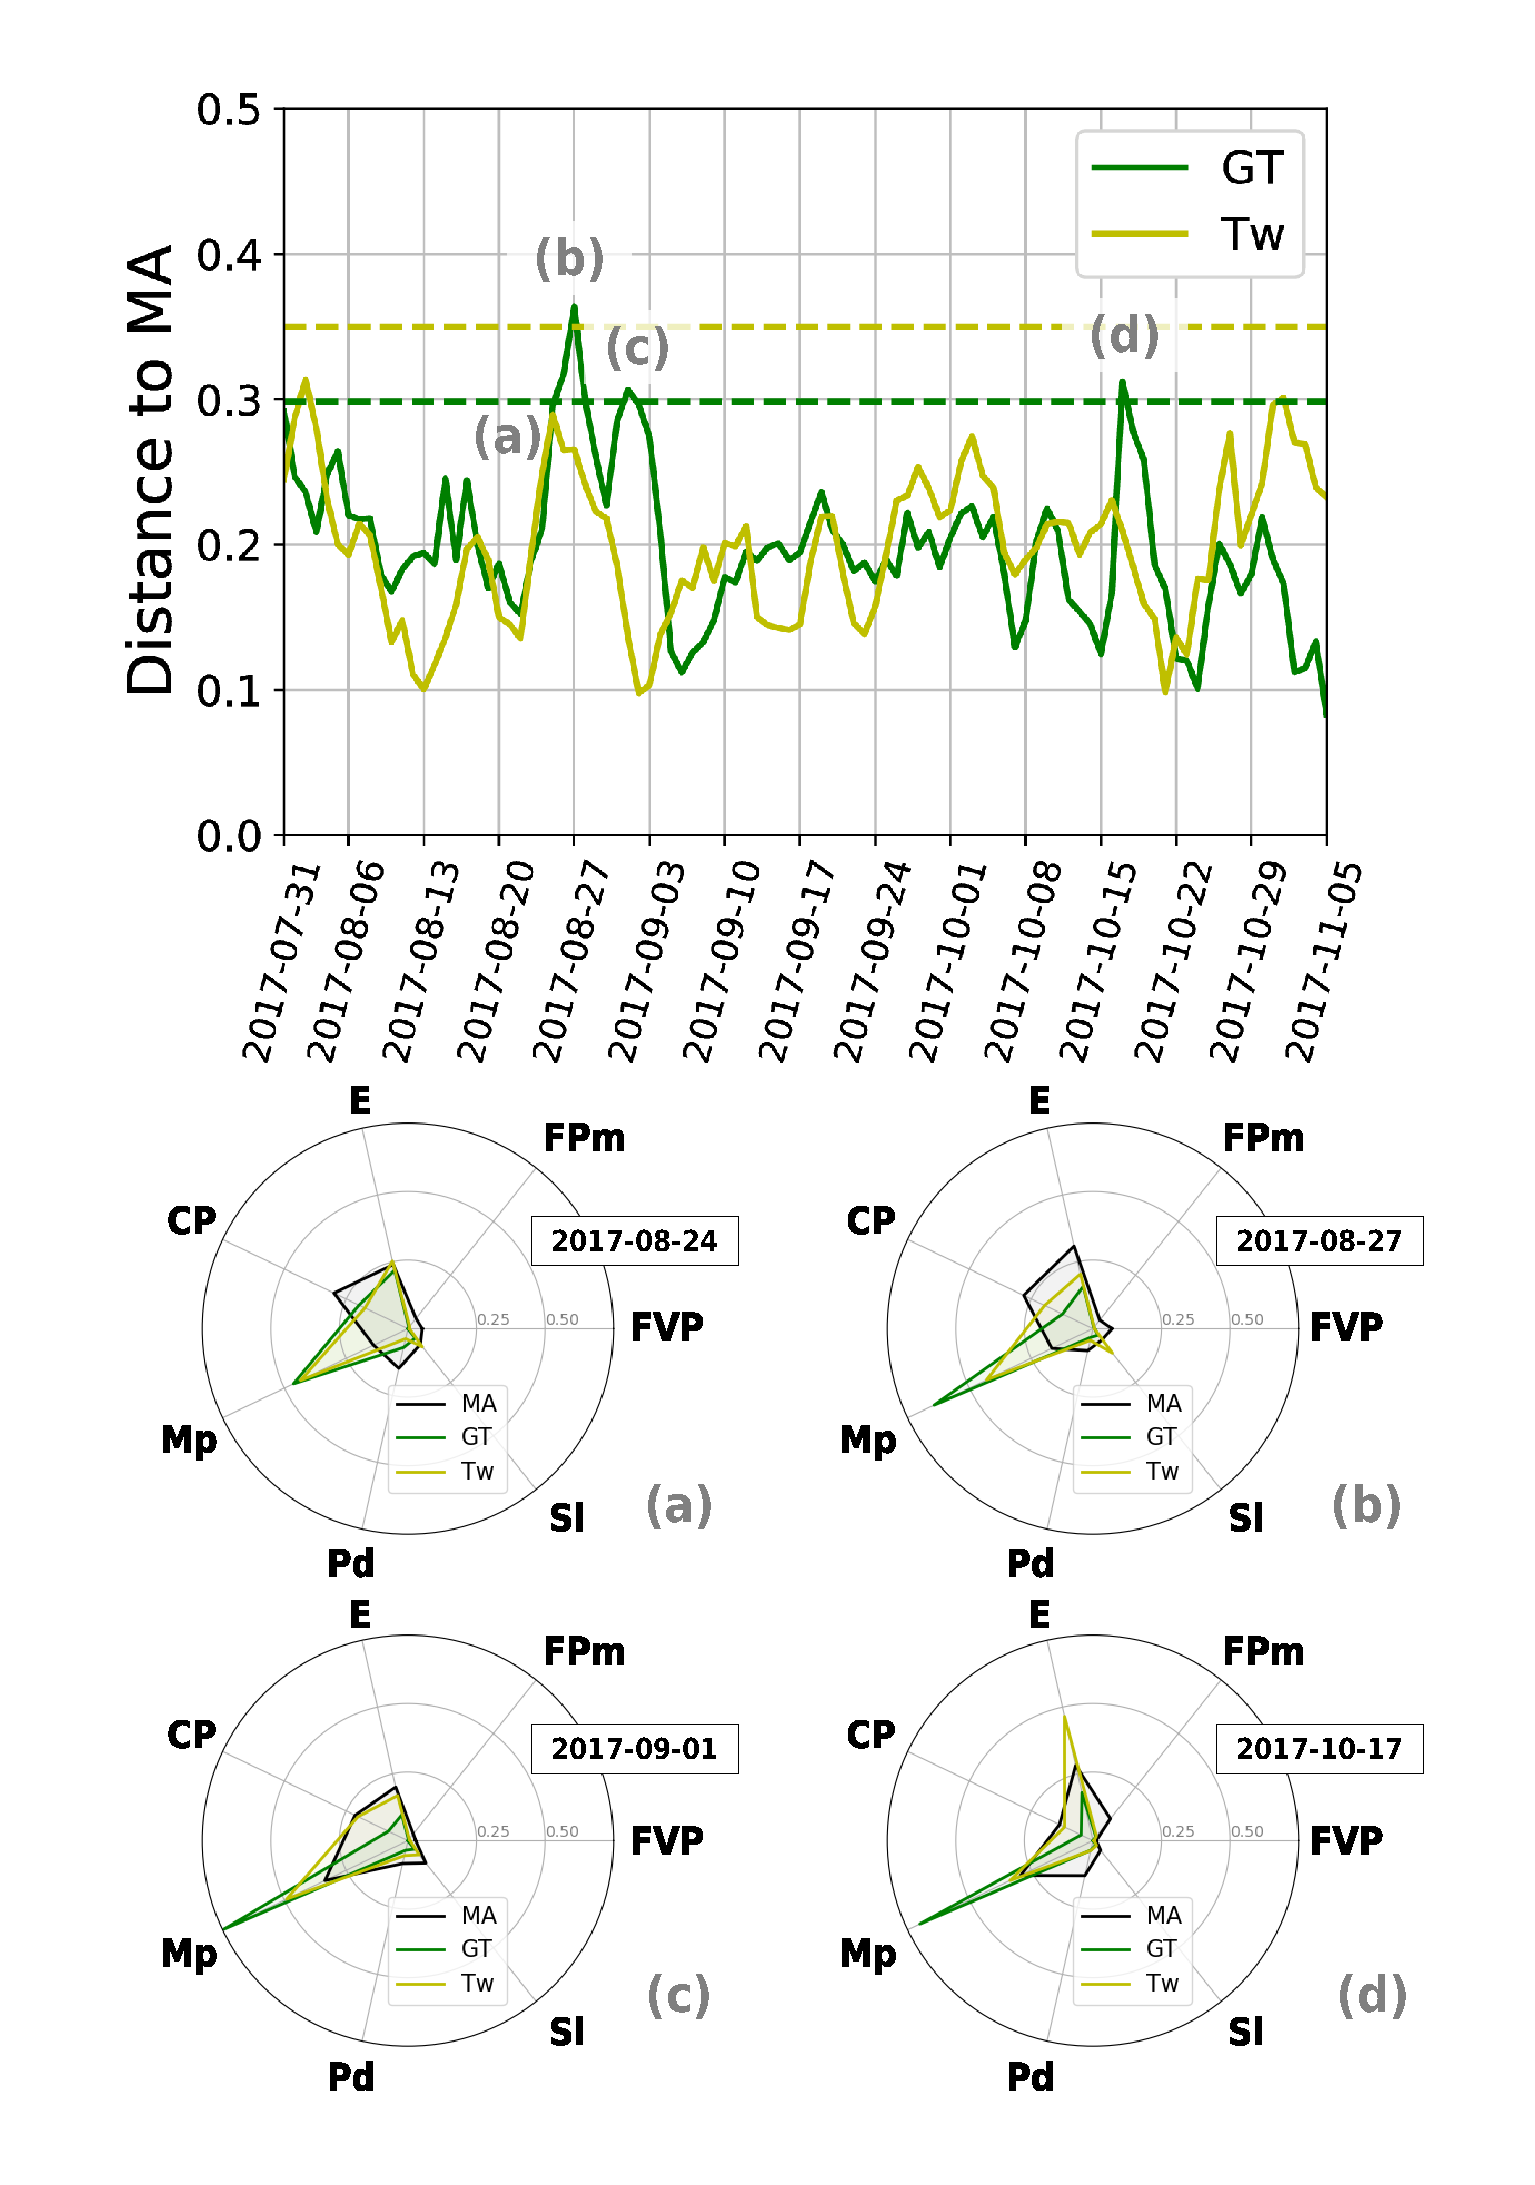
\includegraphics[width = \textwidth]{images/Fig4.pdf}
\caption{\textbf{Jensen Shannon distance between the Media Agenda and the Public Agenda as a function of time} (with upper inner fences pointed out). The larger distances are due to a greater interest of the audience in the topic \emph{Missing person} which leads to lesser interest in the other topics, which the Media has to cover, maybe except in points (a) and (b) where the Media seems not to anticipate the public interest in the mentioned topic.}
\label{fig:jensen_shannon_gt}
\end{figure}


\subsection{Media Agenda: differences between newspapers}

\par In this section we leave aside the Public Agenda and we study how the Media agenda varies when one consider the newspapers separately. 
In figure \ref{fig:news_agenda} we show the bump charts which belongs to each newspaper analogously to figure \ref{fig:all_agenda}.
The topics are the same introduced in the wordclouds of figure \ref{fig:topics_wordclouds}, but at computing the topics' weights the articles are separated by newspaper. 
We also show the radar plots showing the average distribution, as made in figure \ref{fig:topics_wordclouds}. 
\par In figure \ref{fig:news_agenda} we can see in a qualitative way the slightly differences between the newspapers' agendas.
For instance, we can see how \emph{Página 12} gave more importance to the topics \emph{Missing person} and \emph{Social leader}, while it did not pay too much attention to the \emph{Former Planning minister} as the others did.

% Jensen shannon distance of Dynamic way
\begin{figure}[h]
\centering
\includegraphics[width = \textwidth]{images/Fig5.pdf}
\caption{\textbf{Bump charts of newspapers' Agenda and radar plot of the average distributions.} The figure shows, in a qualitative way, the differences between the mentioned agendas, for instance, the greater interest of Página 12 (P12) in the \emph{Missing person}’s topic and its slightly lesser interest in the \emph{Former Planning minister} respect to the other newspapers.}
\label{fig:news_agenda}
\end{figure}

\subsubsection{Independent behavior}

\par In other to detect an independent behavior of a newspaper respect the others we again calculate the Jensen-Shannon distance between the newspapers agenda and the Media Agenda.
Note that this is the distance between the distributions of figure \ref{fig:news_agenda} and the top panel of figure \ref{fig:all_agenda}.
\par In figure \ref{fig:jensen_shannon_news} we show the Jensen-Shannon distance is a function of time.
We detect three points as outliers, although we discard the point \textbf{(b)} due to the low information of \emph{Infobae} in that period. 
The other two points belongs to a difference between \emph{Página 12} and the other newspapers. 
We interpret that the coverage of the topic \emph{Missing person} is the principal cause of the outliers.
\emph{Página 12} paid more attention to it than the Media Agenda at point \textbf{(a)} when the first notices of the Santiago Maldonado's disappearance before the primary elections, and in point \textbf{(c)} when a march two months after the disappearance took place, and had not the same coverage as the other march a month before (see section \ref{sec:Context}). Also, in point \textbf{(c)}, it can be seen a greater coverage of \emph{Página 12} in the topic \emph{Social leader} while the others seemed to be more interested in the topic \emph{Former Vice-President}.

% Jensen shannon distance of Dynamic way
\begin{figure}[h]
\centering
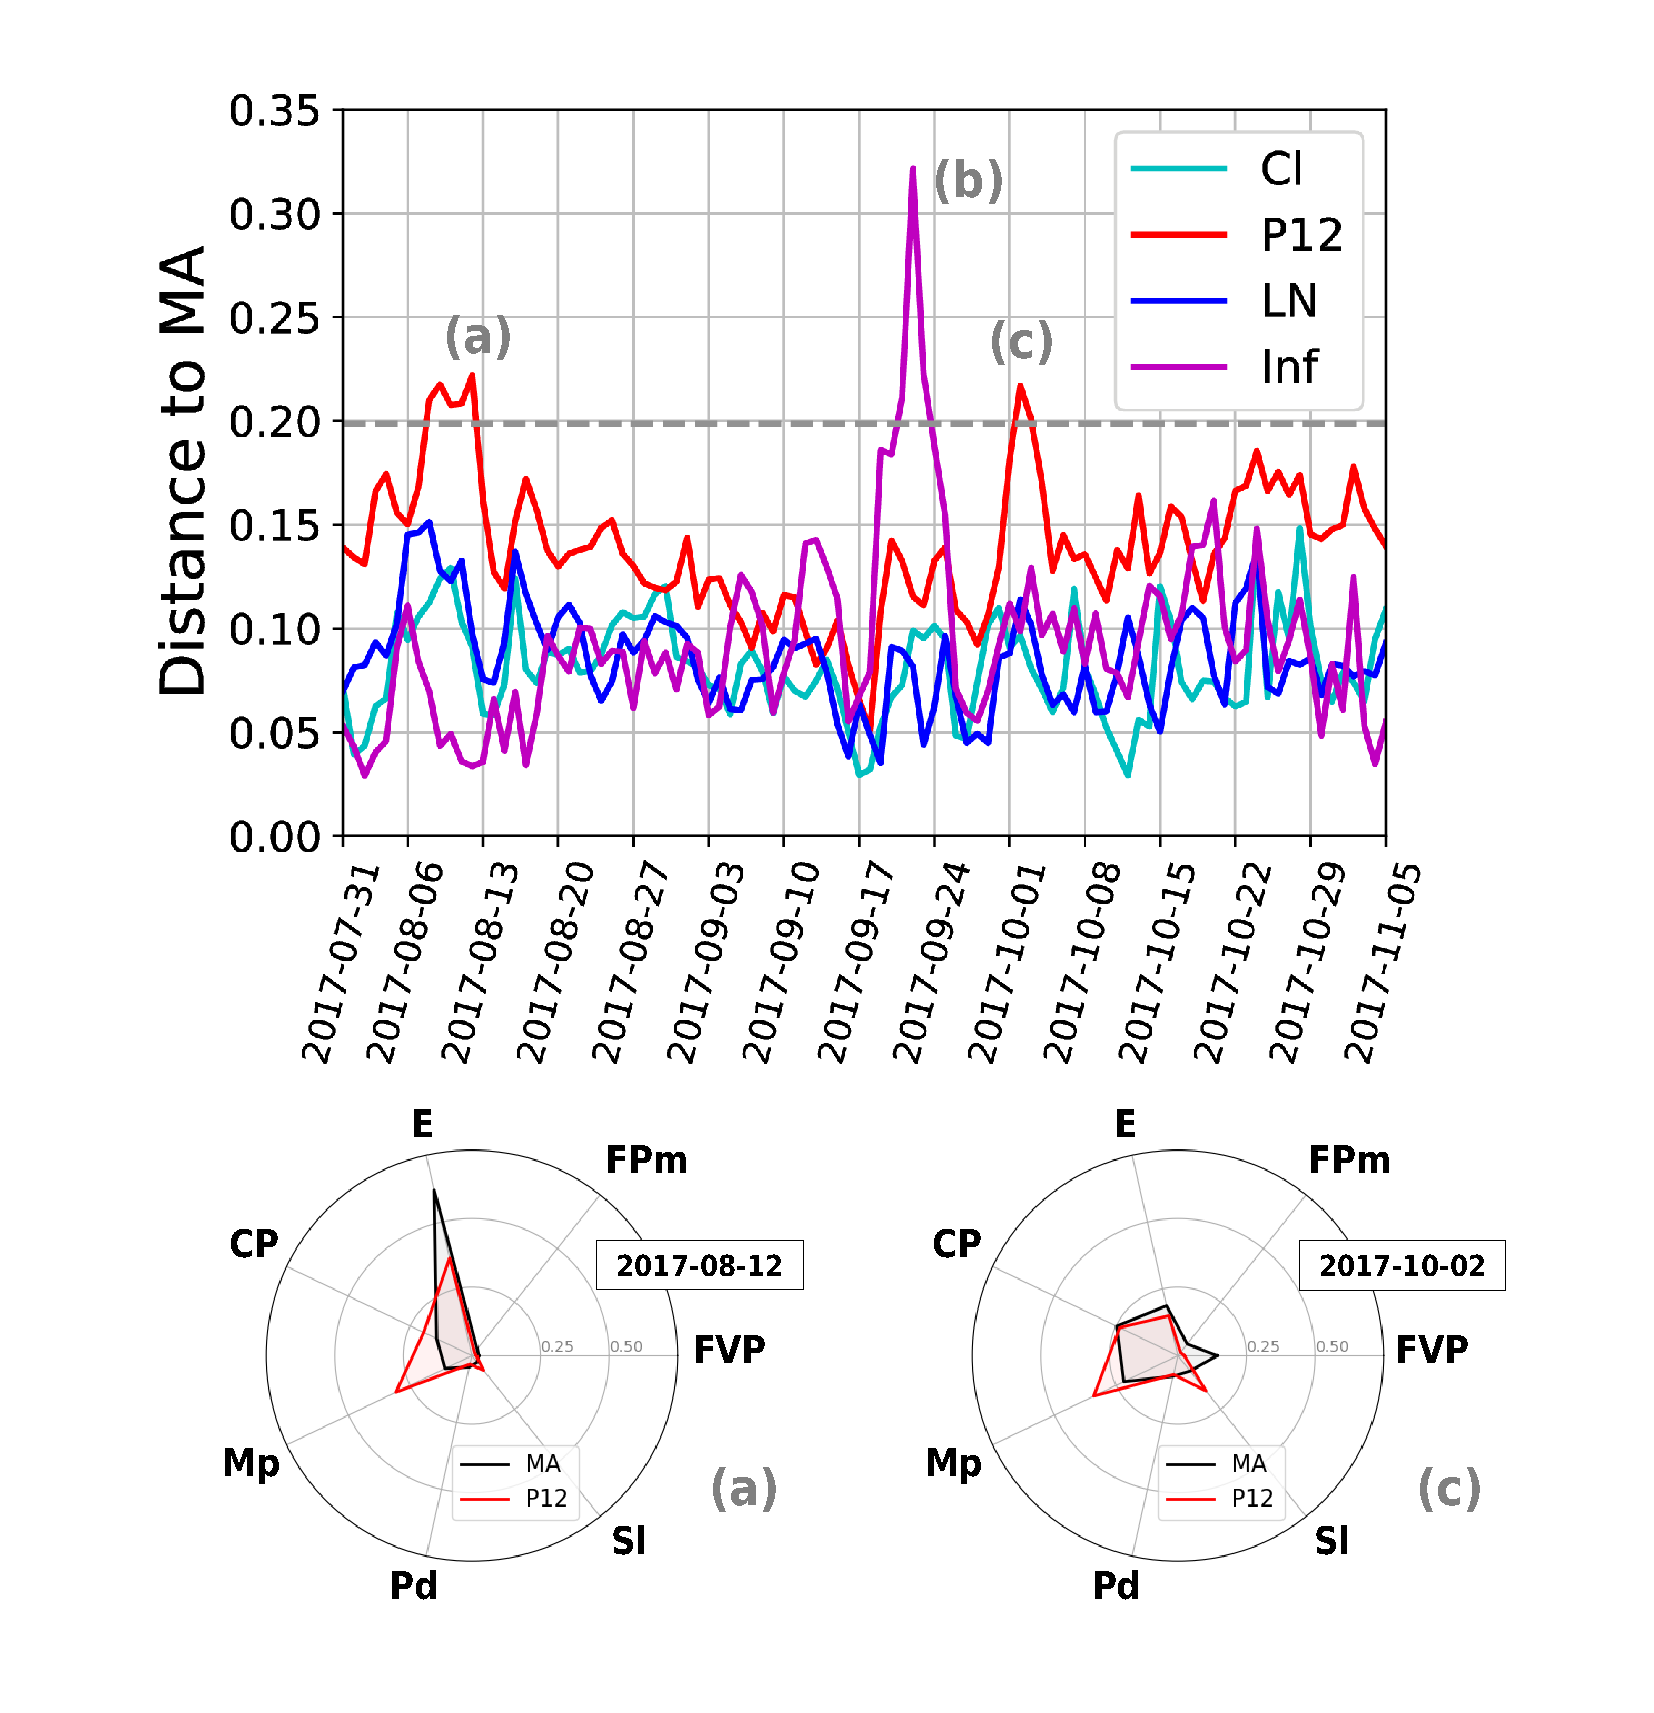
\includegraphics[width = \textwidth]{images/Fig6.pdf}
\caption{\textbf{Jensen Shannon distance between the newspapers’ agenda and the Media Agenda as a function of time.} \emph{Página 12} (P12) shows the more different behavior, motivated again by its interest in the \emph{Missing person} and \emph{Social leader} topics as can be seen in the radar plots which belongs to points (a) and (c). 
The anomalous behavior of \emph{Infobae} (Inf) at point (b) is due to few articles around that date in our database, therefore we ignore its radar plot.}
\label{fig:jensen_shannon_news}
\end{figure}

\subsubsection{Coverage bias}

\par The greater coverage in the topic \emph{Missing person} by \emph{Página 12} is even more clear if we inspect the temporal profile of the topic and compare the coverage given by each newspaper. A difference in the coverage is what it is called \emph{coverage bias}.
In figure \ref{fig:topics_temporal_profiles} we show the temporal profile of the topic \emph{Missing person} (panel (a)) and the topic \emph{Former Planning minister} in panel (b), as an example where the behavior is the opposite, as can be seen below.

\begin{figure}[h]
\centering
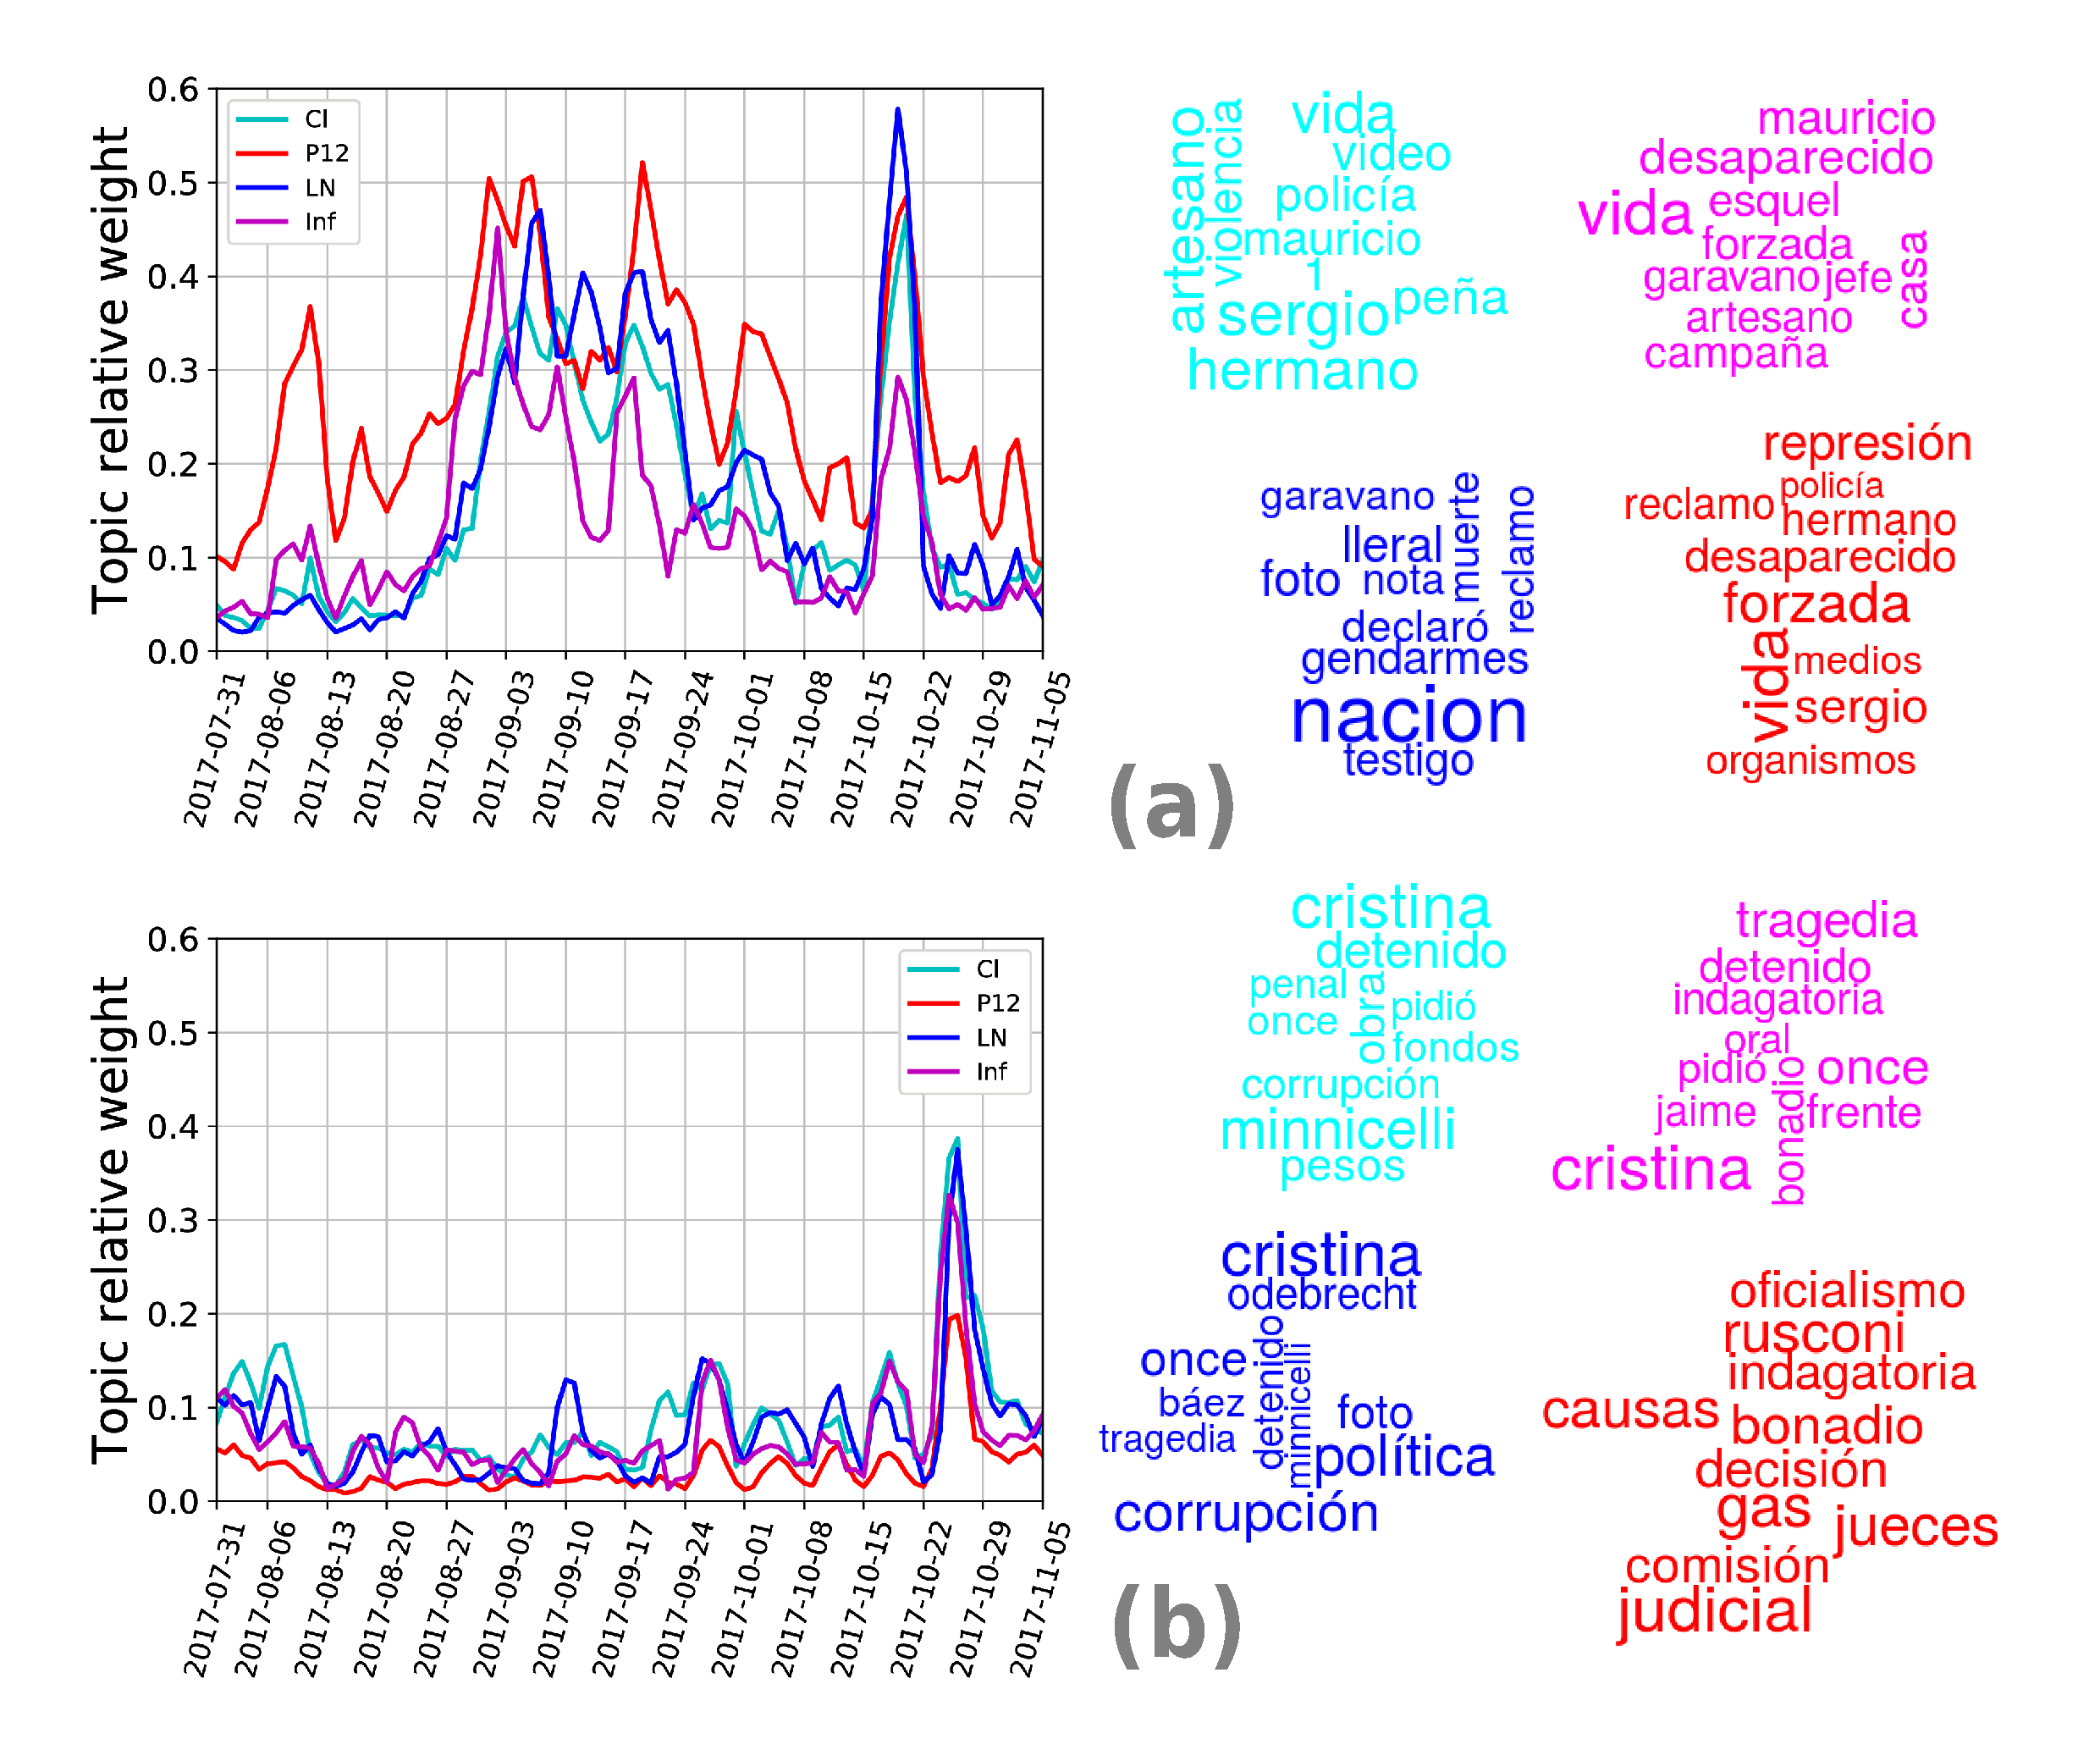
\includegraphics[width = \textwidth]{images/Fig7.pdf}
\caption{\textbf{Relative weight of the topics (a) \emph{Missing person}, and (b) \emph{Former Planning Minister}, and wordclouds of frequent newspapers' keywords}. We interpreted the differences shown in certain periods as an indicator of coverage bias. For instance, in figure (a) Página 12 pays a greater attention in the first days. In the wordclouds, we show which of the defining words are more frequently used by the corresponding newspaper. Most of them are less informative, but other seems to represent a first approximation in the study of framing.}
\label{fig:topics_temporal_profiles}
\end{figure}

\par From panel (a) of figure \ref{fig:topics_temporal_profiles}, we can see a more coverage of \emph{Página 12} respect the other newspapers at the first of the period. We can for instance quantify this difference by the median of the signals. If we focus in the period between July 31th and August 27th, the median of the topic relative weight for \emph{Página 12} is roughly 0.14 and this is statistically significant larger ($p < 10^{-7}$) than other medians, which are lower than 0.05.
Analyzing the same period, but in panel (b), we again can show that the median in \emph{Página 12}, which is roughly 0.01, is lower than the others, which oscillate around 0.05 ($p<10^{-3}$)
This quantification is proposed as method of studying coverage bias in the context of the methodology implemented in our work. 

\par Finally, in figure \ref{fig:topics_temporal_profiles} we also show wordclouds of topic's keywords but separate those that are most frequent mentioned by each newspaper, filtering the words that are common to all and basically define the factual details of the topic.
Although most words are less informative, some are interesting to inspect, for instance, the word \emph{represión} (repression) when \emph{Pagina 12} talks about the topic \emph{Missing Person} and the word \emph{Cristina} (Fernández de Kirchner) which is employed by all newspapers except \emph{Pagina 12} when talk about the topic \emph{Former Planning minister} (see section \ref{sec:Context}).
We don't go farther but we think that a more deeply study of topics' keywords is a first approximation in the study of framing, which will constitute the core of futures works.

\subsection{After all: Who sets the Agenda?}
\label{sec:who_sets}

\par The behaviour of the Media Agenda and the Public one, either by looking at Google Trends or Twitter, shows periods when there is a strong similarity, mostly in the presence of an unexpected event, and periods when seem to be unrelated.
These are mere observation that talk about the correlation between the agendas.
However the agenda-setting theory is in its nature a theory about causations:
Is the audience a passive actor who follows what Media say, or there are periods where the Media must paid attention at public's interests?
Paraphrasing the question, who sets the agenda, the Media or the audience?
In a world where social media exists and the feedback between a Media and its audience is common currency, nowadays the idea that the Media sets the agenda and the audience blindly follows it, as it's seemed to be suggested in the original work of McCombs, is a very weak one. 
\par In spite of the fact that we think that to establish a causation, i.e. the direction towards information flows, is a task that must be made with extreme care, we can not totally skip the question about causation. 
Therefore we will discuss at least in a qualitative way the \emph{Missing person} topic. 
This is the more adequate topic to be discussed because it caused a great impact in either the Media and the audience, and on the other hand, its more important related events are fully contained in the period under studying (see section \ref{sec:Context}).
Therefore we can study the way the topic acquired the importance showed along this work.
\par In figure \ref{fig:Maldonado_setagenda} we show the topic relative weight from the Public Agenda and the Media Agenda. 
After the initial news, the agendas seems to differentiate around August 16th, when the topic started to acquire more importance in the Public Agenda than in the Media, but around August 24th the topic abruptly increase in Public's interest while in the Media the reaction is slower, showing a significant peak in the plot of the discrete differences.
This date is very close to August 26th when a campaign in social media took place. After that, the Media increase its coverage about the topic.
\par Is this a case of reverse agenda-setting, i.e, when the audience set the Media Agenda? 
After all the audience get involved about this topic by the Media, so how was the coverage before those events?
By calculating the cumulative sum we can see how the coverage in a cumulative way was during the first events related to the topic. 
This measure can be seen as the numerical integrate of the temporal profiles of figure \ref{fig:topics_temporal_profiles} between the initial date and the current date. 
It is interesting to note that the newspaper which accumulate coverage during the initial stage was the minority one: \emph{Página 12}. 
Our suggestion of how the agenda was set in this particular topic is the following: one of the newspapers gave great coverage to this one, the audience magnified this in social media and also expressed its interest by reiterative Google searches, and then the rest of the Media oughted to pay attention to this behavior. This suggestion is of course a very reductive one but try to catch in a qualitative way how the information flow was.
On the other hand, behind this interpretation there are two important facts that must be mentioned: First, the disappearance of a person is a very sensible theme for the Argentinian society, and second, there are political reasons in why \emph{Página 12} was particularly interested in cover this topic while the other Media did not follow this interest.

\par We took the question about causation only in a qualitative way. 
There are different metrics that would help in this question, such as Granger causality or correlation by sliding windows. We think that this analysis must be performed with extreme care since the acquirement of the data.
With this work we aimed to provide a quantitative characterization of the behaviour of the Media and the Public but not to establish direction of causation, which we hope this to be the core of future ones.


\begin{figure}
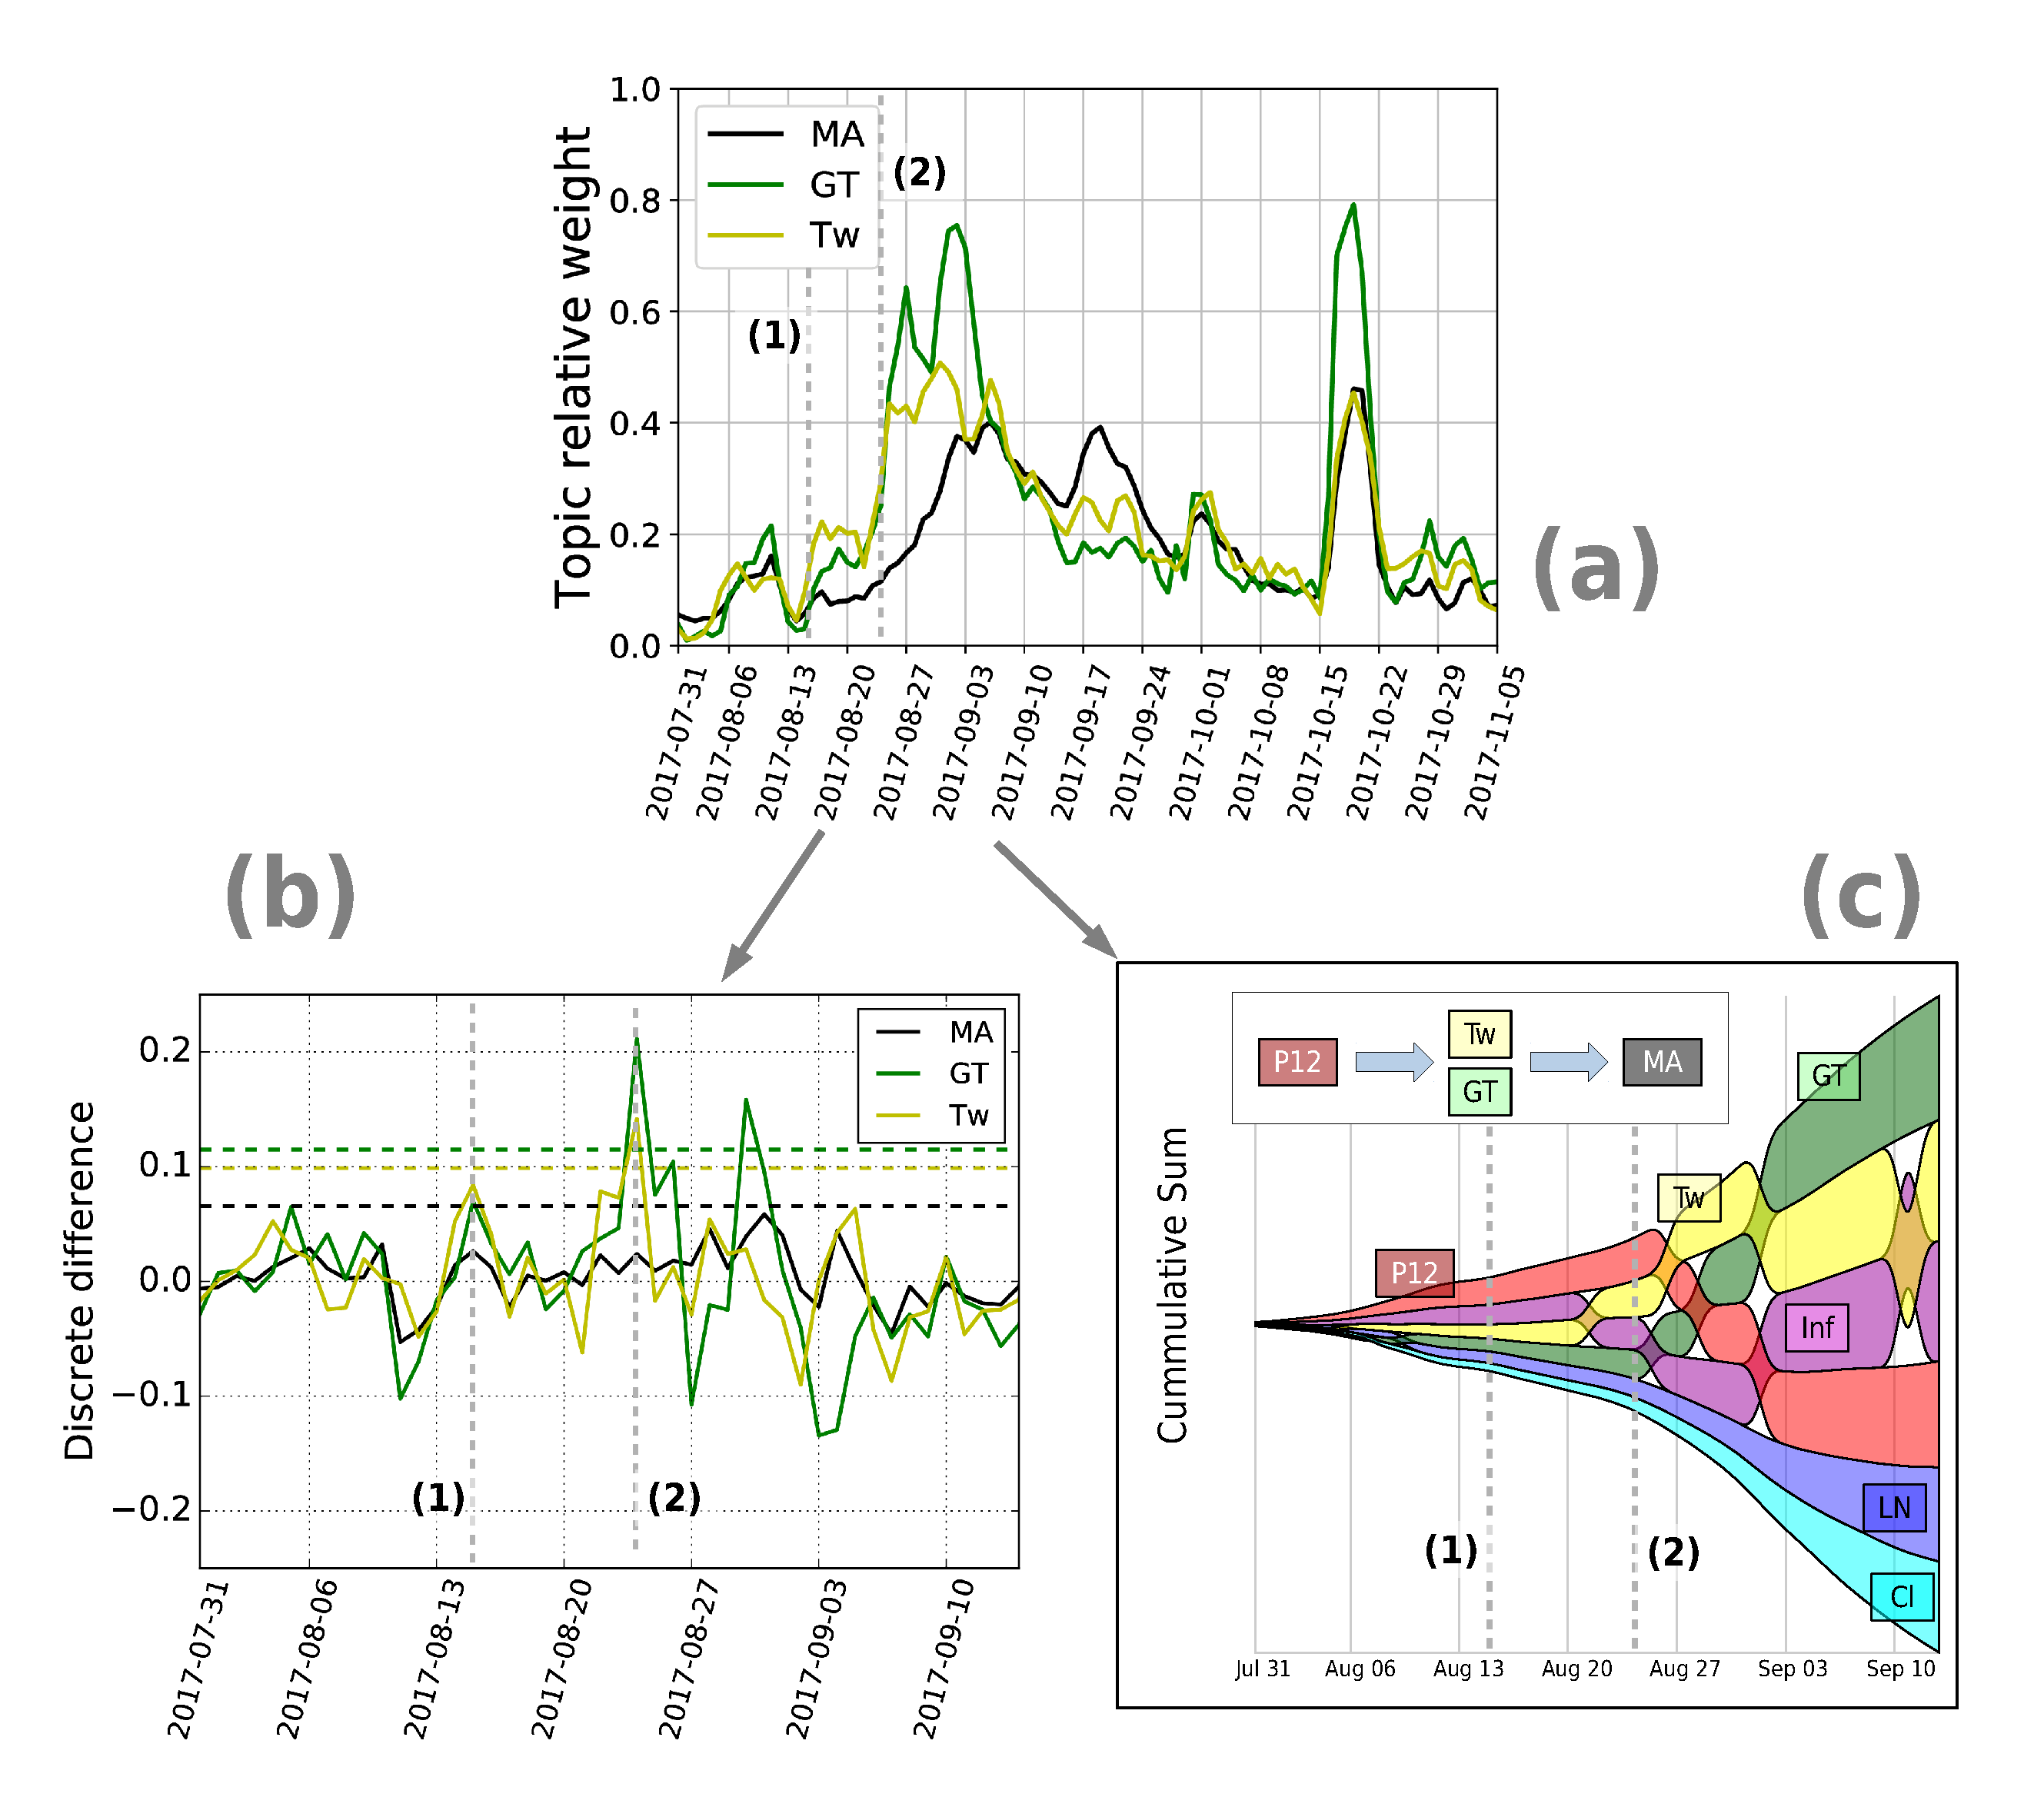
\includegraphics[width = \textwidth]{images/Fig8.pdf}
\caption{\textbf{Agenda setting direction in Missing person's topic?}
The temporal profiles of figure (a) show that the Public increased abruptly its interest in the topic around August 24th, which belongs to the peak \textbf{(*)} shown in figure (b), where the discrete differences were computed. 
This date is also pointed out in the rest of the figures with a vertical grey line together with the asterisk. 
With the computing of the cumulative sum of figure \ref{fig:topics_temporal_profiles} and figure (a), represented as a bump chart in figure (c), we suggest that the topic was first set by \emph{Página 12} and then the Public's interest cause the coverage of the other Media.
}
\label{fig:Maldonado_setagenda}
\end{figure}








\newpage
\section{Supplementary Material}
\subsection{Context}
\label{sec:Context}

\subsubsection{\emph{Elections}}
\par Two legislative elections were celebrated during the period in great part of the Argentina: Primary elections on August 13th and the general elections on October 22th. 
A special focus was put on the elections in the Buenos Aires province, where the former President \emph{Cristina Fernández de Kirchner} participated as a senator candidate representing the alliance \emph{Unidad Ciudadana}, confronting to the alliance \emph{Cambiemos}, which is the alliance of the current President \emph{Mauricio Macri} and the current governor of Buenos Aires province, \emph{Maria Eugenia Vidal}.
 
\subsubsection{Current President}
\par \emph{Mauricio Macri} is the current Argentinian President, since December 2015. 
Most articles in political sections are logically devoted to him under different contexts.
However, it is important to point out that during the period analyzed, and specially after the general elections of October 22th, a controversial labour reform promoted by the government was been discussing.

\subsubsection{\emph{Missing Person}}
\par \emph{Santiago Maldonado} vanished on August 1st after a minor clash between the Gendarmerie (Border Guards) and a group of Mapuches, which recognize as themselves the original population of an area in the Patagonia.
Since that event, the \emph{Mauricio Macri}'s administration was accused by several people as the responsible of a \textbf{forced disappearance}. 
\par A very massive campaign in social media took place on August 26th, under the motto "Where is Santiago Maldonado?", followed by two massive protest marches to the \emph{Plaza de Mayo} took place on September 1st and October 1st, which the first one had a great repercussion due to several incidents that took place during the march.
\par The body of \emph{Santiago Maldonado} was found on 17th October in the \emph{Chubut} river, near the place where he was seen the last time, and the autopsy report told that \emph{Santiago Maldonado} had died from ‘asphyxia after being submerged,’ with no injuries on his body. 
However the responsability of the current administration is still being discussed.

\subsubsection{\emph{Former Planning minister} and \emph{Former Vice-President}}

\par \emph{Julio de Vido} was the Planning minister during the administration of \emph{Nestor Kirchner} and \emph{Cristina Fernandez de Kirchner} (2003-2015). In 2015, he was elected to integrate the Chamber of Deputies, which finally voted to strip \emph{De Vido} of his congressional immunity over corruption allegations and was inmmediatly jailed on October 27th.

\par \emph{Amado Boudou} was the Vice-President of the \emph{Cristina Kirchner}'s administration.
\emph{Boudou} was arrested on November 3th on charges including money-laundering and hiding undeclared assests.

\subsubsection{\emph{Social leader} and \emph{Prosecutor's death}}

\par \emph{Milagro Sala} is an indigenous leader’s. 
She has been incarcerated under pre-trial detention ever since she was first detained in January 2016. She faces allegations of embezzlement related to government funding for housing projects managed by Túpac Amaru, her social organization.
Sala accused the government of "violating her human rights", and several people think that she is a political prisoner of the \emph{Mauricio Macri} administration.

\par \emph{Alberto Nisman} was a special prosecutor who were investigating the 1994 terror attack on the Argentine Israeli Mutual Association (AMIA), until his suspicious death on January 2015.
During the period analyzed in this work, a team of experts led by the Gendarmerie (Border Guard) concluded that late prosecutor's death may have been a case of murder, not suicide.


\subsection{Comparison between NMF and LDA}

\par In this section we apply other topic model, Latent Dirichlet Allocation \cite{blei2003latent} (LDA), to our corpus and compare its results to the shown in this paper. Due to the increasingly use of LDA, we think that a few words about the performance of LDA in our work is necessary. 

\par Naturally the topics found with LDA may not coincide with the NMF ones.
However, one expects that the corpus under studying should be in some manner robust to the election of the topic model.
On the other hand, as was discussed in \cite{o2015analysis}, NMF can be a more suitable topic modeling method in certain domains, in the way that it produces more coherent topics, while LDA tends to return higher levels of generality and redundancy. Topic coherence is defined as the semantic interpretability of the terms used to describe a particular topic, although the coherence of a topic may depend on the end user's expectations.

\par We define a simple coherence measure defined in equation \ref{eq:topic_coherence}, where $d_{ij}$ is the number of documents where the term $i$ and term $j$ appear simultaneously, and $d_{x}$ is the number of documents where appears the term $x$. The summation is over the $N$ top terms of the topic.
It's important to note that if two terms have no co-occurrences, the contribution to the summation is zero, and if these ones appear only together the contribution is one.
A topic with higher coherence is a topic where the terms that define it co-occurrence frequently.

\begin{equation}
TC = \sum_{i < j}^N \frac{2d_{ij}}{d_i + d_j}
\label{eq:topic_coherence} 
\end{equation}

\par We perform a decomposition into 10 topics using LDA with the python module \emph{gensim} \cite{rehurek_lrec}, which allow us to modify the number of times the corpus is read, improving the coherence of the topics.
Unlike to what we see with NMF, the LDA's performance depends strongly on the initial condition of the algorithm. After 10 iterations, we chose the one with highest mean topic coherence, and compared this with the NMF results.

\par In figure \ref{fig:temporal_profiles_nmf_lda} we show the temporal profiles of topics \emph{Elections} and \emph{Missing Person} for both NMF and LDA. The association between topic models was simply made by looking at the topics which share common keywords.
As can be seen from the figure and the table \ref{table:correlation_nmf_lda}, those LDA topics which can be linked to NMF ones or to a combination of these, show a temporal profile highly correlated. 

\par Nevertheless, LDA returns other topics which can not be directly associated, some of them composed of very general words. 
By keeping only those topics which can be associated with NMF and re-defining the Media Agenda over this topic space with reduced dimension, we observed similar results by both methods.  
The same procedure is proposed in absence of an alternative topic model to which make the comparison: Keep only those topics easily interpretable and define the Agendas over this reduced space.
 
\begin{figure}
\centering
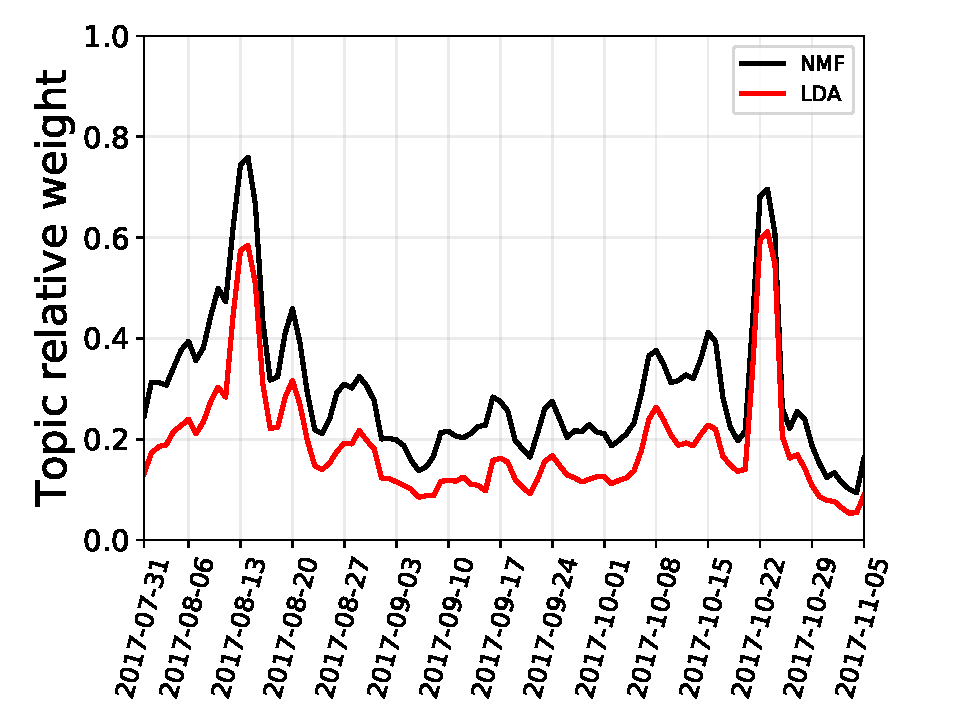
\includegraphics[scale = 0.4]{images/FigA2.pdf}
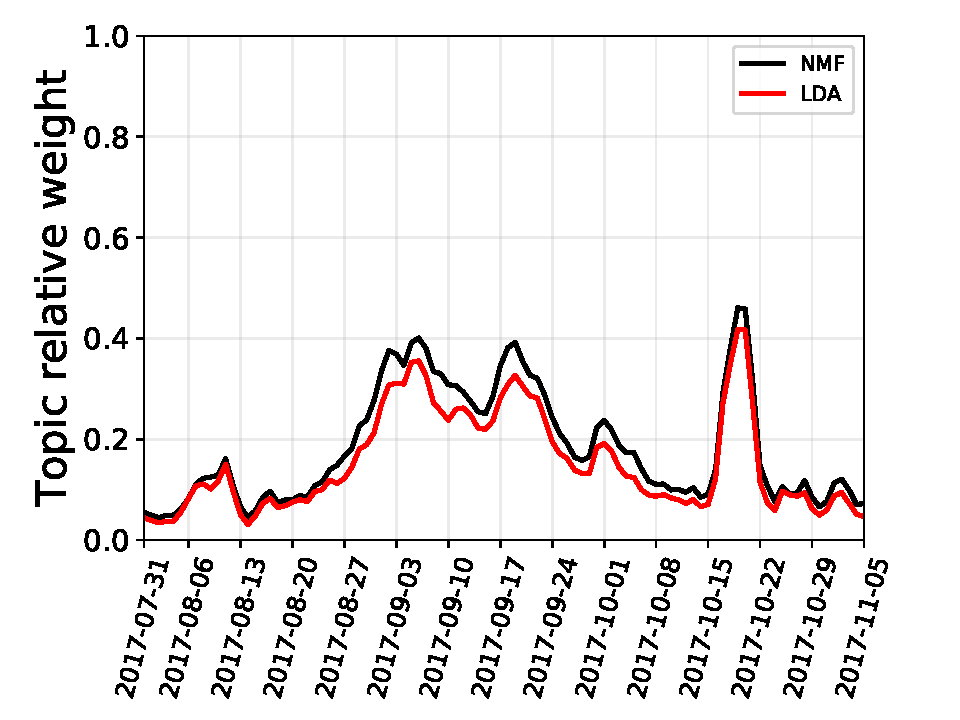
\includegraphics[scale = 0.4]{images/FigA1.pdf}
\caption{Temporal profiles of topics \emph{Elections} (left) and \emph{Missing Person} (right) for both LDA and NMF. All the topics found by applying NMF have a highly correlated counterpart in LDA.} 
\label{fig:temporal_profiles_nmf_lda}
\end{figure}

\begin{table}[h]
\centering
\resizebox{\textwidth}{!}{\begin{tabular}{llc}
\toprule
& Correlation between NMF and LDA \\
\midrule
Elections & \textbf{0.98} \\
Missing person & \textbf{0.99} \\
Former Planning minister + Former Vice-President & \textbf{0.89} \\
Current President & \textbf{0.94} \\
Social leader & \textbf{0.94} \\
Prosecutor's death & \textbf{0.83} \\
\bottomrule
\end{tabular}}
\caption{Correlation between the temporal profiles of the topics found in NMF and associated topics in LDA.}
\label{table:correlation_nmf_lda}
\end{table}

%
\section{Methodology} \label{sec:Methodology}

\subsection{Numerical representation of the corpus}

\par In order to perform the analysis of the articles in the corpus, we describe them as numerical vectors through the \textit{term frequency - inverse document frequency (tf-idf)} representation. \textit{Tf-idf} gives greater values to terms that appear in less documents of the corpus (i.e more specific terms) and/or to those which appear more frequent in a document.

\par Given the set of terms made up by all the corpus' words after removing the non-informative ones, such as prepositions and conjunctions, the \textit{tf-idf} algorithm represents the \textit{i}-document as a vector $v_i = [x_{i1}, x_{i2}, ... , x_{it}]$, where the component $x_{ij}$ is computed by the equation \ref{ec:tfidf}, where $\textrm{tf}_{ij}$ is the number of times the \textit{j}-term appears in the \textit{i}-document, $d$ is the number of documents in the corpus, and $n_j$ is the number of documents where the \textit{j}-term appears. Each document's vector is normalized to unit Euclidean length.
Once the documents' vector are constructed, we join them in a document-term matrix (\emph{M}), which has dimensions of number of documents in the corpus ($d$) per number of terms selected ($t$).

% See parameters of sklearn.feature_extraction.text.TfidfVectorizer
\begin{center}
\begin{equation}
\begin{split}
\text{idf}_{j} & = 1 + \textrm{log}(\frac{1 + d}{1 + n_j}) \\
x_{ij} = \textrm{tf}_{ij} \cdot \textrm{idf}_{j}
\end{split}
\label{ec:tfidf}
\end{equation}
\end{center}

\subsection{Topic detection}
\par We perform \emph{non-negative matrix factorization (NMF)} on the document-term matrix (\emph{M}) in order to detect the main topics in the corpus. 
\emph{NMF} is an algorithm which factorize a matrix \emph{M} into two matrices \emph{W} and \emph{H} (eq.\ref{eq:nmf}), with the property that all three matrices have no negative elements. This non-negativity makes the resulting matrices easier to inspect, and very suitable for topic detection.
\begin{equation}
M^{(d \times t)} \sim H^{(d \times k)} \cdot W^{(k \times t)}
\label{eq:nmf}
\end{equation}
\par As can be seen in eq.\ref{eq:nmf}, the resulting matrix \emph{H} has dimensions of number of documents per $k$, and matrix \emph{W} has dimensions of $k$ per number of terms. The number $k$ is interpreted as the number of topics in the documents and it is a parameter that must be set before the factorization.
The matrix \emph{H} is interpreted as the representation of the documents in the topic-space, and the matrix \emph{W} as the topics represented in the original term-space. 
\par This factorization usually can not be made exactly so it is approximated by minimizing the reconstruction error, i.e. the distance between matrix \emph{M} and its approximated form $\tilde{M} = H \cdot W$. We performed \emph{NMF} through the python module \emph{scikit-learn} \cite{scikit-learn}. % See parameters of sklearn.decomposition.NMF

\subsection{Topic interpretation and temporal profiles}
\par The matrix $H$ obtained by \textit{NMF} gives the representation of the documents in the topic-space. In order to improve its interpretation we normalize each document's vector described in that space to unit $l_1$-norm. Therefore the components of these vectors can be viewed as a degree of membership of a given document in the set of topics. The index of the largest component tells us which is the most representative topic of the document.
\par On the other hand, each row of matrix $W$ represent the topic over the term-space. Therefore, the terms associated with the largest components of the \textit{i}-row are the most representative ones and give an insight of what the topic is talking about.
\par We define the temporal profile of the topic $i$, $W_i(day)$ by the eq. \ref{eq:topic_weight} where $l(j)$ is the number of words of the document $j$, and $h_{ji}$ is the degree of membership of document $j$ on topic $i$. This definition allows all documents to contribute to any topic weight, providing by the fact that each document's vector can have non-zero components in more than one topic.
\par As last steps of the data's preprocessing, we filter the topics' weight in order to reduce the noise but keeping the most details as possible, by redefining $W_i(day)$ as the mean value of a 3 days width window, centered on the day, as described in equation \ref{eq:topic_weight_norm}. 
\par Finally we normalize again all the temporal profiles in order to describe each newspaper as dsitribution over the topics' space which evolves over time. This last normalization prevent us against the differences in the number of articles that each newspaper publishes.

\begin{equation}
W_i(day) = \sum_j^d l(j) \cdot h_{ji} \cdot \delta_{d,day}
\label{eq:topic_weight}
\end{equation}

\begin{equation}
\tilde{W}_i(day) = \frac{1}{3} ({W}_i(day) + {W}_i(day - 1) + W_i(day + 1))
\label{eq:topic_weight_norm}
\end{equation}


\subsection{Outliers identification}
\label{sec:outliers_identification}

\par We identify outliers values in a data set of N observations by following the box plot construction. The quantities (called fences) in \ref{eq:fences} are used, where $Q1$ is the lower quartile (range of the distribution where lies the 25th percent of the data), $Q3$ is the upper quartile (where lies the 75th percent of the data) and $IQ = Q3 - Q1$.

\begin{equation}
\begin{split}
\text{lower inner fence (LIF)} & = Q1 - 1.5  \text{IQ} \\
\text{upper inner fence (UIF)} & = Q3 + 1.5  \text{IQ} \\
\text{lower outer fence (LOF)} & = Q1 - 3  \text{IQ} \\
\text{upper outer fence (UOF)} & = Q3 + 3  \text{IQ}
\end{split}
\label{eq:fences}
\end{equation}

\par A point above the upper inner fence considered a mild outlier and a point aove an outer fence is considered an extreme outlier. The same holds for the lower fences. \footnote{http://www.itl.nist.gov/div898/handbook/prc/section1/prc16.htm}

\subsection{Jensen shannon divergence}

\par In probability theory and statistics, the Jensen–Shannon divergence is a method of measuring the similarity between two probability distributions. It is based on the Kullback–Leibler divergence ($D_{KL}$)\ref{eq:jensen_shannon_distance}, but have useful properties such as it is symmetric and it is always a finite value. The square root of the Jensen–Shannon divergence \ref{eq:jensen_shannon_distance} is a metric often referred to as Jensen-Shannon distance. \cite{fuglede2004jensen}

\begin{equation}
\begin{split}
D_{KL}(P||Q) = -\sum{P(i) log(\frac{Q(i)}{P(i)})} \\
\text{JS Divergence}(P||Q) = \frac{1}{2}[D_{KL}(P||M) + D_{KL}(Q||M)] \\
\text{JS Distance (JSD)} = \sqrt(\text{JS Divergence})
\end{split}
\label{eq:jensen_shannon_distance}
\end{equation}


\subsection{Normalized Shannon's H Information Entropy}

\par The normalized Shannon's entropy \ref{eq:shannon_entropy} as a way to measure how spread is a distribution, taking the maximun value where all outcomes are equally probable in the case of a discrete distribution.

\begin{equation}
H[p] = \frac{- \sum_{i = 1}^{N} p(x_i) * ln(p(x_i))}{ln(N)}
\label{eq:shannon_entropy}
\end{equation}


\newpage
\bibliography{bibliography}

\end{document}
